% Options for packages loaded elsewhere
\PassOptionsToPackage{unicode}{hyperref}
\PassOptionsToPackage{hyphens}{url}
\PassOptionsToPackage{dvipsnames,svgnames,x11names}{xcolor}
%
\documentclass[
  authoryear,
  preprint,
  3p]{elsarticle}

\usepackage{amsmath,amssymb}
\usepackage{lmodern}
\usepackage{iftex}
\ifPDFTeX
  \usepackage[T1]{fontenc}
  \usepackage[utf8]{inputenc}
  \usepackage{textcomp} % provide euro and other symbols
\else % if luatex or xetex
  \usepackage{unicode-math}
  \defaultfontfeatures{Scale=MatchLowercase}
  \defaultfontfeatures[\rmfamily]{Ligatures=TeX,Scale=1}
\fi
% Use upquote if available, for straight quotes in verbatim environments
\IfFileExists{upquote.sty}{\usepackage{upquote}}{}
\IfFileExists{microtype.sty}{% use microtype if available
  \usepackage[]{microtype}
  \UseMicrotypeSet[protrusion]{basicmath} % disable protrusion for tt fonts
}{}
\makeatletter
\@ifundefined{KOMAClassName}{% if non-KOMA class
  \IfFileExists{parskip.sty}{%
    \usepackage{parskip}
  }{% else
    \setlength{\parindent}{0pt}
    \setlength{\parskip}{6pt plus 2pt minus 1pt}}
}{% if KOMA class
  \KOMAoptions{parskip=half}}
\makeatother
\usepackage{xcolor}
\setlength{\emergencystretch}{3em} % prevent overfull lines
\setcounter{secnumdepth}{5}
% Make \paragraph and \subparagraph free-standing
\ifx\paragraph\undefined\else
  \let\oldparagraph\paragraph
  \renewcommand{\paragraph}[1]{\oldparagraph{#1}\mbox{}}
\fi
\ifx\subparagraph\undefined\else
  \let\oldsubparagraph\subparagraph
  \renewcommand{\subparagraph}[1]{\oldsubparagraph{#1}\mbox{}}
\fi


\providecommand{\tightlist}{%
  \setlength{\itemsep}{0pt}\setlength{\parskip}{0pt}}\usepackage{longtable,booktabs,array}
\usepackage{calc} % for calculating minipage widths
% Correct order of tables after \paragraph or \subparagraph
\usepackage{etoolbox}
\makeatletter
\patchcmd\longtable{\par}{\if@noskipsec\mbox{}\fi\par}{}{}
\makeatother
% Allow footnotes in longtable head/foot
\IfFileExists{footnotehyper.sty}{\usepackage{footnotehyper}}{\usepackage{footnote}}
\makesavenoteenv{longtable}
\usepackage{graphicx}
\makeatletter
\def\maxwidth{\ifdim\Gin@nat@width>\linewidth\linewidth\else\Gin@nat@width\fi}
\def\maxheight{\ifdim\Gin@nat@height>\textheight\textheight\else\Gin@nat@height\fi}
\makeatother
% Scale images if necessary, so that they will not overflow the page
% margins by default, and it is still possible to overwrite the defaults
% using explicit options in \includegraphics[width, height, ...]{}
\setkeys{Gin}{width=\maxwidth,height=\maxheight,keepaspectratio}
% Set default figure placement to htbp
\makeatletter
\def\fps@figure{htbp}
\makeatother

\usepackage{booktabs}
\usepackage{longtable}
\usepackage{array}
\usepackage{multirow}
\usepackage{wrapfig}
\usepackage{float}
\usepackage{colortbl}
\usepackage{pdflscape}
\usepackage{tabu}
\usepackage{threeparttable}
\usepackage{threeparttablex}
\usepackage[normalem]{ulem}
\usepackage{makecell}
\usepackage{xcolor}
\usepackage{placeins}
\makeatletter
\makeatother
\makeatletter
\makeatother
\makeatletter
\@ifpackageloaded{caption}{}{\usepackage{caption}}
\AtBeginDocument{%
\ifdefined\contentsname
  \renewcommand*\contentsname{Table of contents}
\else
  \newcommand\contentsname{Table of contents}
\fi
\ifdefined\listfigurename
  \renewcommand*\listfigurename{List of Figures}
\else
  \newcommand\listfigurename{List of Figures}
\fi
\ifdefined\listtablename
  \renewcommand*\listtablename{List of Tables}
\else
  \newcommand\listtablename{List of Tables}
\fi
\ifdefined\figurename
  \renewcommand*\figurename{Figure}
\else
  \newcommand\figurename{Figure}
\fi
\ifdefined\tablename
  \renewcommand*\tablename{Table}
\else
  \newcommand\tablename{Table}
\fi
}
\@ifpackageloaded{float}{}{\usepackage{float}}
\floatstyle{ruled}
\@ifundefined{c@chapter}{\newfloat{codelisting}{h}{lop}}{\newfloat{codelisting}{h}{lop}[chapter]}
\floatname{codelisting}{Listing}
\newcommand*\listoflistings{\listof{codelisting}{List of Listings}}
\makeatother
\makeatletter
\@ifpackageloaded{caption}{}{\usepackage{caption}}
\@ifpackageloaded{subcaption}{}{\usepackage{subcaption}}
\makeatother
\makeatletter
\@ifpackageloaded{tcolorbox}{}{\usepackage[many]{tcolorbox}}
\makeatother
\makeatletter
\@ifundefined{shadecolor}{\definecolor{shadecolor}{rgb}{.97, .97, .97}}
\makeatother
\makeatletter
\makeatother
\journal{Fisheries Research}
\ifLuaTeX
  \usepackage{selnolig}  % disable illegal ligatures
\fi
\usepackage[]{natbib}
\bibliographystyle{elsarticle-harv}
\IfFileExists{bookmark.sty}{\usepackage{bookmark}}{\usepackage{hyperref}}
\IfFileExists{xurl.sty}{\usepackage{xurl}}{} % add URL line breaks if available
\urlstyle{same} % disable monospaced font for URLs
\hypersetup{
  pdftitle={Methods to utilize known habitat to filter data for indices of abundance from a recreational fishery survey in California},
  pdfauthor={Melissa Hedges Monk; Rebecca R. Miller; Cat Memes; Derek Zoolander},
  pdfkeywords={keyword1, keyword2},
  colorlinks=true,
  linkcolor={blue},
  filecolor={Maroon},
  citecolor={Blue},
  urlcolor={Blue},
  pdfcreator={LaTeX via pandoc}}

\setlength{\parindent}{6pt}
\begin{document}

\begin{frontmatter}
\title{Methods to utilize known habitat to filter data for indices of
abundance from a recreational fishery survey in California}
\author[1]{Melissa Hedges Monk%
\corref{cor1}%
\fnref{fn1}}
 \ead{melissa.monk@noaa.gov} 
\author[2]{Rebecca R. Miller%
%
\fnref{fn2}}
 \ead{bob@example.com} 
\author[2]{Cat Memes%
%
\fnref{fn3}}
 \ead{cat@example.com} 
\author[]{Derek Zoolander%
%
}
 \ead{derek@example.com} 

\affiliation[1]{organization={Southwest Fisheries Science
Center}, addressline={110 McAllister Way}, city={Santa
Cruz}, country={}, postcode={95060}}

\affiliation[2]{organization={Another University}, addressline={Street
Address}, city={City}, country={}, postcode={Postal Code}}


\cortext[cor1]{Corresponding author}
\fntext[fn1]{This is the first author footnote.}
\fntext[fn2]{Another author footnote, this is a very long footnote and
it should be a really long footnote. But this footnote is not yet
sufficiently long enough to make two lines of footnote text.}
\fntext[fn3]{Yet another author footnote.}

        
\begin{abstract}
This is the abstract.
\end{abstract}





\begin{keyword}
    keyword1 \sep 
    keyword2
\end{keyword}
\end{frontmatter}\ifdefined\Shaded\renewenvironment{Shaded}{\begin{tcolorbox}[interior hidden, boxrule=0pt, frame hidden, sharp corners, enhanced, borderline west={3pt}{0pt}{shadecolor}, breakable]}{\end{tcolorbox}}\fi

\hypertarget{introduction}{%
\section{Introduction}\label{introduction}}

Melissa will refocus the introduction - I keep changing my mind.

Integrated fisheries stock assessment models utilize a variety of data
sources to develop the most complete picture of the stock and current
status in relation to management thresholds.

Catch per unit effort is one

More often(TYPICALLY??), an index of abundance is used as a relative
measure of the population and requires a time series to inform the stock
assessment model. An index of relative abundance assumes that changes in
the index are proportional to changes of abundance in the population
\citep{Harley:2001:CUE}. Fishery-independent data collected from
standardized survey designs provide a more unbiased estimation of the
trend in a fisheries population. However, fishery-independent surveys
are costly, labor intensive and often require a long time series to be
considered informative in fisheries stock assessments. In an ideal
situation, both fishery-dependent and fishery-independent surveys would
be used to inform the stock assessment model. However, there are cases
when only fishery-dependent data are available and the caveats of each
data stream must be considered (cite assessments). Fishery-dependent
data are collected directly from the the fishery and are less costly
than (than what????) the whose operations are not constrained by
sampling designs, but dependent on the behaviors of the captain and
vessel and, in the case of recreational trips, customer preference.

Fishery-dependent surveys sample the fishing fleets and are subject to
potential sampling biases. The sampling is dependent on the fishing
boat's behavior, which is to maximize catch. Sampling of the fishing
fleet is often opportunistic based on the availability of samplers and
the availability of trips to sample. Sampling the fisheries can also be
constrained to the current regulations, which may prohibit the retention
of a species or fishing at certain depths, i.e., California Department
of Fish and Wildlife has varying spatial and temporal depth and season
closures implemented through six management regions. There is also a
network of Marine Protected Areas (MPAs) designated from 2007-2012 that
prohibit recreational fishing, and are therefore areas no longer sampled
by the recreational fishing fleet.

\emph{Catch per unit effort (CPUE) is a common metric available from
fishery-dependent surveys \citep{Maunder:2004:SCE}.}

A common characteristic of ecological data is a high proportion of zero
observations across samples and the question as to whether the sampling
occurred within the species' habitat and the species was not observed or
if the sampling occurred outside of the species' habitat (structural
zeroes). \textbf{you might mention someplace in introduction that
nearshore rockfish are strongly associated with rocky habitat-- perhaps
here. Also, consider this sentence/paragraph as the opening paragraph??}
Fisheries survey data are often subset to exclude structural zeroes
using the Stephens-MacCall method \citeyearpar{Stephens:2004:MAS}, which
models the probability of observing the target species given the other
the presence/absence of other species. However, the onboard observer
survey collected location-specific information on each observer fish
encounter. To subset the onboard observer survey data and exclude
structural zeroes,we used the positive catch locations (I DON''T TOTALLY
UNDERSTAND THIS SENTENCE- only postiive catches are included?) this
sentence seems like it is in the wrong place? more of a methods?) as a
proxy for suitable habitat.

The Pacific Fishery Management Council's Groundfish Fishery Management
Plan (FMP) contains 64 groundfish species off the West Coast of the
United States. The data needs are large and as of 2022, xx xx species
have not had a full age-structured stock assessment in at least one area
of the coast, e.g., yellowtail rockfish (\emph{Sebastes flavidus})and
kelp greenling (\emph{Hexagrammos decagrammus}) do not have accepted
stock assessments for California. In some cases a stock assessment may
be categorized as data rich, but the only index of abundance available
is from a fishery-dependent CPUE time series of observed recreational
angler catch rates \citep{Cope:2013:ISC}. (THIS PARAGRAPH SEEMS LIKE IT
MIGHT BETTER FIT HERE?? or state in a sentence that this work will help
future stock assessments as a lead in to the next paragraph?? How do
groundfish stock assessments typcially filter data? \textbf{Is that the
stevensMacall method??} As a lead in to the next paragraph??)

To explore the changes \textbf{(of what? index of abundance results??
the number of records included?)} in data filtering related to
structural zeroes, we utilized high resolution fishery sampling and
bathymetry data. We evaluated data from a recreational party boat
onboard observer program, which collects location- and species-specific
CPUE information from the commercial passenger fishing vessel (CPFV;
also know as party boat) fleet \citep{Monk:2014:DRD}. The data were
collected at the level of a fishing drift and fine-scale habitat data
are available for a large fraction of California state waters. Paired
with recently available high-resolution bathymetry data provided an
opportunity to overlay each individual fishing drift onto known habitat
type (hard vs.~soft substrate), and has been the method utilized for
stock assessments since 2015. To explore how data selection methods and
the resulting indices would change if the data were only available at a
courser resolution, we used the same data set to develop standardized
indices of relative abundance based on three different data filtering
methods. We applied these methods across six nearshore rockfish species
with different life histories,habitat preferences and commonness in the
data.

The three data treatment methods included filtering the drift-level data
based on known location, i.e., the status quo \textbf{(what is status
quo? StevensMcCall?}), treating the drift-level data as if the location
of the drifts were not available, and lastly, an aggregating of the
catches at the drift-level data to a trip. In addition, for the model
filtered based on known rocky reef habitat, we weighted the index by
area of habitat within pre-defined regions. For the two cases where we
removed the location information, we filtered the data using the
Stephens-MacCall method.

The Stephens-MacCall \citeyearpar{Stephens:2004:MAS} filtering approach
was used to predict the probability of encountering the target species,
based on the species composition of the catch in a given trip. The
method uses presence/absence data within a logistic regression to
identify the probability of encountering a target species given the
presence or absence of other predictor species. This method is commonly
used to filter data that were collected dockside after a vessel returned
to port or when location data are not provided.

Prior to 2013, these data had not been used to develop an index of
abundance for West Coast fisheries stock assessments. That was partially
due to the availability of data and at that point in time not many full
stock assessments had been conducted for the nearshore groundfish
species. These data were first used without the habitat data in a suite
of 2013 data moderate stock assessments \citep{Cope:2015:DMS}, where
data were filtered using positive species observations and an alpha hull
method commonly used to estimate species home range sizes and
distribution modeles for terrestrial species
\citep{Burgman:2003:BSR, Meyer:2017:CHM}

\emph{cut from another place: The onboard observer data provide a
high-resolution of catch, effort and the ability to map the fishing
drifts to fine-scale habitat data. This paper explores methodological
differences in data treatment to see what we gain by having the
high-resolution habitat data and using that as a mechanism to filter out
trips that are not targeting the species of interest}

\emph{This paper explores methodological differences in data treatment
to determine changes in trends in indices and the associated error among
three alternative assumptions and data filtering strategies. All of the
methods described below started with the same subset of drifts from the
onboard observer data, restricted to state waters and the years
2004-2016. In the case of application to stock assessments, all
potential data are explored, which may be why trends in indices differ
in this paper than what has previously been published in stock
assessments. Since the most recent stock assessments in 2021, the data
have undergone a major quality assurance effort by the authors.}

\hypertarget{methods}{%
\section{Methods}\label{methods}}

**Grammatical tense is not my forte for methods so please advise**

We applied the methods described in the following sections to develope
indicies of abundance for six species (or species pairs) of rockfish
(\emph{Sebastes spp.}) that are of management interest on the West
Coast: black rockfish (\emph{Sebastes melanops}), the blue and deacon
rockfish (\emph{Sebastes mystinus}, \emph{Sebastes diaconus}), brown
rockfish (\emph{Sebastes auriculatus}), China rockfish (\emph{Sebastes
nebulosus}), gopher rockfish (\emph{Sebastes carnatus}), and the
vermilion and sunset rockfish (\emph{Sebastes miniatus}/\emph{Sebastes
crocotulus}). All of these species are managed within the of the complex
of West Coast rockfishes that inhabit the nearshore waters {[}cite
FMP{]}. The two cryptic species pairs (blue/deacon and sunset/vermilion
rockfish) are genetically identifiable, but not separable within the
onboard observer data time series and both cryptic pairs are currently
managed as species complexes by the Pacific Fisheries Management Council
\citep{Bizzarro:2020:GIB, Longo:2022:GMR}. These six species all have
different latitudinal distributions, exploitation histories, habitat and
depth preferences, and live history strategies\citep{Love:2002:RNP}. We
will discuss the importance of consideration for these differences in
development of indices of abundance.

\hypertarget{survey-data-and-habitat-base-filtering}{%
\subsection{Survey Data and Habitat-base
Filtering}\label{survey-data-and-habitat-base-filtering}}

The California Department of Fish and Wildlife (CDFW) began a
fishery-dependent onboard observer survey of the Commercial Passenger
Fishing Vessel (CPFV or party/charter boat) fleet in 1999. In 2004, the
survey became part of the CDFW's California Recreational Fisheries
Survey (CFRS) that includes additional surveys to quantify catch and
effort by the recreational fleet. In response to a request from the
fishing industry, the California Polytechnic State University Institute
of Marine Science, San Luis Obispo (Cal Poly) began a supplemental
onboard observer program in 2001 of the CPFV fleet based in Port Avila
and Port San Luis along the Central Coast {[}\#fig-map{]}. Both the CDFW
and the Cal Poly onboard observer surveys continue through present day;
however, due to both spatial and temporal recreational regulation
changes we limited the dataset for this research to the years 2004 to
2016. Between 1999 and 2003, the recreational regulations evolved from
no restriction on the number of lines or hooks an angler could deploy to
a one line and two-hook maximum, as well as implementation of depth
restrictions. These were a direct result of ten groundfish species
declared overfished in 2000 the entire West Coast groundfish fishery was
declared a federal disaster \citep{Conway:2008:SLL}. Subsequent
management and successful rebuilding of all but one groundfish stock
(yelloweye rockfish, \emph{Sebastes ruberrimus}) allowed a relaxation of
depth restrictions beginning in 2017 and shifted fishing effort
\citep{Monk:2021:SVR}.

While only a small portion of the total CPFV trips taken are observed,
the onboard observer program collects a large amount of data during each
trip. During each trip the sampler records information for each fishing
drift, defined as a period starting when the captain announced ``lines
down'' to when the captain instructs anglers to reel their lines up.
Just prior to the start of each fishing drift, the sampler selected a
subset of anglers to observe, at a maximum of 15 anglers per drift. The
sampler records all fish encountered (retained and discarded) by the
subset of anglers as a group, i.e., catch cannot be attributed to an
individual angler. Samplers also record the start and end times of a
drift, coordinates of the fishing drift (start latitude/longitude and
for most drifts, end latitude/longitude), and minimum and maximum bottom
depth. Fish encountered by the group of observed anglers are recorded to
the species level as either retained or discarded. This provides
information on the catch (count of each species) and effort (time and
number of anglers fished) during each fishing drift. While both surveys
include records of discarded fish, we only used the retained catch in
these analyses. Discarded fish can often represent a different size
structure than retained fish, either due to size limits or angler
preference, or represent fish encountered during a temporal or spatial
closure.

The SWFSC developed a relational database for the CDFW onboard survey
from 1999-2010 and additional survey details can be
found\citeyearpar{Monk:2014:DRD}, and we received more current data from
the CDFW. The Cal Poly data are provided to the SWFSC annually. All data
were cross-checked for potential errors at the drift-level by SWFSC
staff; where identifiable errors could be corrected within the CDFW
database (e.g., obvious transcription of latitude or longitude), we made
those changes and noted them in the database. Potential errors
identified in the Cal Poly database were checked against the original
datasheets and corrected when appropriate.

The combined data north of Point Conception from 2004-2016 contained a
total of 19,425 fishing drifts and after removing drifts with missing
effort information (time fished or observed anglers), 19,180 drifts
remained. To further remove drifts that may not accurately define a
successful fishing drift or represent data errors, the upper and lower
1\% of the recorded time fished and recorded observed anglers were
removed. This resulted in fishing drifts lasting between three and 96
minutes and three to 15 observed anglers, reducing the data to 18,591
fishing drifts. Given that the fishery was closed deeper than 40 fathoms
for the entire time period from 2004-2016, we filtered the data to
retain 99\% of all drifts (18,405 drifts) based on average drift depth,
a cutoff of 46.6 fathoms. We calculated average depth from the recorded
minimum and maximum depths when available or the imputed minimum and
maximum depth from the bathymetry layer described in the next paragraph.
A depth cutoff slightly deeper than the maximum allowed is reasonable
given the rugous habitat fished and all retained drifts occurred within
California state waters.

Recently collected high resolution seafloor mapping data allowed us to
overlay each drift from the onboard observer programs with predicted
habitat. We utilized the bathymetry and backscatter data collected by
the California Seafloor Mapping Program (CSMP) {[}@Golden:2013:CSW{]}.
The CSMP formed in response to the network of Marine Protected Area
network established in California state waters. The CSMP mapped
California state waters (3 nm from shore) at a 2 m resolution north of
of Point Conception (\(34^\circ 27^\prime N\)) to the California-Oregon
border. Rough and smooth substrates were identified by CSMP using two
rugosity indices, surface:planar area, and vector ruggedness measure
(VRM) of the bathymetric digital elevation model. The CSMP set a varying
VRM threshold for each block, removed any artifacts, and is considered a
conservative estimate of rough habitat. A total of 133 CSMP substrate
blocks were mosaiced together by authors. Authors then converted the
rough habitat (rocky habitat proxy) from a raster format to polygon, and
performed 5 m buffer to the rough habitat polygon to allow for any
potential inadvertant error in positional accuracy. Reef polygons
greater than or equal to 100 \$m\^{}2\$ were included. Contiguous
polygons identified as rocky substrate remained as a singular rocky
reef, regardless of size. Reefs were grouped where any reef polygon
greater than a distance of 200 m was considered a separate rocky reef.
The 200 m distance criteria was based on a spatial scale meaningful for
nearshore rockfish that exhibit site high fidelity, where tagging
studies have recaptured rockfish close to original capture sites
\citep{Lea:1999:BAM, Matthews:1985:SSM, Hannah:2011:SFM, Hannah:2012:UNC}.
The area of rocky habitat for this paper was calculated to exclude
portions of the reef that extended outside of California state waters
(further than 3 nm from shore). The mapped area does not include the
white zones close to shore, which extends approximately 200-500 m from
the shoreline. Fishing by the CPFV fleet is limited in the white zone
due to shallow depths and kelp beds. We assigned fishing drifts to reefs
based on the recorded start location of a drift, given that the end
locations of drifts were not always recorded, and in the interest of
maximizing effort, we did not quality check the end locations. The
distance from the recorded drift start location to the nearest rocky
habitat was calculated in meters. For each target species, we calculated
the cumulative distribution of distance to rocky reef for drifts that
retained the target species and used a distance cutoff of 90\% for each
species. The distance cutoff for blue, China and gopher rockfish was six
meters, eight meters for vermilion rockfish, 14 meters for black
rockfish and 16 meters for brown rockfish.

\hypertarget{stephens-maccall-data-filtering}{%
\subsection{Stephens-MacCall Data
Filtering}\label{stephens-maccall-data-filtering}}

It is not often the case where high-resolution habitat and fishing
location information are both available, and for many fishery-dependent
surveys an analyst will have to determine which subset of the data to
use based on available information. The onboard observer data provide an
opportunity to explore what information we gain from explicit knowledge
of fishing locations. We took the same data and removed any location
identifiers and also aggretated data across a fishing trip to see how
each affects data selection and the resulting indices of abundance.

We applied the Stephens-MacCall method to both the drift-level data and
the trip-level data \citeyearpar{Stephens:2004:MAS}. Prior to any
filtering a total of 19,425 drifts that aggregated to 2,270 trips were
available for the analyses. The number of initial samples used for the
Stephens-MacCall filtering method were higher than the habitat-informed
data described in the previous section because we retained drifts with
missing effort or location data, which allowed us to retain as much
information about a trip as possible.

Before applying the Stephens-MacCall method, we identified a suite of
potentially informative predictor species for each of the six target
species. Species that never co-occurred with the target species and
those present in fewer than 1\% of all drifts and 3\% of all trips were
removed to reduce the number of species to those that were informative.
A lower threshold was selected for the drift-level data to the change in
magnitude of the number of samples when using drifts vs trips.

The remaining species all co-occurred with the target species in at
least one trip and were retained for the Stephens-MacCall logistic
regression. Coefficients from the Stephens-MacCall analysis (a binomial
generalized linear model) were positive for species that are more likely
to co-occur with the target species, and negative for species that were
less likely to be caught with target species. The intercept represented
the probability of observing only the target species in a sample. We
also calculated the 95\% confidence interval for each coefficient.

Stephens and MacCall \citeyearpar{Stephens:2004:MAS} recommended
including all trips above a threshold where the false negatives and
false positives are equally balanced. However, this theshold does not
have any biological relevance and for this particular data set where
trained samplers identify all fish. We assumed that if the target
species was encountered, the vessel fished in appropriate habitat.
Stephens and MacCall \citeyearpar{Stephens:2004:MAS} proposed filtering
(excluding) samples from index standardization based on a criterion of
balancing the number of false positives and false negatives from the
predicted probability of encounter. False positives (FP) are trips that
are predicted to encounter the target species based on the species
composition of the catch, but did not. False negatives (FN) are trips
that were not predicted to encounter the target species, given the catch
composition, but caught at least one target species.

Of interest for the index of abundance was the elimination of trips that
had a low probability of catching the target species given the other
species caught on the trip. Therefore, we retained all of the trips that
caught the target species and those trips that did not catch the target
species, but had a probability higher than the threshold balancing the
false negatives and false positives. This practice has commonly been
used in recent stock assessments of rockfish on the West Coast.

\hypertarget{indices-of-abundance}{%
\paragraph{Indices of Abundance}\label{indices-of-abundance}}

Four standardized indices of abundance were generated for each of the
six species, one each for the data filtering method (drift-level habitat
informed, Stephens-MacCall filtered drift-level, Stephens-MacCall
filtered trip-level) and an area-weighted index from the
habitat-informed drift-level data. All indices were modeled using
Bayesian generalized linear models (GLMs) and the delta method
\citep{Lo:1992:IRA}. The delta GLM method is commonly used to
standardize catch-per-unit effort for stock assessments {[}citations{]}.
The delta method models the the data with two separate GLMs; one for the
probability of encountering the species of interest from a binomial
likelihood and a logit link function and the second models the positive
encounters with either gamma or lognormal error structure. The error
structure of the positive model was selected via AIC from models with
the full suite of considered explanatory variables.

The response variable for the positive models was angler-retained catch
per unit effort. For the indices modeled at the level of a drift, effort
was calculated as the number of angler hours fished on a drift. The
trip-level effort was calculated as angler days, using the average
number of observed anglers across all drifts on a trip.

To keep comparisons across data filtering methods similar, depth was not
considered as an explanatory variable in the habitat-informed index.
Depth is often a significant explanatory variable for rockfish species,
with many rockfish species and populations separated by depth
\citep{Love:2002:RNP}. Year was always included in as an explanatory
variable in model selection, even if it was not significant, because the
goal of the index of abundance was to extract the year effect. Other
explanatory variables considered for the habitat-informed index were the
rocky reefs and wave (a 3-month aggregated period of time, e.g.,
January-March). The area-weighted index also included a year/rocky reef
interaction term, even if it was not statistically significant, to allow
us to weight the index by the area of rocky reef. The areas of rocky
reef were aggregated differently for each species to ensure adequate
sample sizes to explore the year/rocky reef interaction.

Explanatory variables for the two indices that were blind to habitat
information included only year, wave and region, i.e., aggregated
counties of landing. California has 14 coastal counties north of Point
Conception, 11 of which were represented in these data. We aggregated
the northern counties of Del Norte, Humboldt and Mendocino into one
region, Sonoma and Marin counties just north of San Francisco into
another region and Alameda and San Francisco counties into a third
region. The remaining counties of San Mateo, Santa Cruz, Monterey and
San Luis Obispo remained unaggregated.

The the model of positive samples, the gamma or lognormal error
distribution was chosen via maximum likelihood AIC from the full model
with all explanatory variables. Model selection for the binomial and
positive observation models were also selected using AIC and unless very
different predictors were selected, the same predictors were used in
each of the two Bayesian models. The Bayesian models were run with 5,000
iterations and uninformative priors. Posterior predictive model checks
were examined for both the binomial and positive observation models,
including the predicted percent positive compared to the maximum
likelihood estimates. We constructed the final year index by multiplying
the back-transformed posterior draws from the binomial model with the
exponentiation of positive model draws, and taking the mean and standard
deviation for each year.

The area-weighted index was developed by extracting the posterior draws
of from each year and area combination of the binomial and positive
posterior predictions, and then summing across the product of the
posteriors weighted by the fraction of total area within each reef. To
compare the indices across the three data filtering methods and the
area-weighted index, each index was scaled to its mean value.

Versions of the indices filtered based on habitat were approved by the
Pacific Fisheries Management Council's Science and Statistical Committee
for use in the 2013 stock assessments and have been used all of the
stock assessment process since. Comparisons should not be drawn between
the indices presented here and the stock assessment documents as the
indices in this paper were simplified to develop direct comparisons
among methods.

\hypertarget{results}{%
\section{Results}\label{results}}

\hypertarget{survey-data-and-habitat-assignment}{%
\subsection{Survey Data and Habitat
Assignment}\label{survey-data-and-habitat-assignment}}

The data sets were filtered for errors within the relational database
before analyses and the data used here reflects changes from the QA/QC
process that may not be reflected in data available directly form CDFW.
The addition of the Cal Poly survey to the CDFW survey increased the
sample sizes of observed trips out of San Luis Obispo county by an
average of 155\% from 2004-2016.

Approximately 21\% of the CDFW observed groundfish trips were north of
Point Conception, which is xxx to the xxx\% of estimated charter boat
effort across the state {[}pull and cite RecFIN{]}. North of Bodega Bay,
California the majority of charter boats are smaller 6-pack vessel that
may not have the capacity to carry an observer onboard.

We defined 108 areas of rocky habitat on the finest scale within
California state waters from Point Conception to the California/Oregon
border. After exploratory analyses and considering the the availability
of data, the areas rocky habitat was grouped into six regions to ensure
adequate sample sizes for developing indices of abundance (Figure
@fig-map). While covering a small area, the number of available samples
from the Farallon Islands off the coast of San Francisco was high enough
to warrant keeping it as a separate area of rocky habitat. The region
defined from the California/Oregon to San Francisco encompasses 49\% of
the total rocky habitat in state waters by area, but only 12\% of the
observed drifts fished in this area, and represents approximately 9\% of
the total effort. Each of the four remaining nearshore regions from San
Francisco to Point Conception contained an average of 11\% of the
available habitat.

Bay: 38\% effort

Central: 53\%

Redwood: 4\%

Wine: 5\%

The CDFW manages recreational fisheries by counties aggregated to
districts, four of which are north of Point Conception. The

The distribution of the speci

, i.e., black rockfish has a more northerly distribution reflected in
the aggregation of data from Santa Cruz and south, whereas brown
rockfish is distributed across coastal California (Figure xxx).

While the filter is useful in identifying co-occurring or non-occurring
species assuming all effort was exerted in pursuit of a single target,
the targeting of more than one species or species complex (``mixed
trips'') can result in co-occurrence of species in the catch that do not
truly co-occur in terms of habitat associations informative for an index
of abundance.

A look at the distirbution of each species by the percent of positive
observations (over all years) and the average CPUE at the drift-level by
aggregated areas of rocky habitat are presented in Figure xxx.

Look at which of the same drift were selected in the two methods!

The results of data filtering varied for each of the six species

The aggregation of the drift-level data to a trip

The drift-level data with no habitat

The drift-level data with habitat and then area-weighted

\hypertarget{stephens-maccall-data-filtering-1}{%
\subsection{Stephens-MacCall Data
Filtering}\label{stephens-maccall-data-filtering-1}}

Species that never co-occurred with the target species and species
present in less than 3\% of all from 2004-2016 contained

9,425 drifts that aggregated to 2,252 trips that retained at least only
trips were excluded from the

Trip level data resulted in xxxx trips

The percent of the samples retained for each data method differed by
species, but followed the general trend that the lowest percent of
samples were retained from the Stephens-MacCall filtering at the drift
level, ranging from 12\% of samples retained for China rockfish and 54\%
for blue rockfish. A much higher percent of samples were retained both
from the other two methods, with an average of 83\% of drifts retained
when habitat was included as a filter. The species retained for the
trip-level and drift-level Stephens-MacCall filtering were similar
across species

For the drift level data, the Stephens-MacCall data does retain drifts
off the reefs

Data filtering for the indices with data aggregated to the trip-level
and using the status quo of retaining all positive observations resulted
in a high proportion of positive samples (0.70 - 0.86) for all species.

The Stephens-MacCall data selection met c differences and similarities

Indices and how they differed by species

Changed in the CV (error) among the four indices for each species

\hypertarget{indices-of-abundance-1}{%
\subsection{Indices of Abundance}\label{indices-of-abundance-1}}

\FloatBarrier

\hypertarget{discussion}{%
\section{Discussion}\label{discussion}}

The majority of groundfish species targeted by the CPFV fleet north of
Point Conception during the time period of this study all have high
associations to rocky habitat. In this case, the Stephens-MacCall method
can be considered a proxy for habitat when the species of interest has
known associations

Soutern California

Look at the CAPAM journal issue

this is a concrete example of why habitat is important

people have been addressing SM questions and how to deal with space in
stock assessmetn for awhile

global vs fine scale

nexxus to capam

spatio-temporal modelling

Gopher rockfish was assessed as part of a species complex with
black-and-yellow rockfish (\emph{Sebastes chrysomelus}) in 2019, but
were visually identifiable and the data in this paper represents only
gopher rockfish \citep{Monk:2019:CSG}.

\emph{The influence of an index of abundance is sometime the can have a
large influence on end year estimation of stock status (find examples).}

When filtering and modelling data for a stock assessment, additional
filtering steps would be taken, such as excluding areas where species
are rare, e.e., south of Santa Cruz for black rockfish. However, this is
also a function of the lower sampling rates along the coast north of San
Francisco.

These models also do not account for distance to the nearest port, which
has been shown to significantly impact the access to fish as well as
historical fishing pressure\ldots.In addition, in 2004 the CDFW
implements spatial and temporal closures to the recreational nearshore
groundfish fishery. There are currently XX management areas and
recreational fishing is restricted shoreward of 20 fathoms in the
northern regions of the state to a deep as 40 fathoms in areas north of
Point Conception.

The CRFS onboard observer program prioritizes trips with groundfish
target species. There is not a mixed fishery in California north of
Point Conception. The main bottom fish target is sanddabs

The recreational fishery in southern California is more of a mixed
fishery and a trip is often not purely groundfish.

An absolute index is oftentimes input as a single year due to the high
cost associated with determining total fish abundance within an area
\citep{Love:2009:DFA}.

This is one

Retained catch for a given recreational is dependent on a number of
factors including weather, distance from port, the clientele
preferences, angler experience and captain's knowledge.

The high proportion of retained drifts across species when using habitat
as a data filter indicates that hate majority of drifts occurred over,
or very close to, rocky habitat.

Oftentimes a captain will position the vessel adjacent to rocky habitat
so that the current allows the vessel to drift over the rocky habitat.

The fishery-dependent indices of abundance undergo higher levels of
scrutiny during stock assessment reviews due to the nature of the data
being driven by fisher behavior. The one fishery-independent survey for
nearshore groundfish in California north of California tends to have
similar trends to the fishery-dependent indices for the shallower
nearshore species like gopher and China rockfish.

Both blue and black rockfish have high affinity to rocky habitat, but
occur higher off the bottom and are both schooling species. It is not
uncommon to have a a drift dominated by blue rockfish.

However, the Stephen-MacCall approach does not account for this by
modeling presence/absence.

The choice of a threshold value to use as a data filter from the
Stephen-MacCall method should be reviewed to determine how sensitive an
index of abundance is to that method. The

Recent studies have identified the need to investigate the assumptions
and uncertainty in relative indices of abundance from visual surveys
\citep{Bacheler:2015:ERA, Campbell:2015:CRA} and simulation studies
\citep{Siegfried:2016:ISA}.

Prioritize data for stock assessments \citep{Magnusson:2007:WMF}.

Stock synthesis weighting of indices based on CVs - is the CV tighter
for the fishery-independent survey to give it have an edge over the
onboard observer survey?

CDFW sampler manual - ``10 anglers should be the target number of
observed anglers''

encompass the entire range of the species. However, the point of the
exercise is to compare the two methods and these surveys are sampling
the same habitats in the SCB

accepted for management (China, gopher/black-and-yellow,
vermilion/sunset, blue/deacon, black, lingcod - cite assessments).

The characteristics and classification of the rocky habitat are not yet
avaialble and this results all rock types treated as equ

Survey indices can be either absolute or relative. In the case of an
absolute index of abundance, the entire population within the sampling
area is accounted for and the index also provides information on the
density of the fish species within that area as well as aid in scaling
the population size within the stock assessment model. Most indices of
abundance are relative due to the fact that the entire population within
the survey area was not observed. Estimates of absolute abundance are
difficult to obtain, especially for cryptic rockfishes. The cowcod
(\emph{Sebastes levis}) stock assessments is one of the only West Coast
stock assessments that has incorporated an estimate of absolute
abundance, derived from a visual survey \citep{Love:2009:DFA} add
assessment. The majority of stock assessments include one or more index
of relative abundance.

Data were limited to the California coast north of Point Conception
(\(34^\circ 27^\prime N\)). The composition of the fish communities in
southern California differ, and the recreational fisheries are
fundamentally different, with a higher percentage of trips targeting
mixed species and pelagic and highly migratory species, as well as more
limited access to rocky habitat nearshore. Point Conception is a
biogeographic break (citation) and a number of stock assessments In
addition, complete habitat data are not available for areas in southern
California. The data were also temporally restricted to the years
2001-2016. Earlier and more recent data were excluded to preserve a
dataset with the most consistent gear and depth regulations.

Composition data from recreational surveys had the largest impact on
simulation results, but individual survey components did not have
individual effects on benchmarks \citep{Siegfried:2016:ISA}.\\

The onboard observer surveys decrease the amount of uncertainty, but
relative to a fishery-independent survey, is still high\ldots.

A key assumption of the onboard observer programs is that fishing
behavior remains the same when observers are not onboard the vessel. If
a captain only fishes particular locations or targets a different suite
of species when an observer is onboard the vessel, additional bias is
introduced in the data

\FloatBarrier

\hypertarget{tables}{%
\section{Tables}\label{tables}}

\begin{longtable}[]{@{}
  >{\raggedright\arraybackslash}p{(\columnwidth - 6\tabcolsep) * \real{0.2469}}
  >{\raggedright\arraybackslash}p{(\columnwidth - 6\tabcolsep) * \real{0.1481}}
  >{\raggedright\arraybackslash}p{(\columnwidth - 6\tabcolsep) * \real{0.3210}}
  >{\raggedright\arraybackslash}p{(\columnwidth - 6\tabcolsep) * \real{0.2840}}@{}}
\caption{The fraction of samples retained to develop indices of
abundance after the filtering steps for each method from the where the
trip level data started with 2,252 samples, the drift level (no habitat)
started with 19,425 samples and the drift level with habitat started
with 18,405 samples.\{\#tbl-samplesize\}}\tabularnewline
\toprule()
\begin{minipage}[b]{\linewidth}\raggedright
Species
\end{minipage} & \begin{minipage}[b]{\linewidth}\raggedright
Trip level
\end{minipage} & \begin{minipage}[b]{\linewidth}\raggedright
Drift level (no habitat)
\end{minipage} & \begin{minipage}[b]{\linewidth}\raggedright
Drift level (habitat)
\end{minipage} \\
\midrule()
\endfirsthead
\toprule()
\begin{minipage}[b]{\linewidth}\raggedright
Species
\end{minipage} & \begin{minipage}[b]{\linewidth}\raggedright
Trip level
\end{minipage} & \begin{minipage}[b]{\linewidth}\raggedright
Drift level (no habitat)
\end{minipage} & \begin{minipage}[b]{\linewidth}\raggedright
Drift level (habitat)
\end{minipage} \\
\midrule()
\endhead
Black rockfish & 0.408 & 0.252 & 0.886 \\
Blue rockfish & 0.871 & 0.538 & 0.830 \\
Brown rockfish & 0.490 & 0.243 & 0.855 \\
China rockfish & 0.515 & 0.121 & 0.808 \\
Gopher rockfish & 0.755 & 0.401 & 0.787 \\
Vermilion rockfish & 0.821 & 0.382 & 0.799 \\
\bottomrule()
\end{longtable}

\begin{longtable}[]{@{}
  >{\raggedright\arraybackslash}p{(\columnwidth - 6\tabcolsep) * \real{0.2469}}
  >{\raggedright\arraybackslash}p{(\columnwidth - 6\tabcolsep) * \real{0.2840}}
  >{\raggedright\arraybackslash}p{(\columnwidth - 6\tabcolsep) * \real{0.3210}}
  >{\raggedright\arraybackslash}p{(\columnwidth - 6\tabcolsep) * \real{0.1481}}@{}}
\caption{The average fraction of positive observations across years
after applying each filtering
method.\{\#tbl-percentpos\}}\tabularnewline
\toprule()
\begin{minipage}[b]{\linewidth}\raggedright
Species
\end{minipage} & \begin{minipage}[b]{\linewidth}\raggedright
Drift level (habitat)
\end{minipage} & \begin{minipage}[b]{\linewidth}\raggedright
Drift level (no habitat)
\end{minipage} & \begin{minipage}[b]{\linewidth}\raggedright
Trip level
\end{minipage} \\
\midrule()
\endfirsthead
\toprule()
\begin{minipage}[b]{\linewidth}\raggedright
Species
\end{minipage} & \begin{minipage}[b]{\linewidth}\raggedright
Drift level (habitat)
\end{minipage} & \begin{minipage}[b]{\linewidth}\raggedright
Drift level (no habitat)
\end{minipage} & \begin{minipage}[b]{\linewidth}\raggedright
Trip level
\end{minipage} \\
\midrule()
\endhead
Black rockfish & 0.158 & 0.557 & 0.753 \\
Blue rockfish & 0.444 & 0.699 & 0.916 \\
Brown rockfish & 0.160 & 0.605 & 0.727 \\
China rockfish & 0.083 & 0.552 & 0.699 \\
Gopher rockfish & 0.310 & 0.648 & 0.843 \\
Vermilion rockfish & 0.295 & 0.623 & 0.869 \\
\bottomrule()
\end{longtable}

\hypertarget{tbl-avgcv}{}
\begin{longtable}[]{@{}
  >{\raggedright\arraybackslash}p{(\columnwidth - 8\tabcolsep) * \real{0.1852}}
  >{\raggedright\arraybackslash}p{(\columnwidth - 8\tabcolsep) * \real{0.2500}}
  >{\raggedright\arraybackslash}p{(\columnwidth - 8\tabcolsep) * \real{0.2130}}
  >{\raggedright\arraybackslash}p{(\columnwidth - 8\tabcolsep) * \real{0.2407}}
  >{\raggedright\arraybackslash}p{(\columnwidth - 8\tabcolsep) * \real{0.1111}}@{}}
\caption{\label{tbl-avgcv}The average Coefficient of Variation (CV) for
each index of abundance.}\tabularnewline
\toprule()
\begin{minipage}[b]{\linewidth}\raggedright
Species
\end{minipage} & \begin{minipage}[b]{\linewidth}\raggedright
Drift level Area-weighted
\end{minipage} & \begin{minipage}[b]{\linewidth}\raggedright
Drift level (habitat)
\end{minipage} & \begin{minipage}[b]{\linewidth}\raggedright
Drift level (no habitat)
\end{minipage} & \begin{minipage}[b]{\linewidth}\raggedright
Trip level
\end{minipage} \\
\midrule()
\endfirsthead
\toprule()
\begin{minipage}[b]{\linewidth}\raggedright
Species
\end{minipage} & \begin{minipage}[b]{\linewidth}\raggedright
Drift level Area-weighted
\end{minipage} & \begin{minipage}[b]{\linewidth}\raggedright
Drift level (habitat)
\end{minipage} & \begin{minipage}[b]{\linewidth}\raggedright
Drift level (no habitat)
\end{minipage} & \begin{minipage}[b]{\linewidth}\raggedright
Trip level
\end{minipage} \\
\midrule()
\endhead
Black rockfish & 0.443 & 0.449 & 0.364 & 0.671 \\
Blue rockfish & 0.134 & 0.142 & 0.099 & 0.257 \\
Brown rockfish & 0.242 & 0.240 & 0.679 & 0.858 \\
China rockfish & 0.320 & 0.301 & 0.233 & 0.151 \\
Gopher rockfish & 0.179 & 0.183 & 0.138 & 0.626 \\
Vermilion rockfish & 0.152 & 0.178 & 0.133 & 0.238 \\
\bottomrule()
\end{longtable}

\begin{table}

\caption{Area of rocky habitat in state waters 
                    aggregated to levels modelled for each species. 
                  The shaded blocks for each species indicate which areas 
                  ere aggregated to ensure appropriate samples sizes to explore 
                  an area-weighted index.}
\centering
\begin{tabular}[t]{>{\raggedright\arraybackslash}p{1.8in}|>{\raggedleft\arraybackslash}p{.8in}|>{\raggedleft\arraybackslash}p{.8in}|>{\raggedleft\arraybackslash}p{.8in}|>{\raggedleft\arraybackslash}p{.8in}|>{\raggedleft\arraybackslash}p{.8in}}
\toprule
Rocky Reef Desginations & Blue rockfish \& Vermilion rockfish & Black rockfish & Brown rockfish & China rockfish & Gopher rockfish\\
\midrule
California border to San Francisco & 439.546 & 439.546 & 439.546 &  & \\
\cmidrule{1-4}
San Francisco to Santa Cruz & 108.424 & 108.424 &  & \multirow{-2}{.8in}{\raggedleft\arraybackslash 547.970} & \\
\cmidrule{1-3}
\cmidrule{5-5}
Deeper rocky habitat & 50.252 &  & \multirow{-2}{.8in}{\raggedleft\arraybackslash 158.676} & 50.252 & \\
\cmidrule{1-2}
\cmidrule{4-5}
Moss Landing to Big Sur & 87.351 &  &  & 87.351 & \multirow{-4}{.8in}{\raggedleft\arraybackslash 685.573}\\
\cmidrule{1-2}
\cmidrule{5-6}
Big Sur to Morro Bay & 90.424 &  & \multirow{-2}{.8in}{\raggedleft\arraybackslash 177.775} &  & 90.424\\
\cmidrule{1-2}
\cmidrule{4-4}
\cmidrule{6-6}
Morro Bay to Point Conception & 112.264 & \multirow{-4}{.8in}{\raggedleft\arraybackslash 340.291} & 112.264 & \multirow{-2}{.8in}{\raggedleft\arraybackslash 202.688} & 112.264\\
\bottomrule
\end{tabular}
\end{table}

\FloatBarrier

\hypertarget{figures}{%
\section{Figures}\label{figures}}

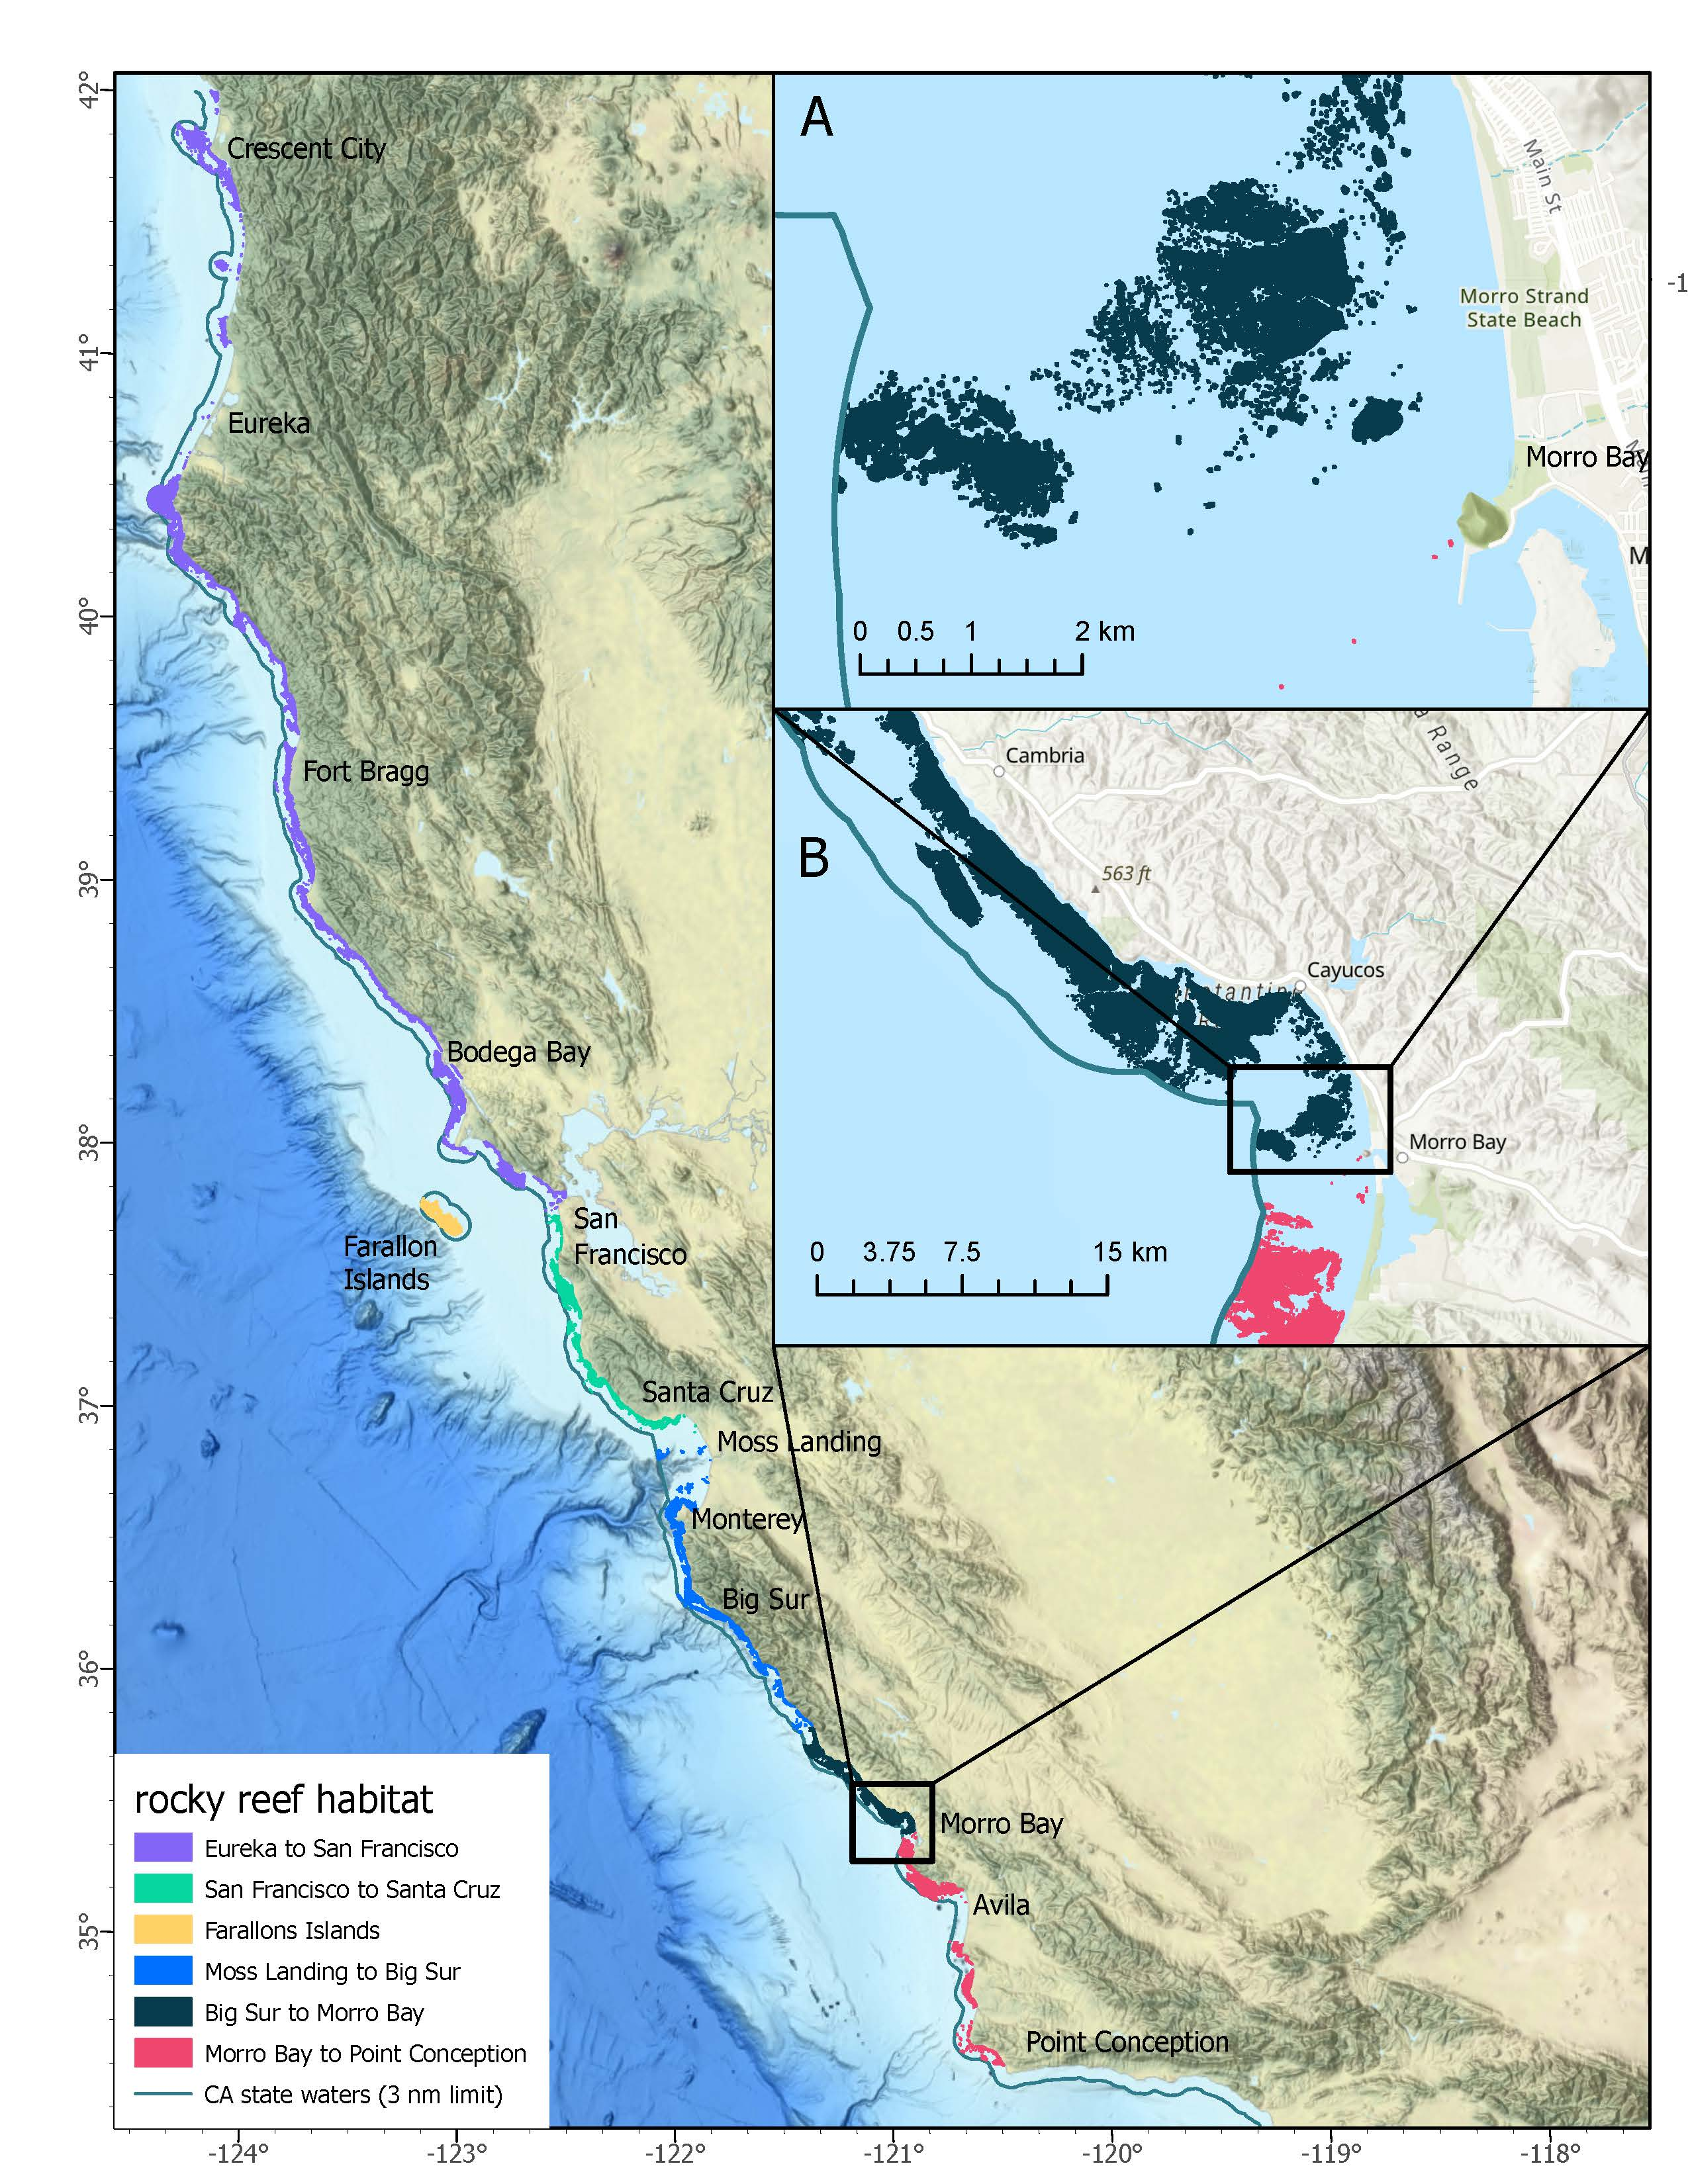
\includegraphics{figures/map.jpg}
\includegraphics{figures/percentpositives_map.jpg}

\begin{figure}

{\centering 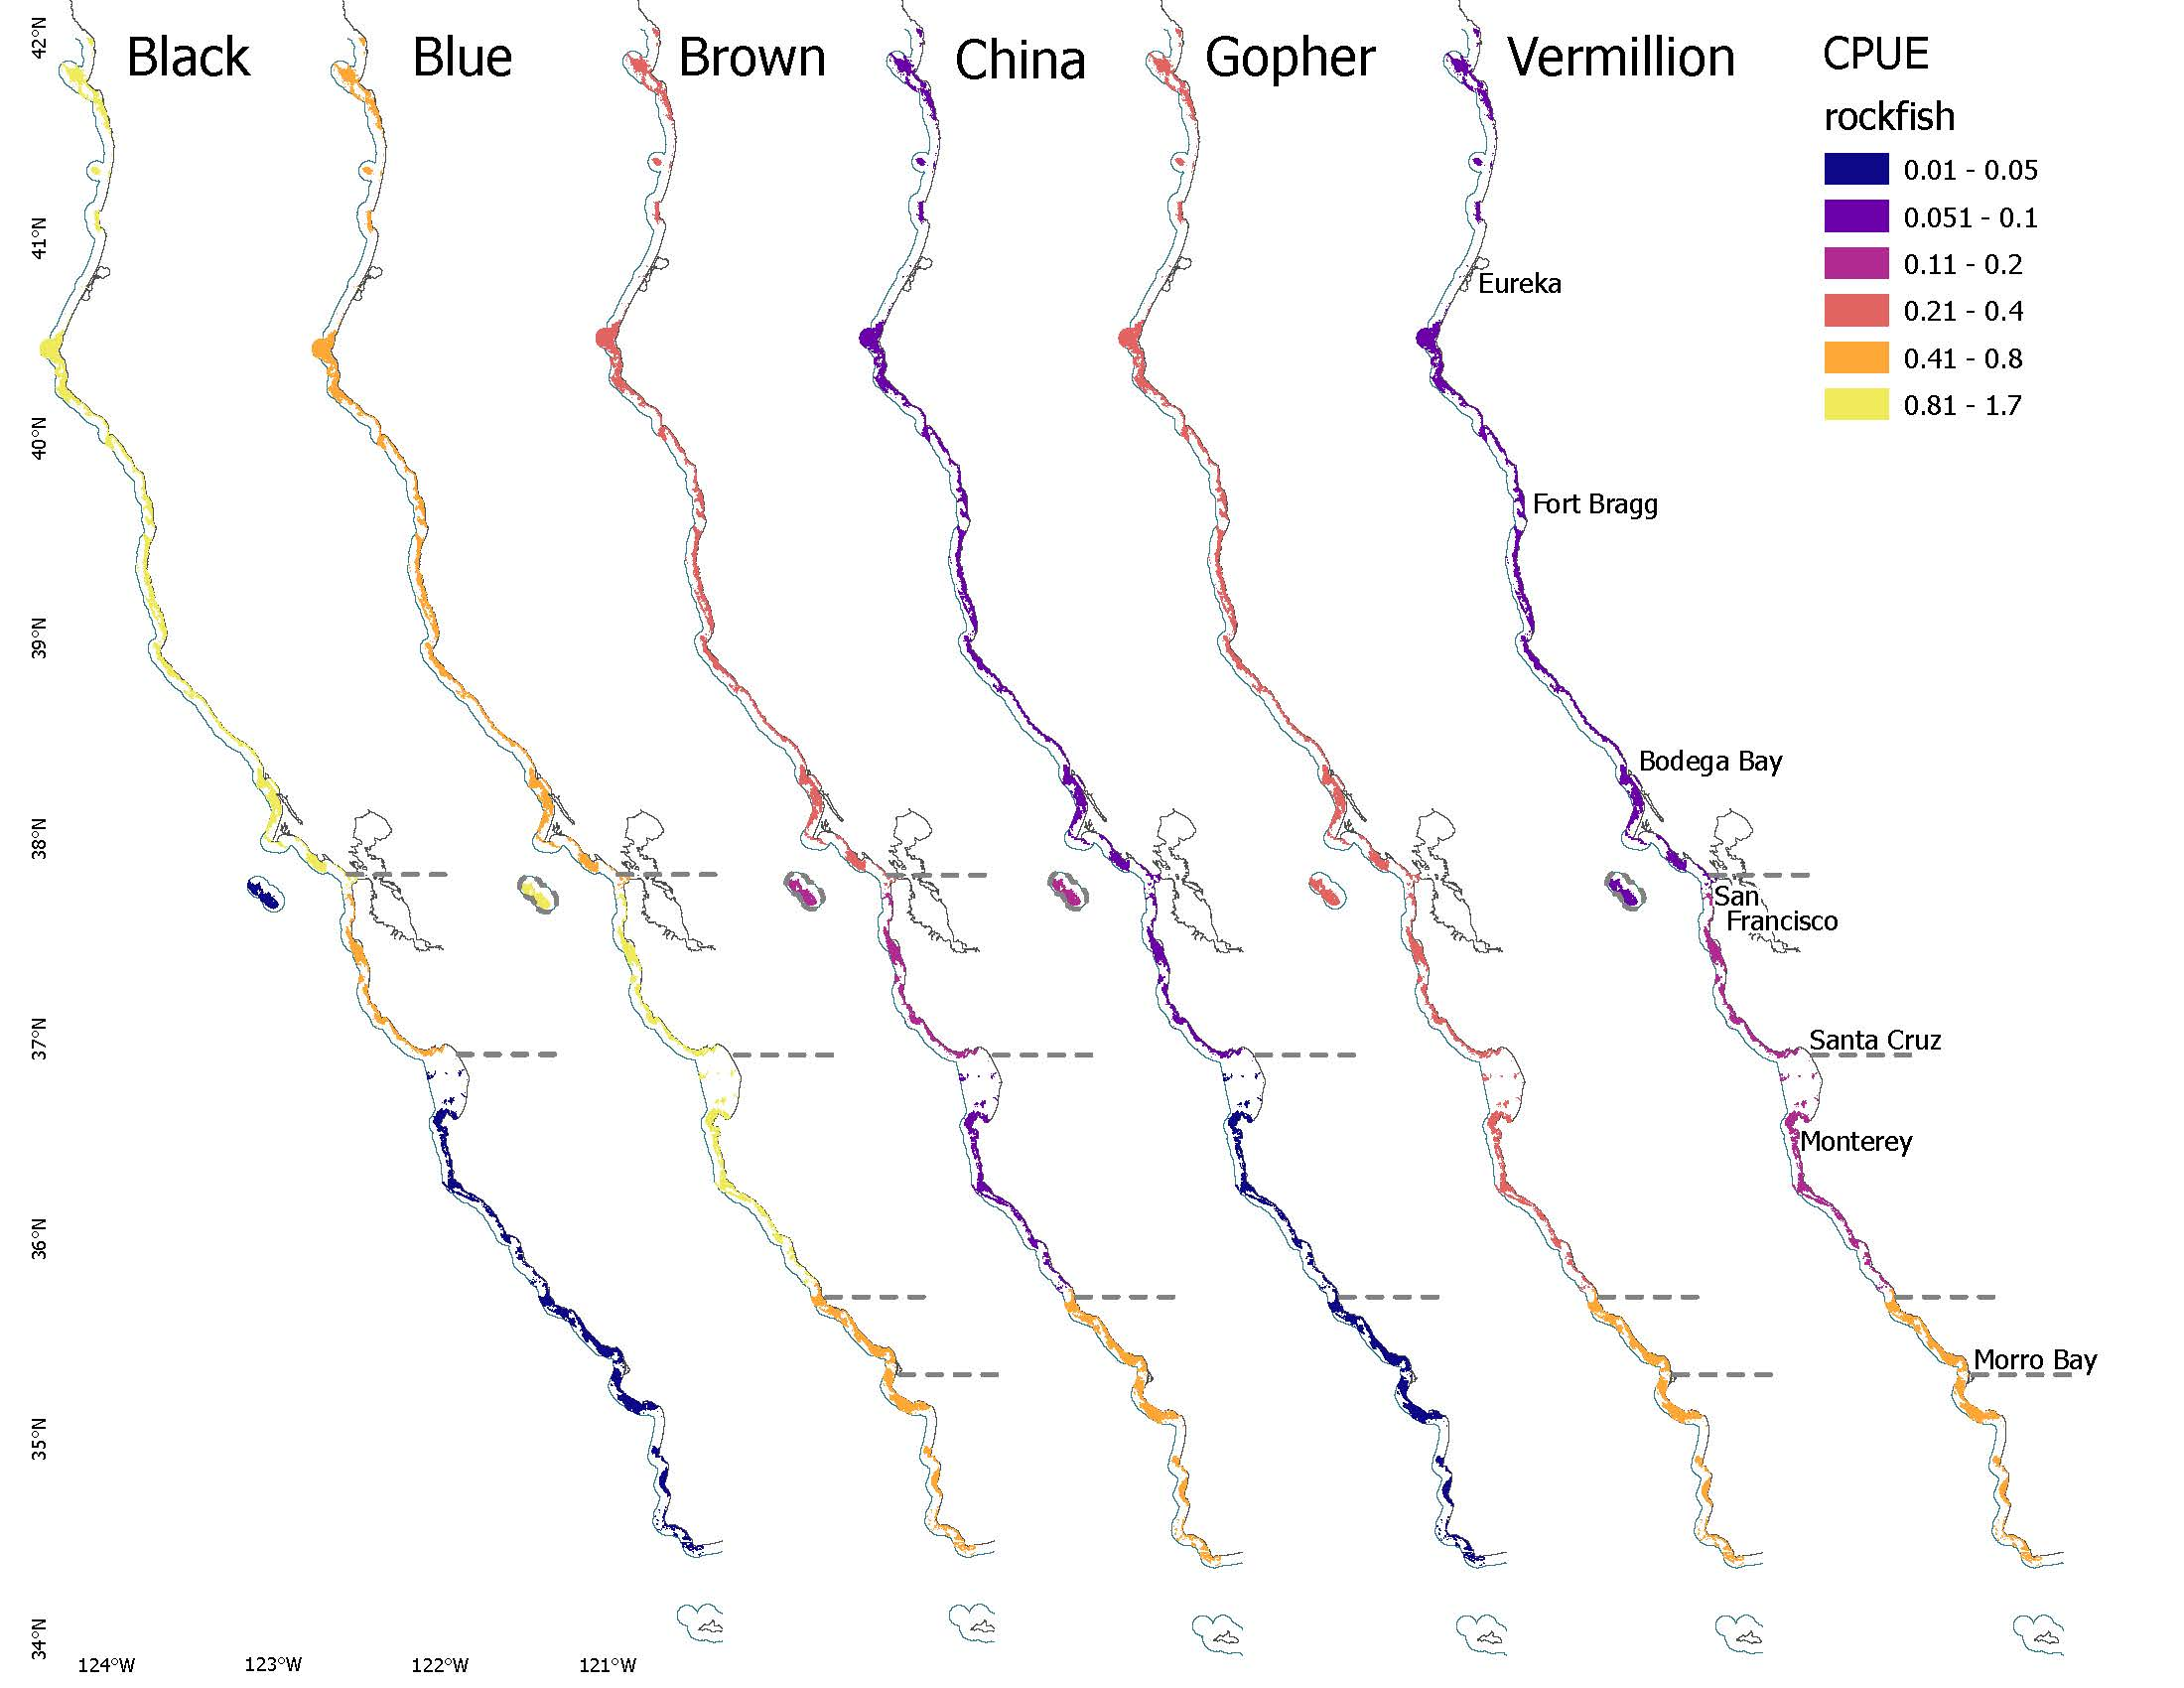
\includegraphics{figures/CPUE_map.jpg}

}

\caption{The average CPUE across all years of the time series for each
of the six species. The grey dashed lines represent the aggregated rocky
habitat used to develop an index of abundance.}

\end{figure}

\begin{figure}

\begin{minipage}[t]{0.50\linewidth}

{\centering 

\raisebox{-\height}{

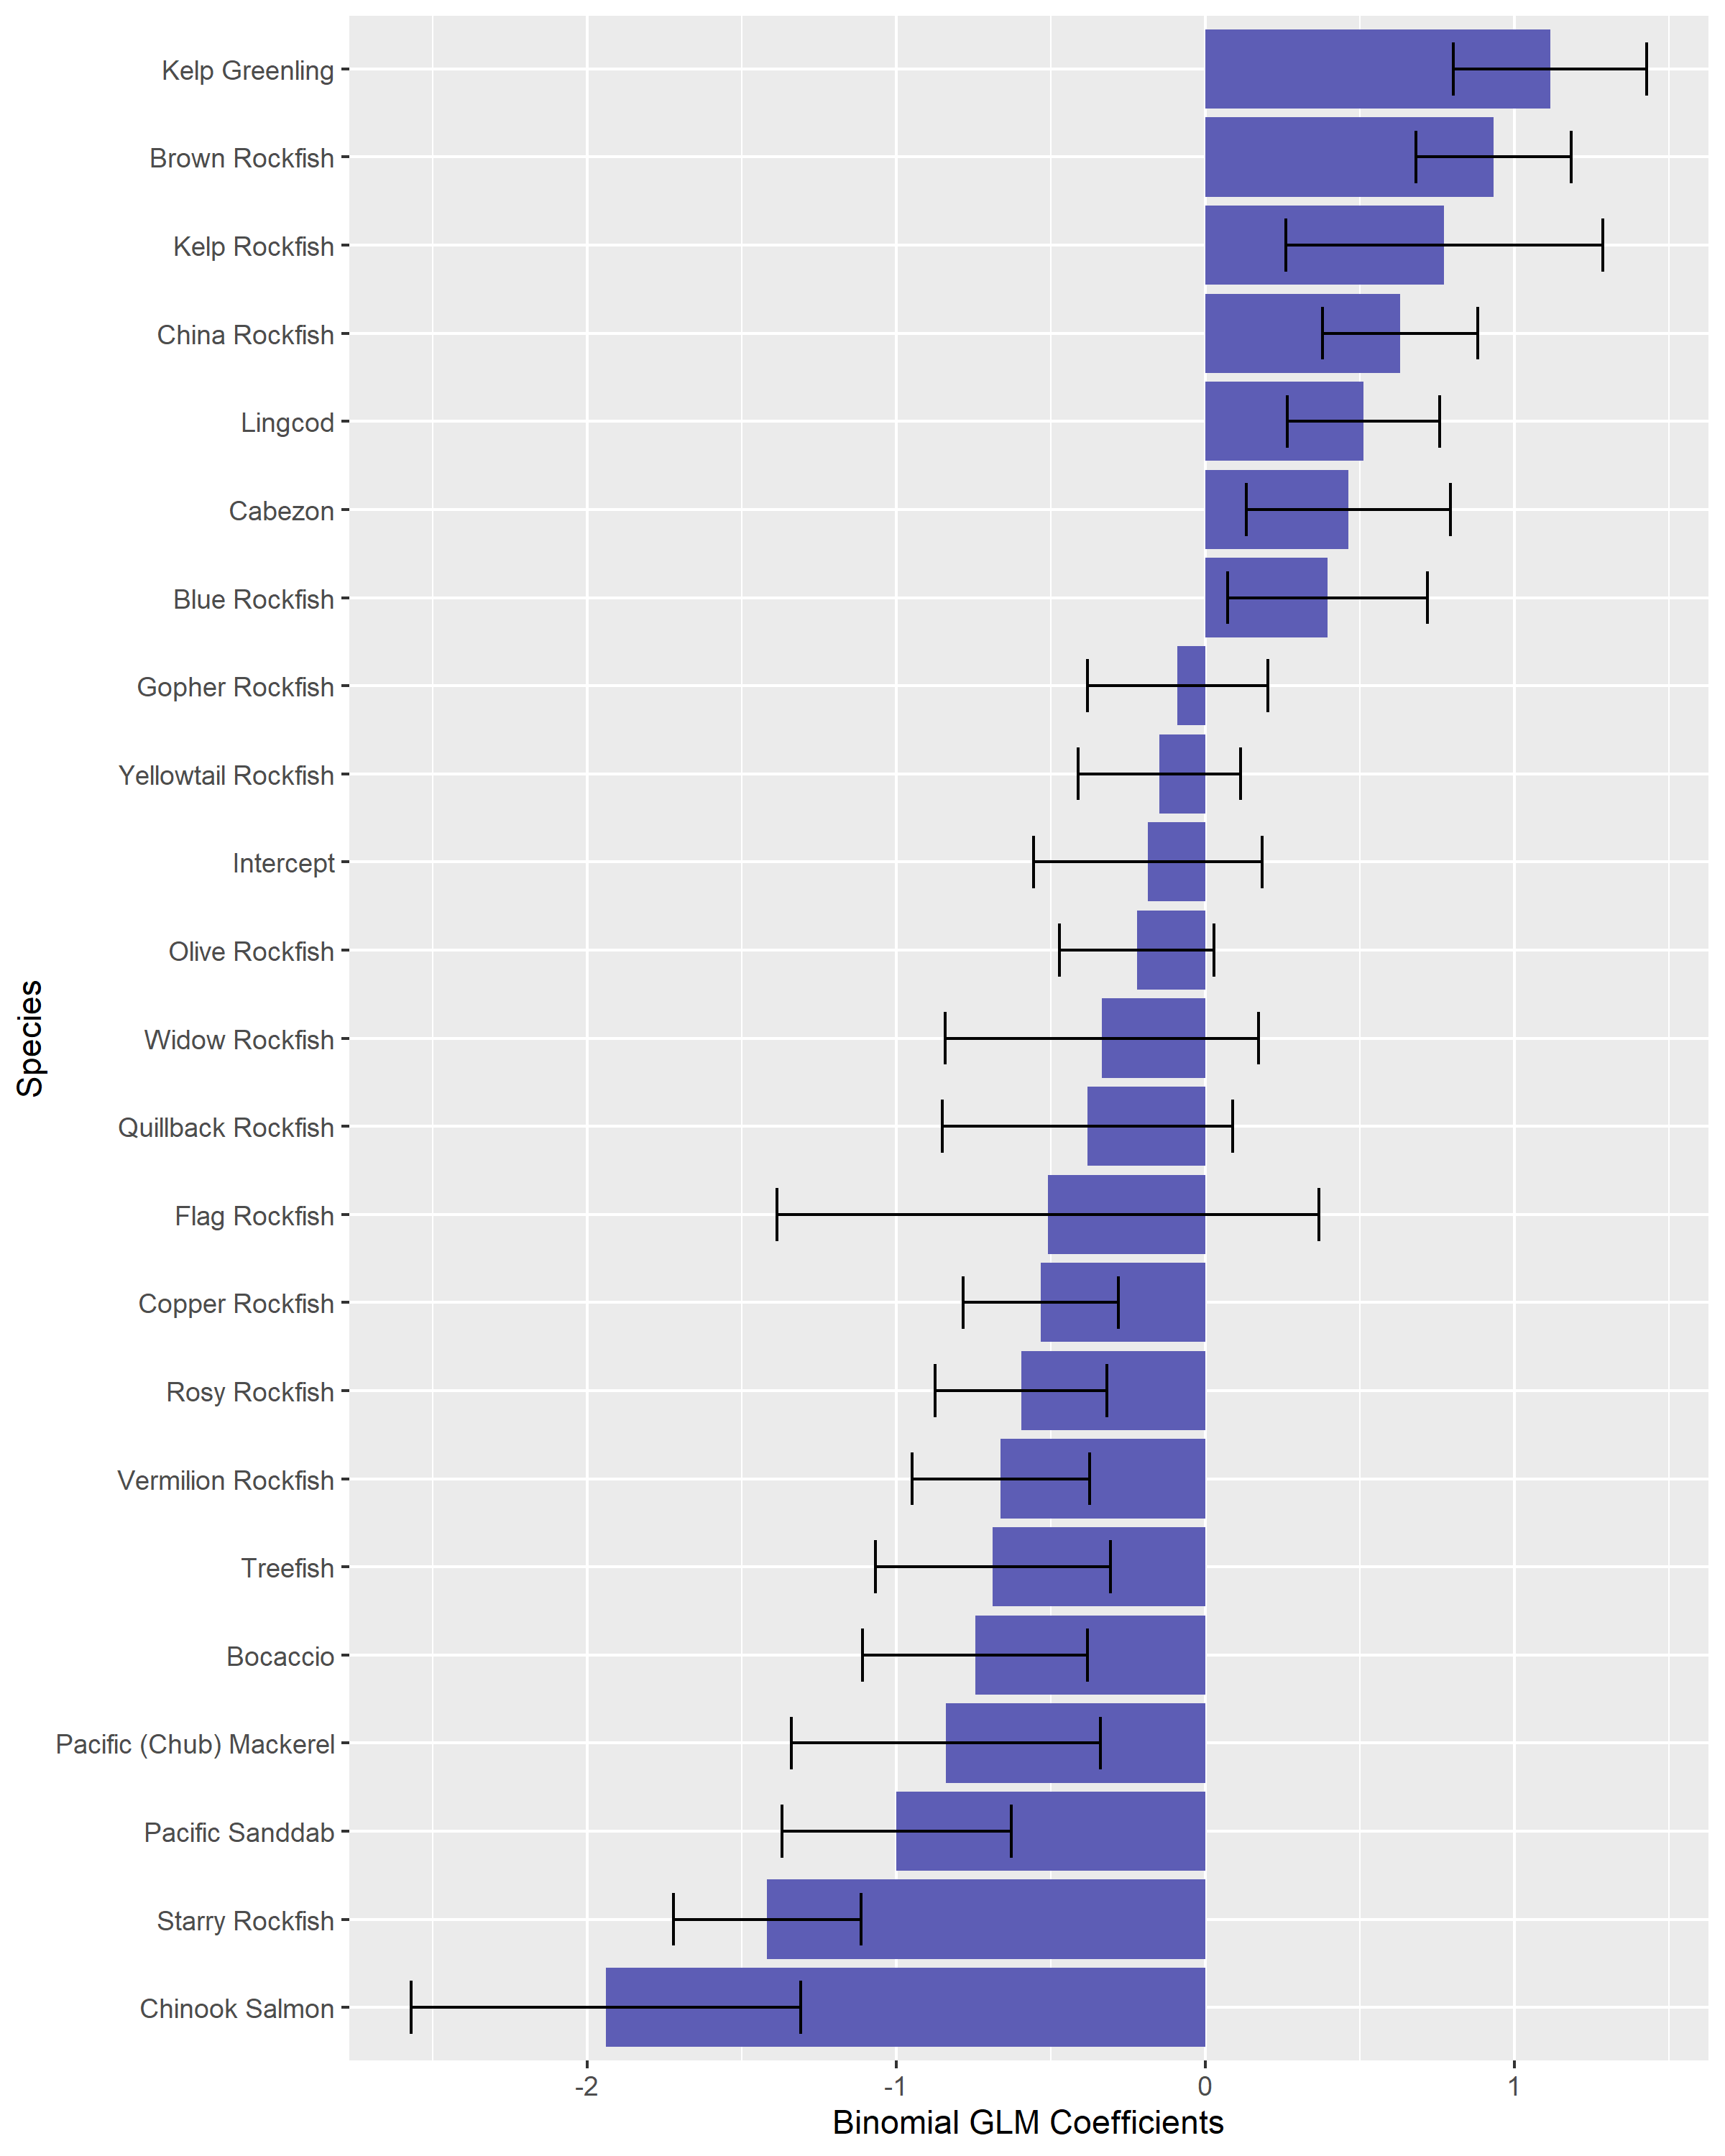
\includegraphics[width=2.75in,height=\textheight]{figures/black_trip_sm.png}

}

}

\subcaption{\label{fig-black-tripsm}Black rockfish trip level}
\end{minipage}%
%
\begin{minipage}[t]{0.50\linewidth}

{\centering 

\raisebox{-\height}{

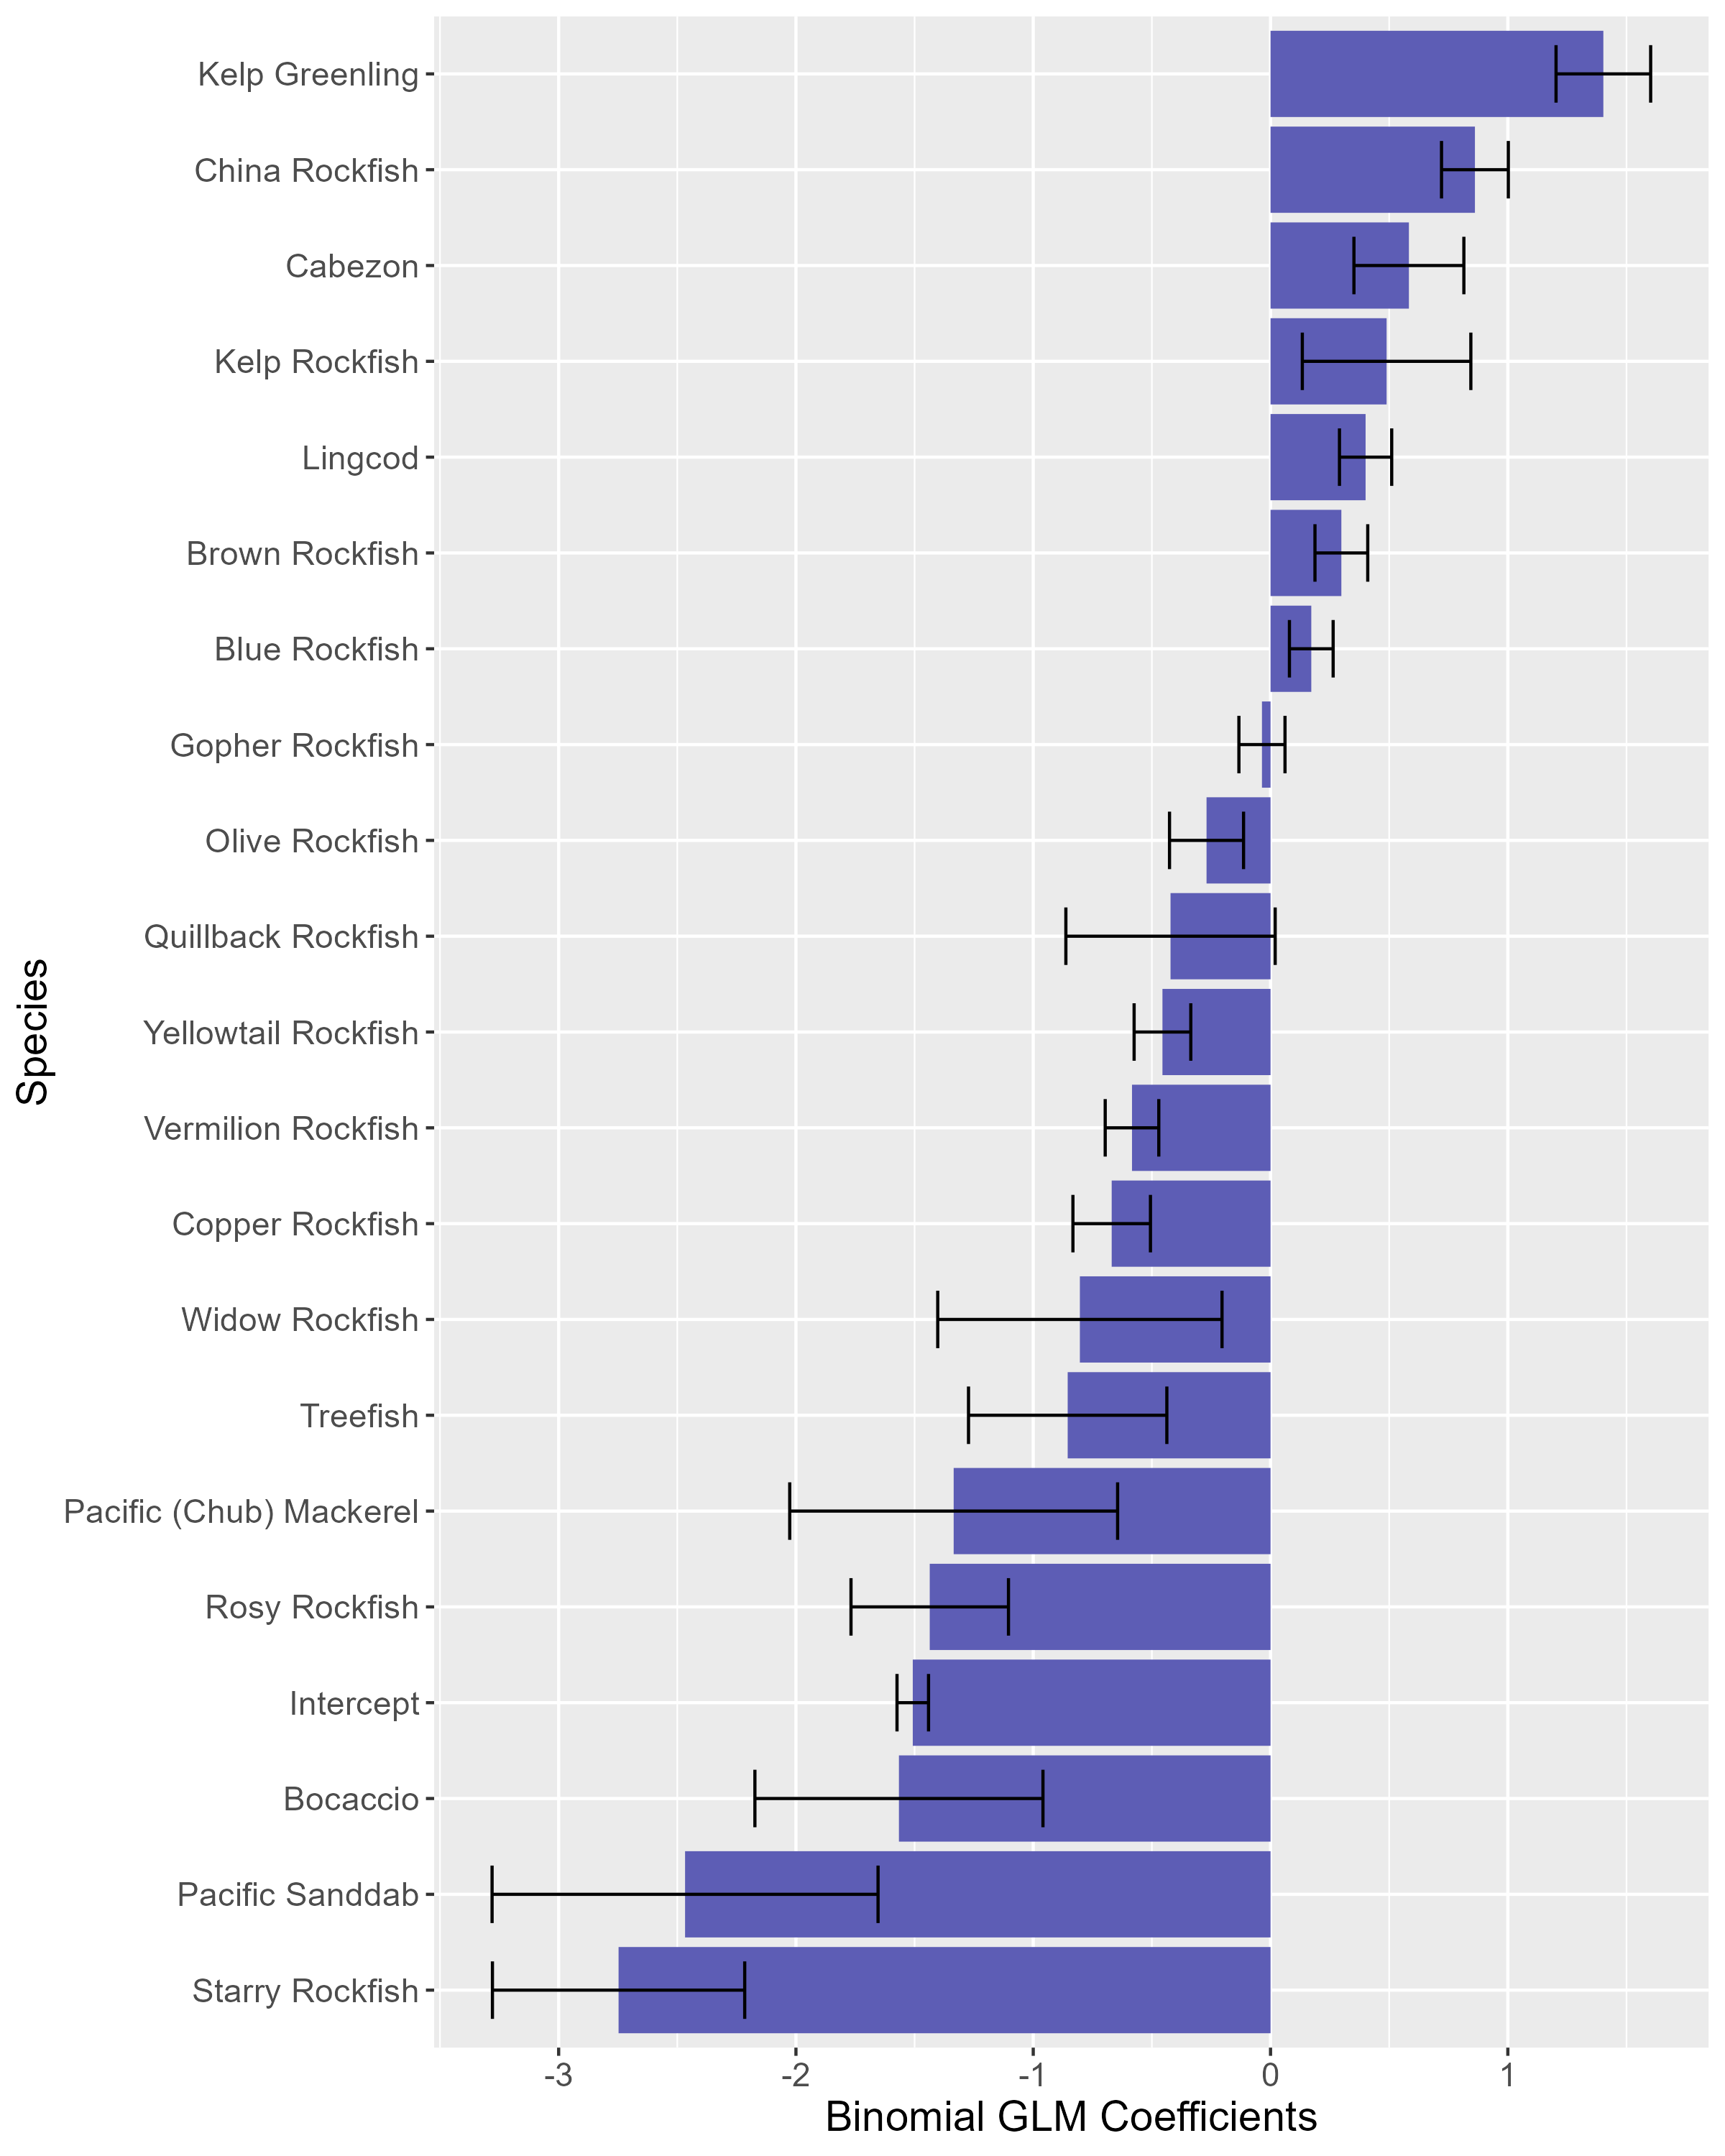
\includegraphics[width=2.75in,height=\textheight]{figures/black_drift_sm.png}

}

}

\subcaption{\label{fig-black-driftsm}Black rockfish drift level}
\end{minipage}%
\newline
\begin{minipage}[t]{0.50\linewidth}

{\centering 

\raisebox{-\height}{

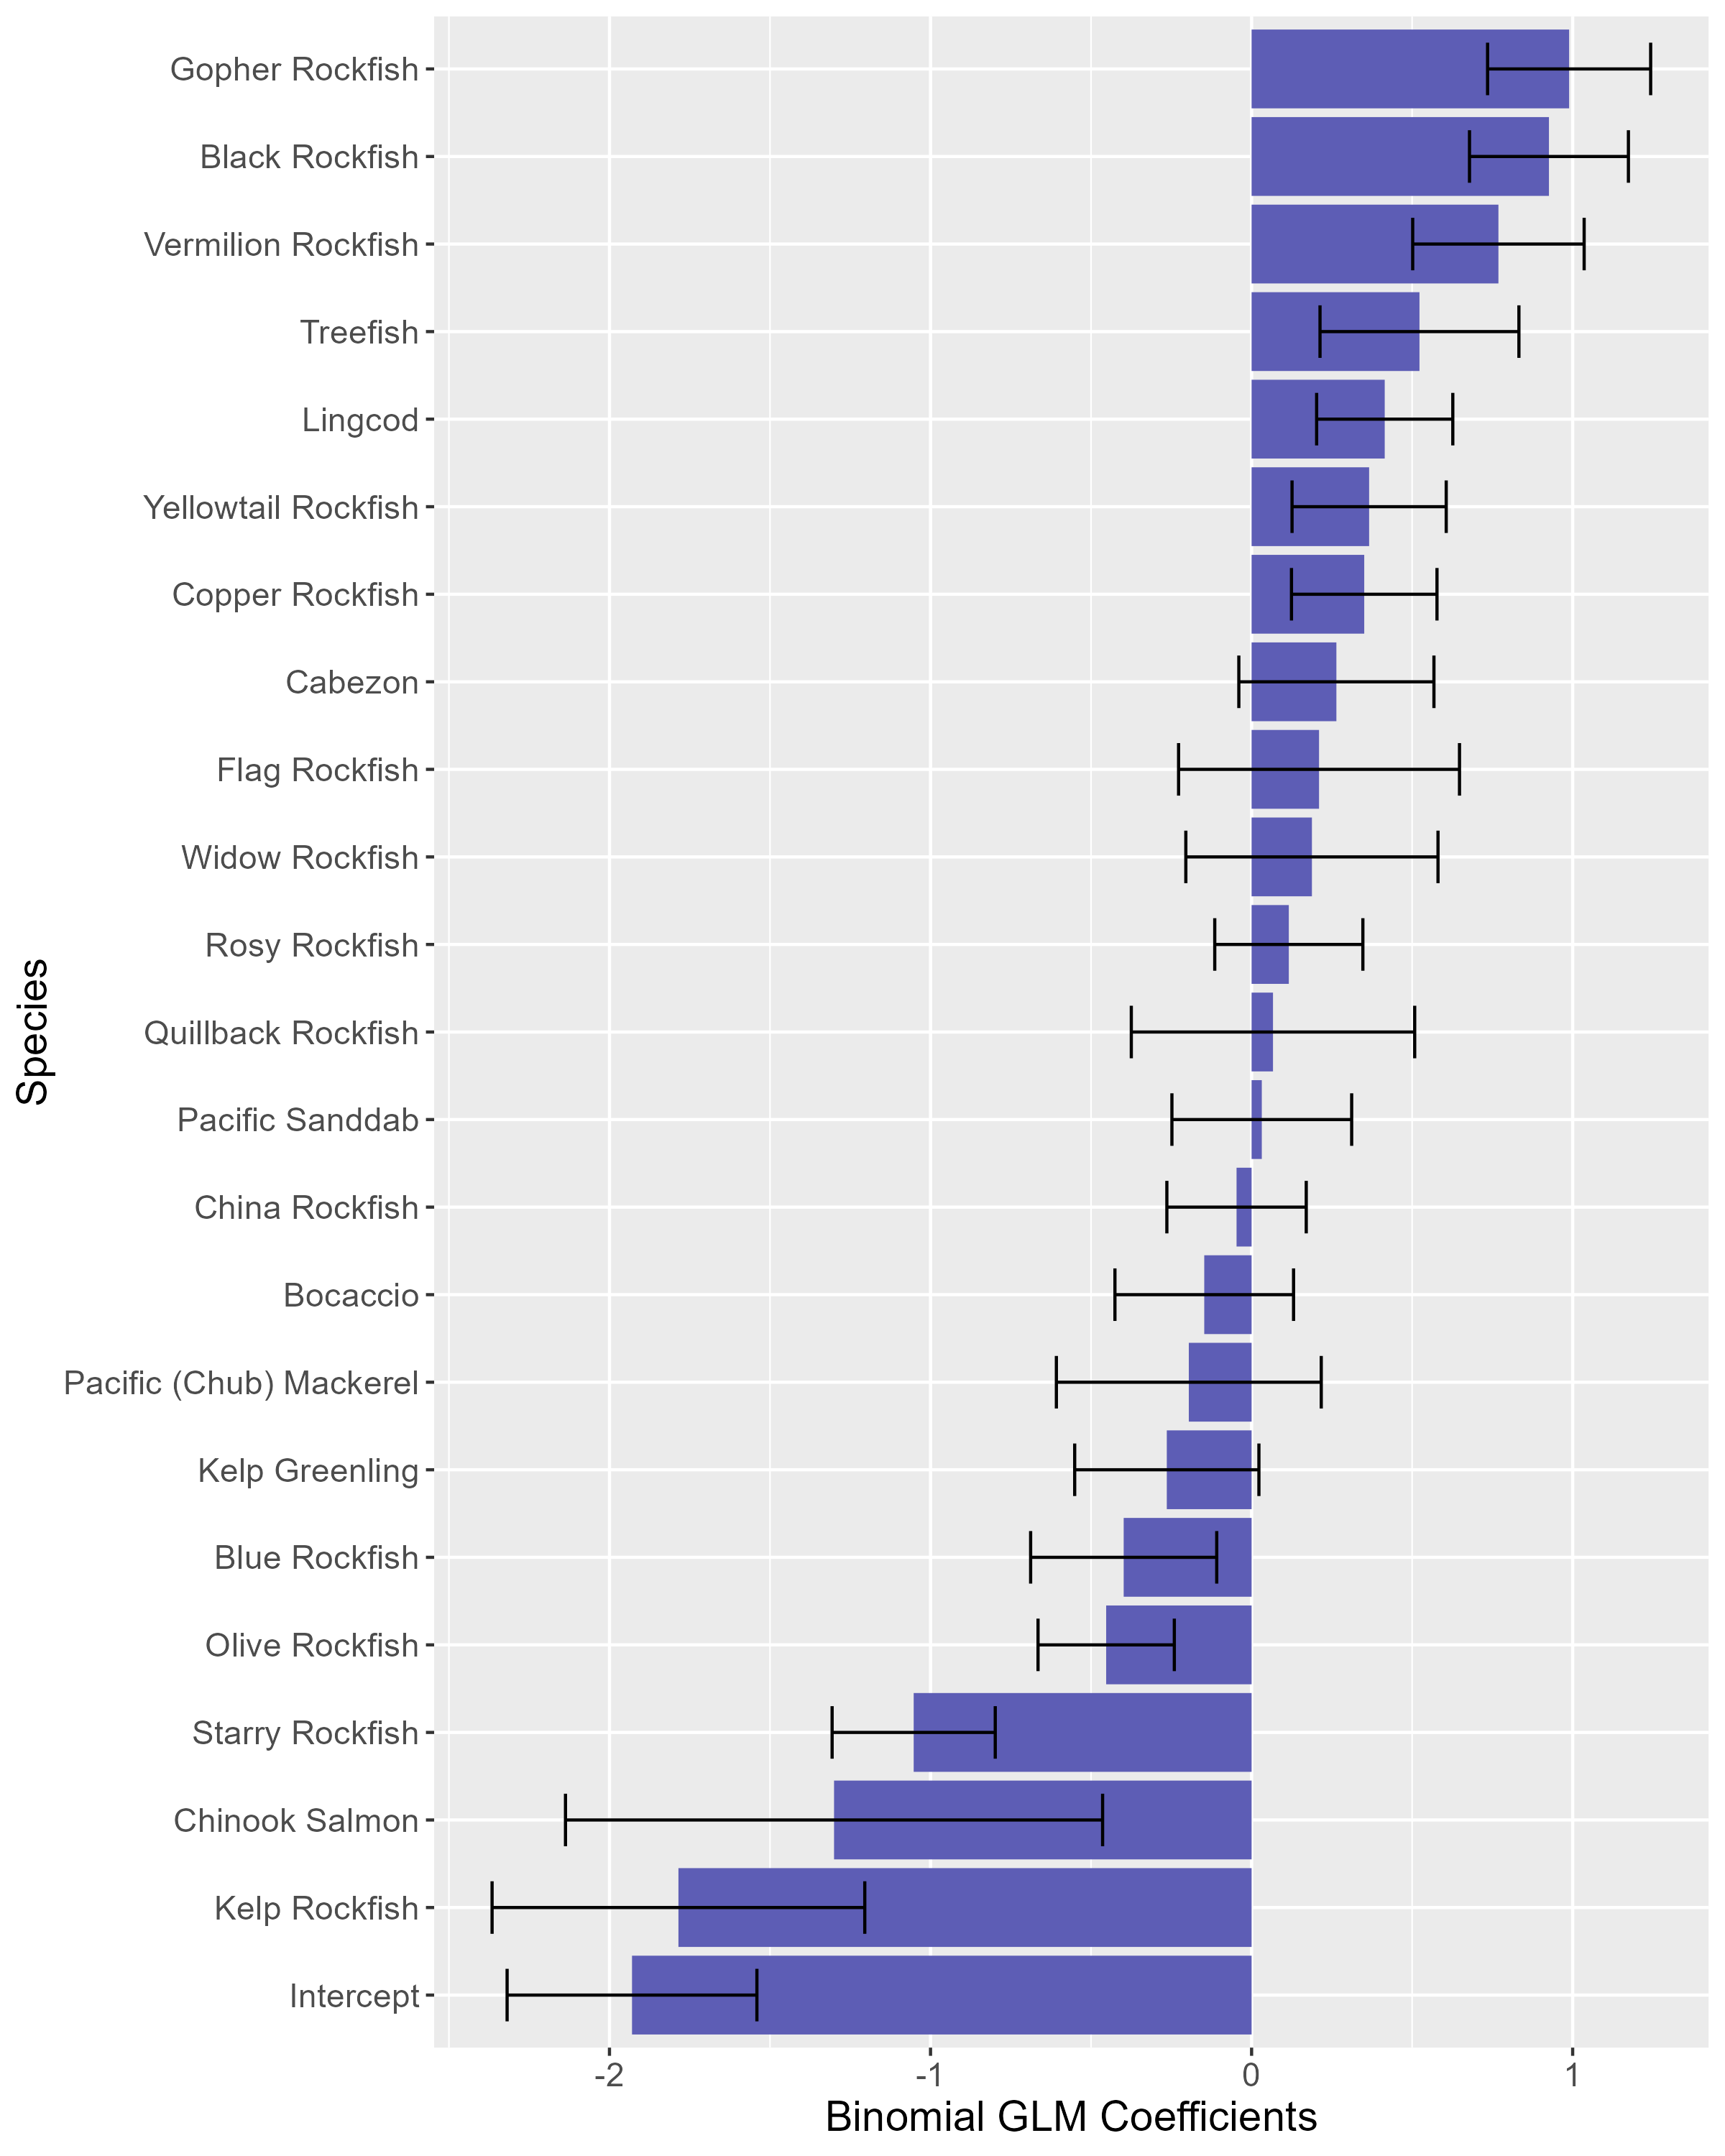
\includegraphics[width=2.75in,height=\textheight]{figures/brown_trip_sm.png}

}

}

\subcaption{\label{fig-brown-tripsm}Brown rockfish trip level}
\end{minipage}%

\caption{\label{fig-sm}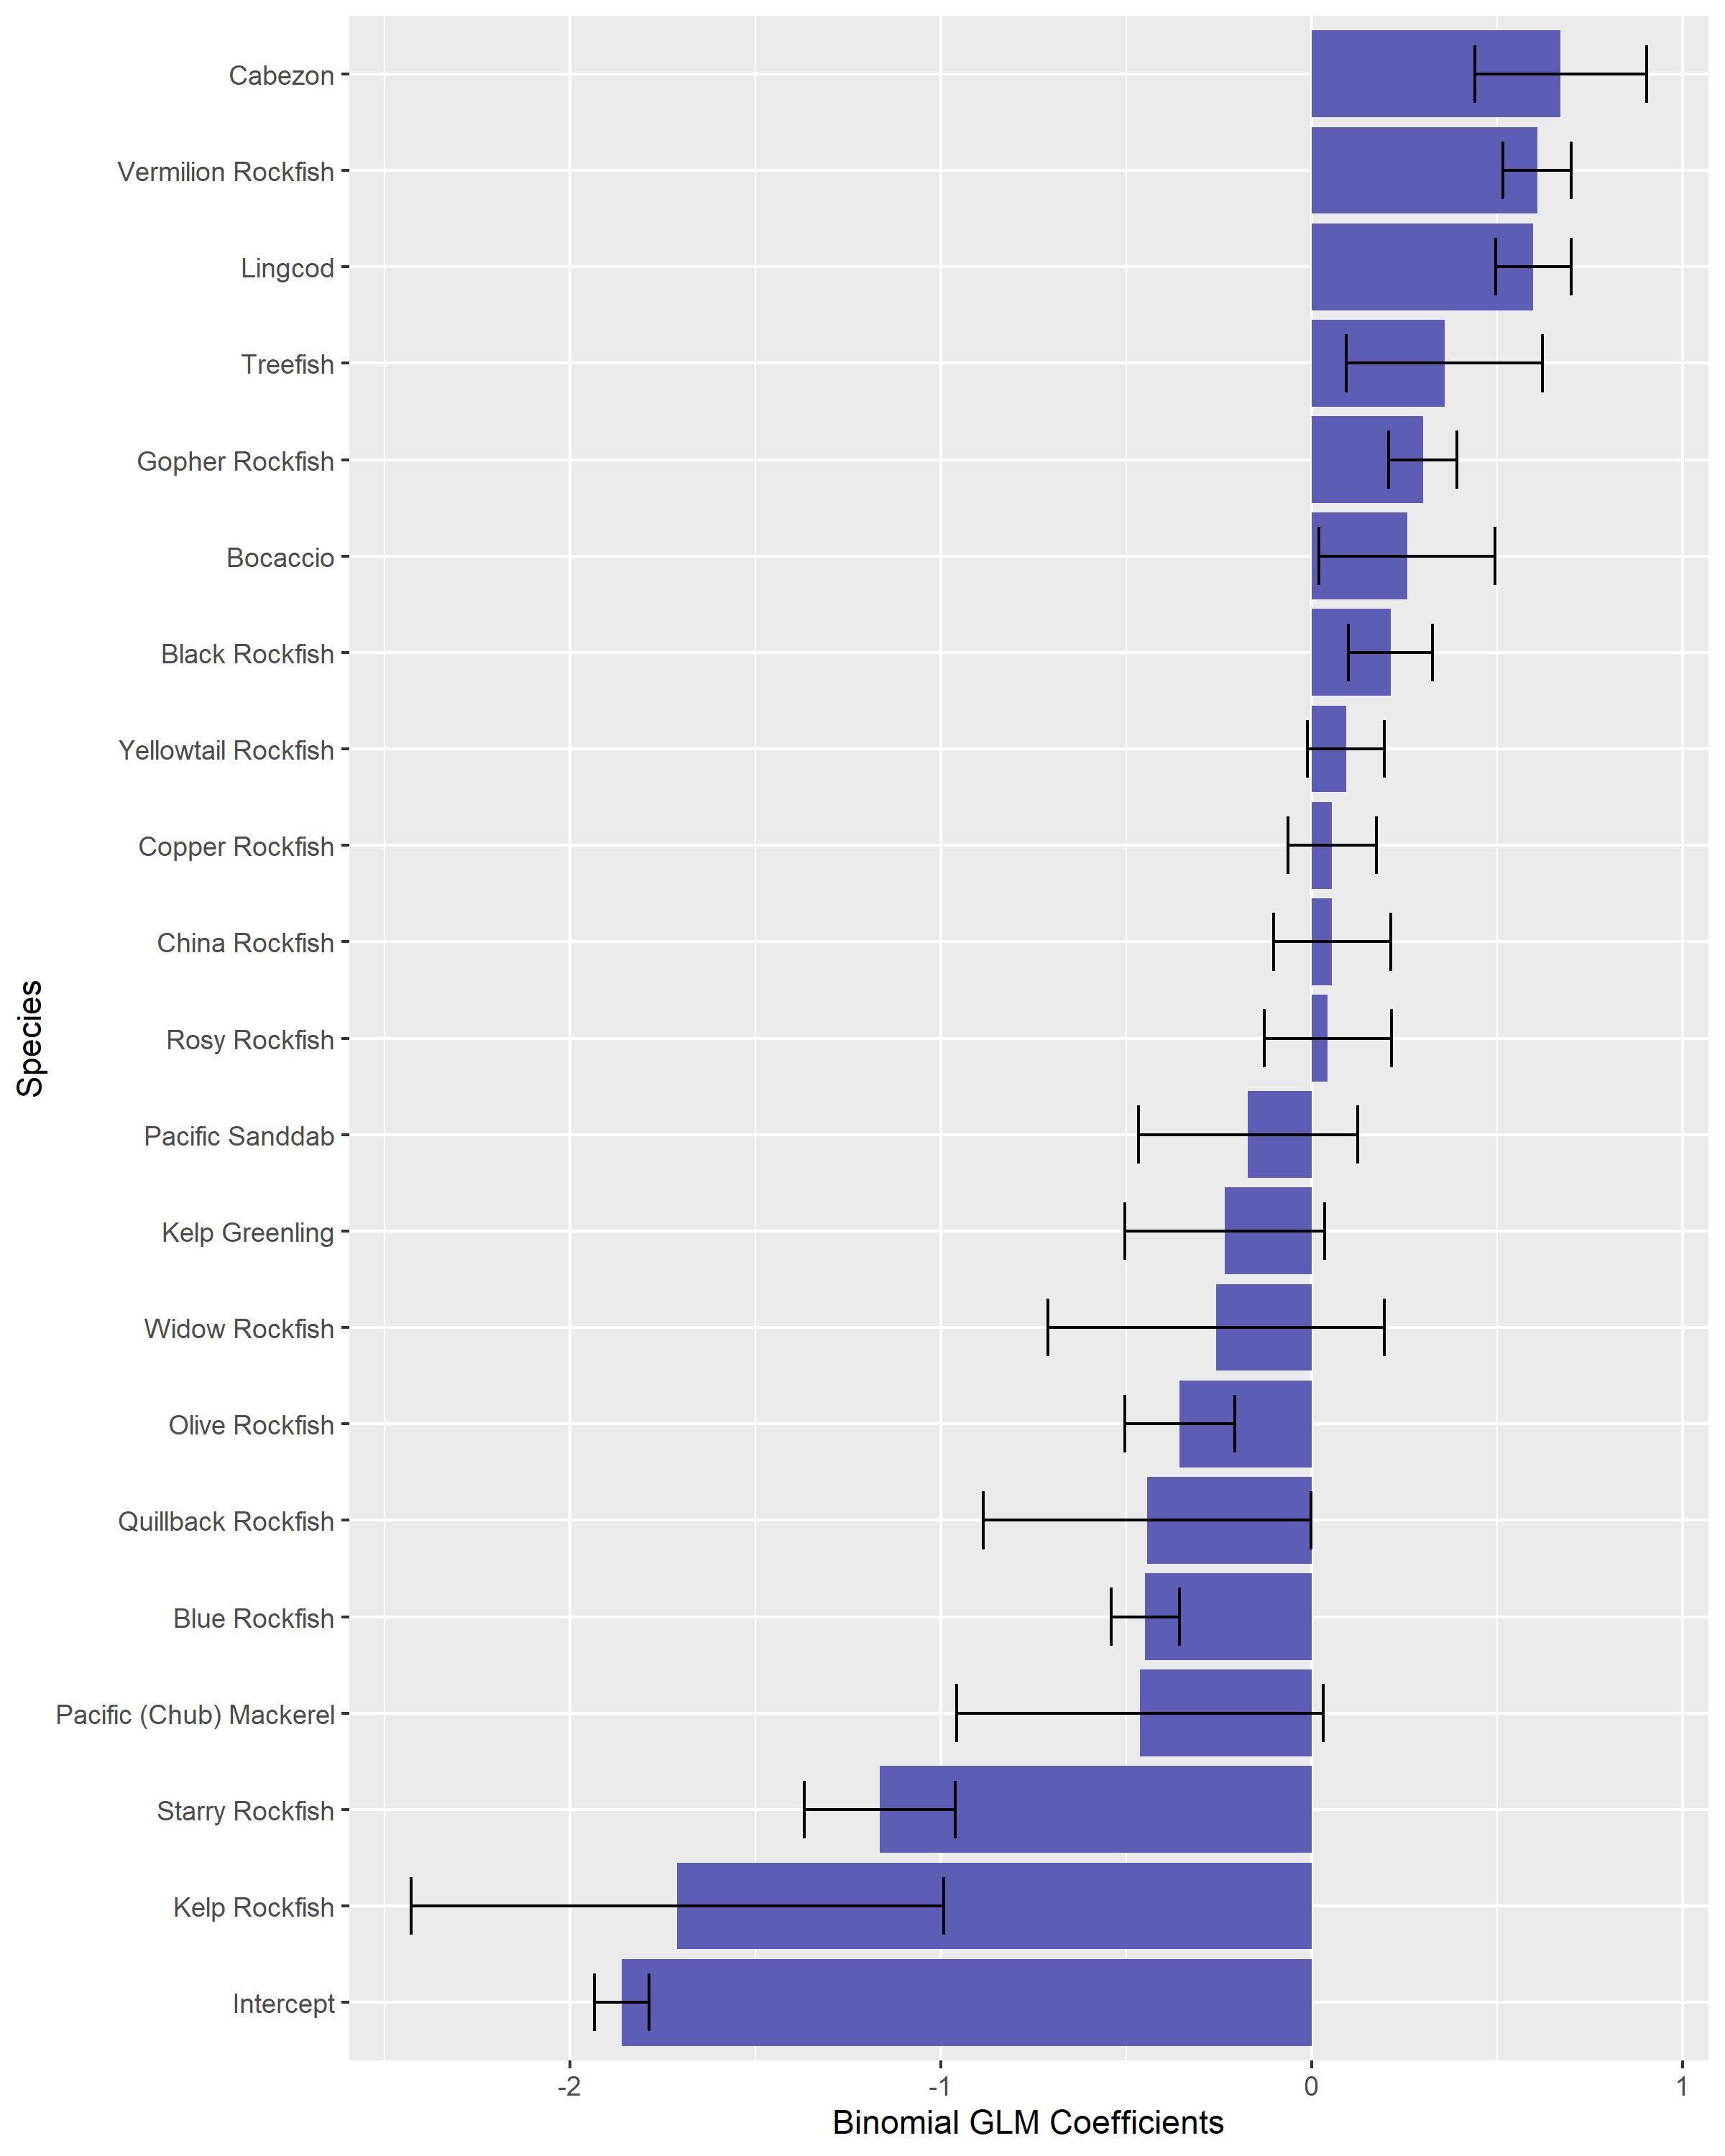
\includegraphics[width=2.75in,height=\textheight]{figures/brown_drift_sm.png}
Examples of the species coefficients for the Stephens-MacCall filtering
for two species using the trip-level and drift-level data.}

\end{figure}

\begin{figure}

\begin{minipage}[t]{0.50\linewidth}

{\centering 

\raisebox{-\height}{

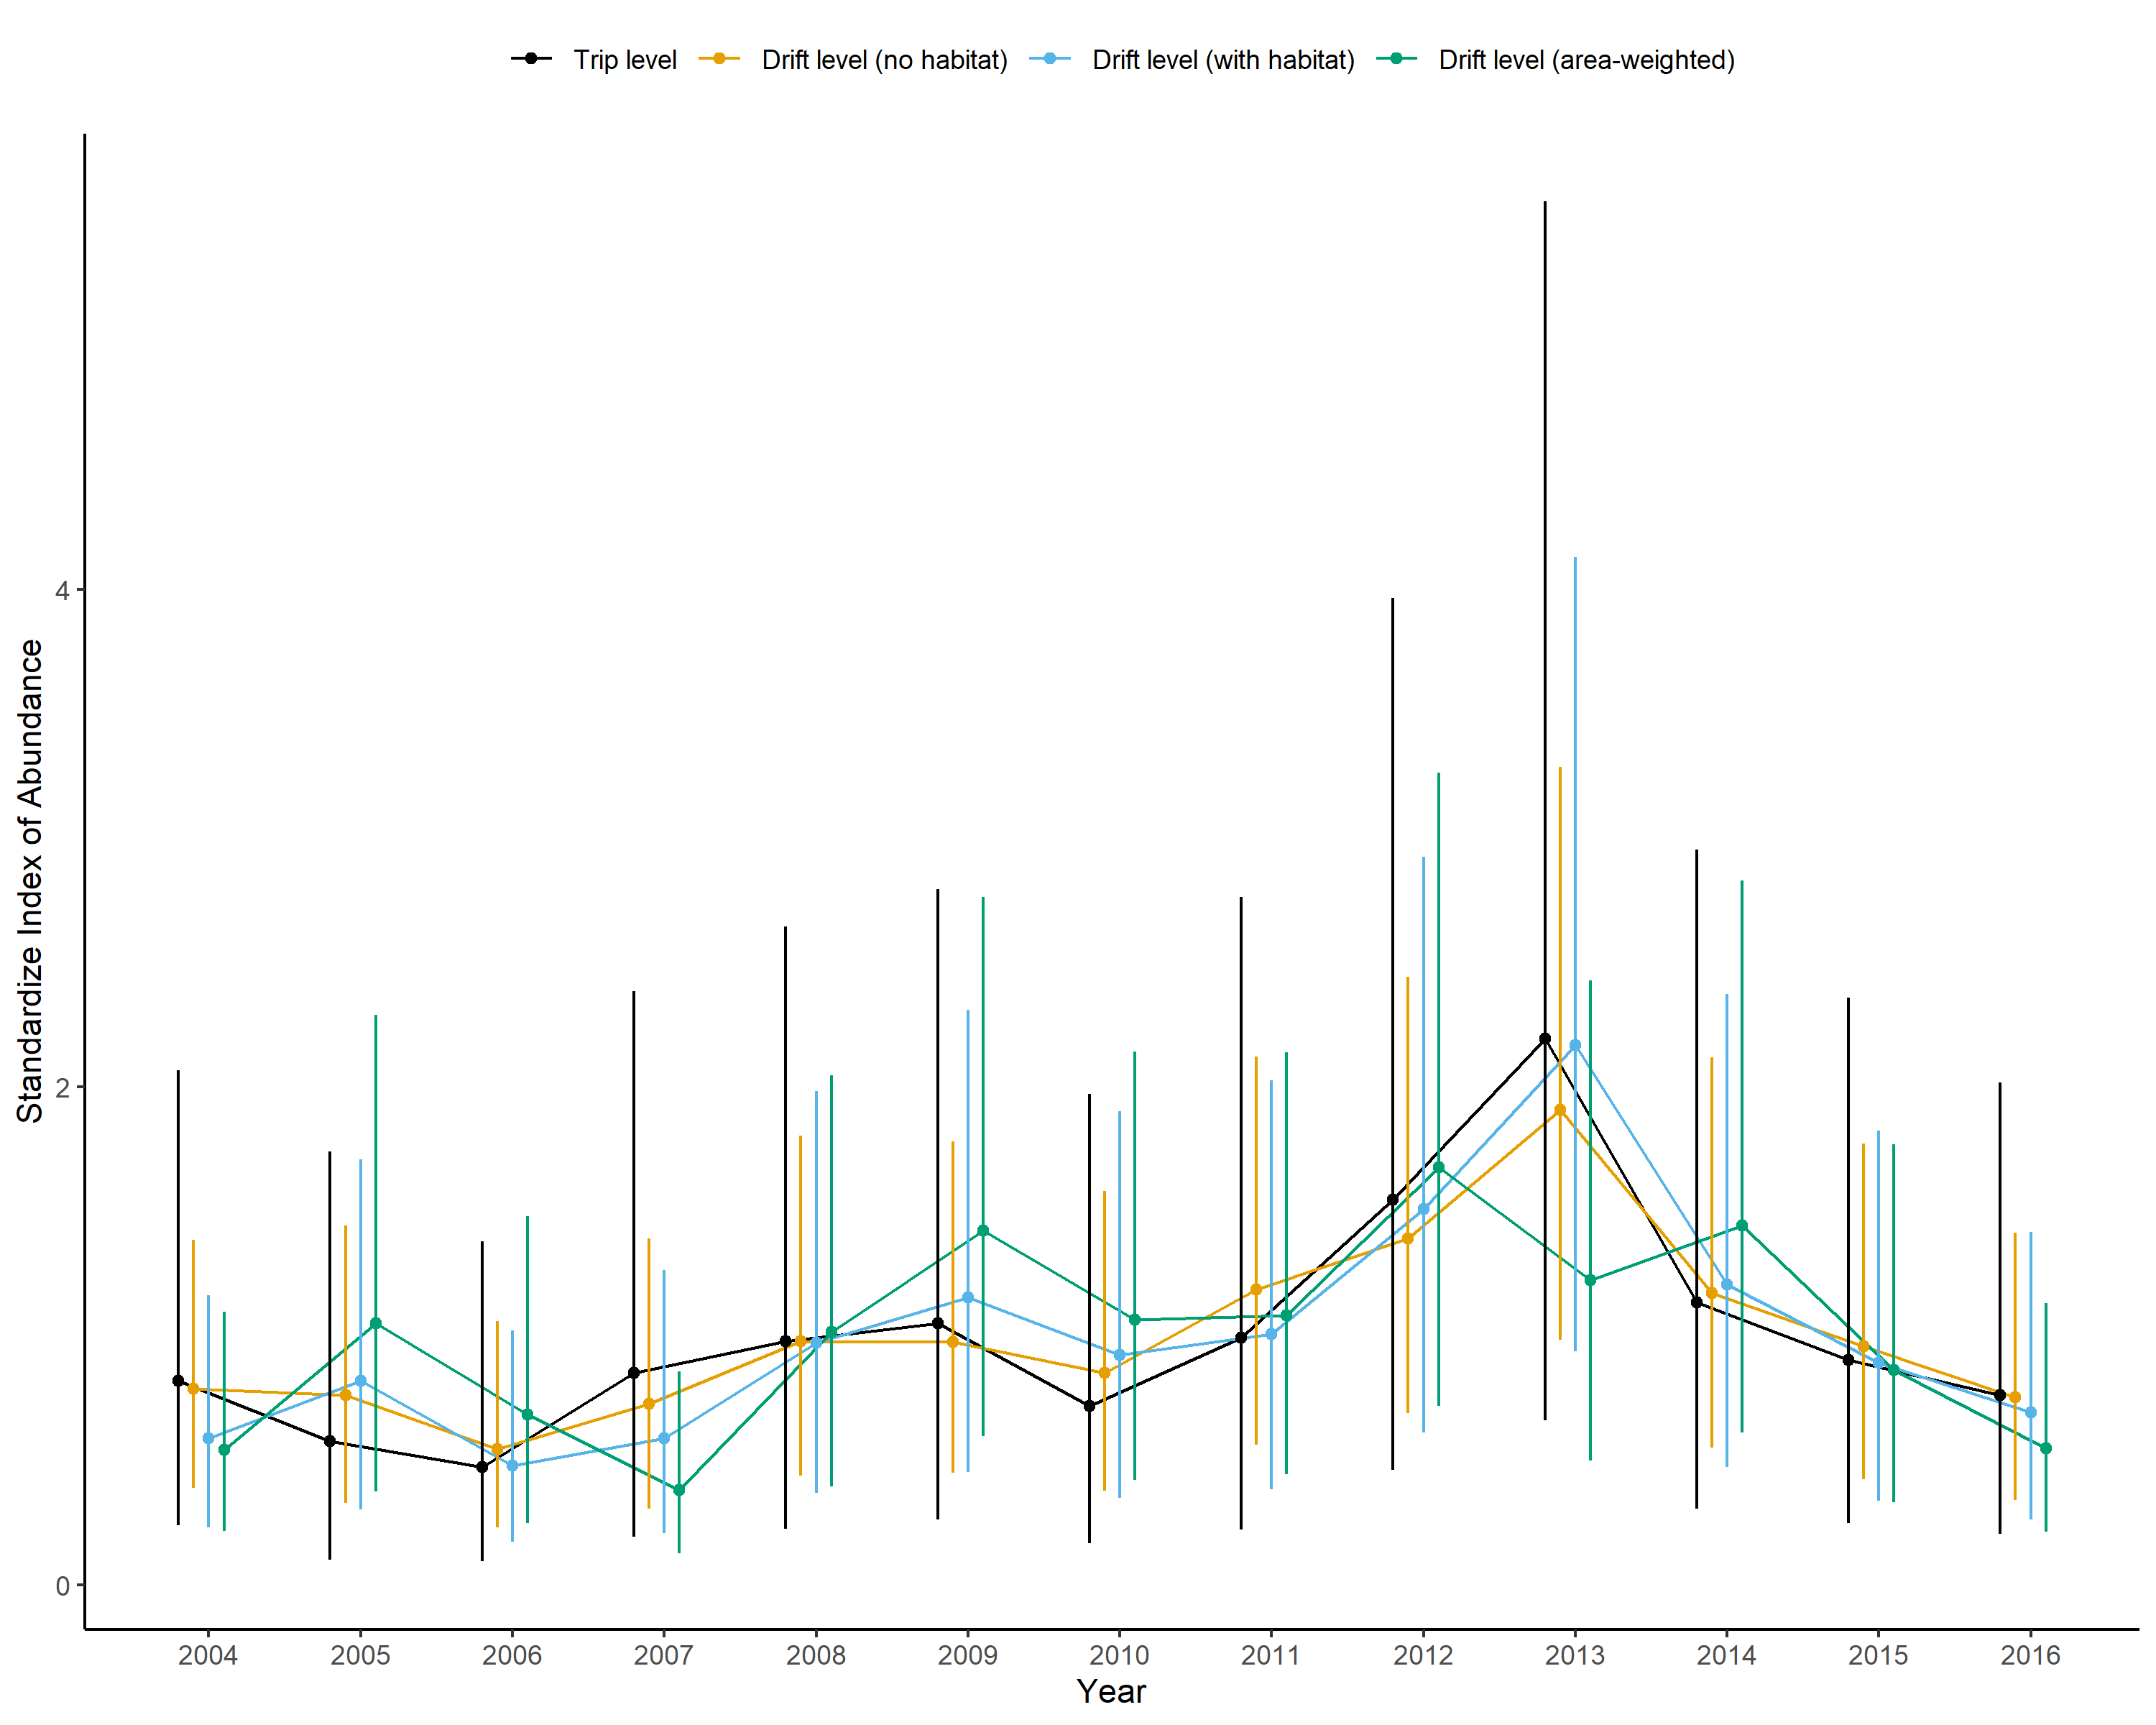
\includegraphics[width=3in,height=\textheight]{figures/black_indices.png}

}

\caption{\label{fig-black-indices}Black rockfish}

}

\end{minipage}%
%
\begin{minipage}[t]{0.50\linewidth}

{\centering 

\raisebox{-\height}{

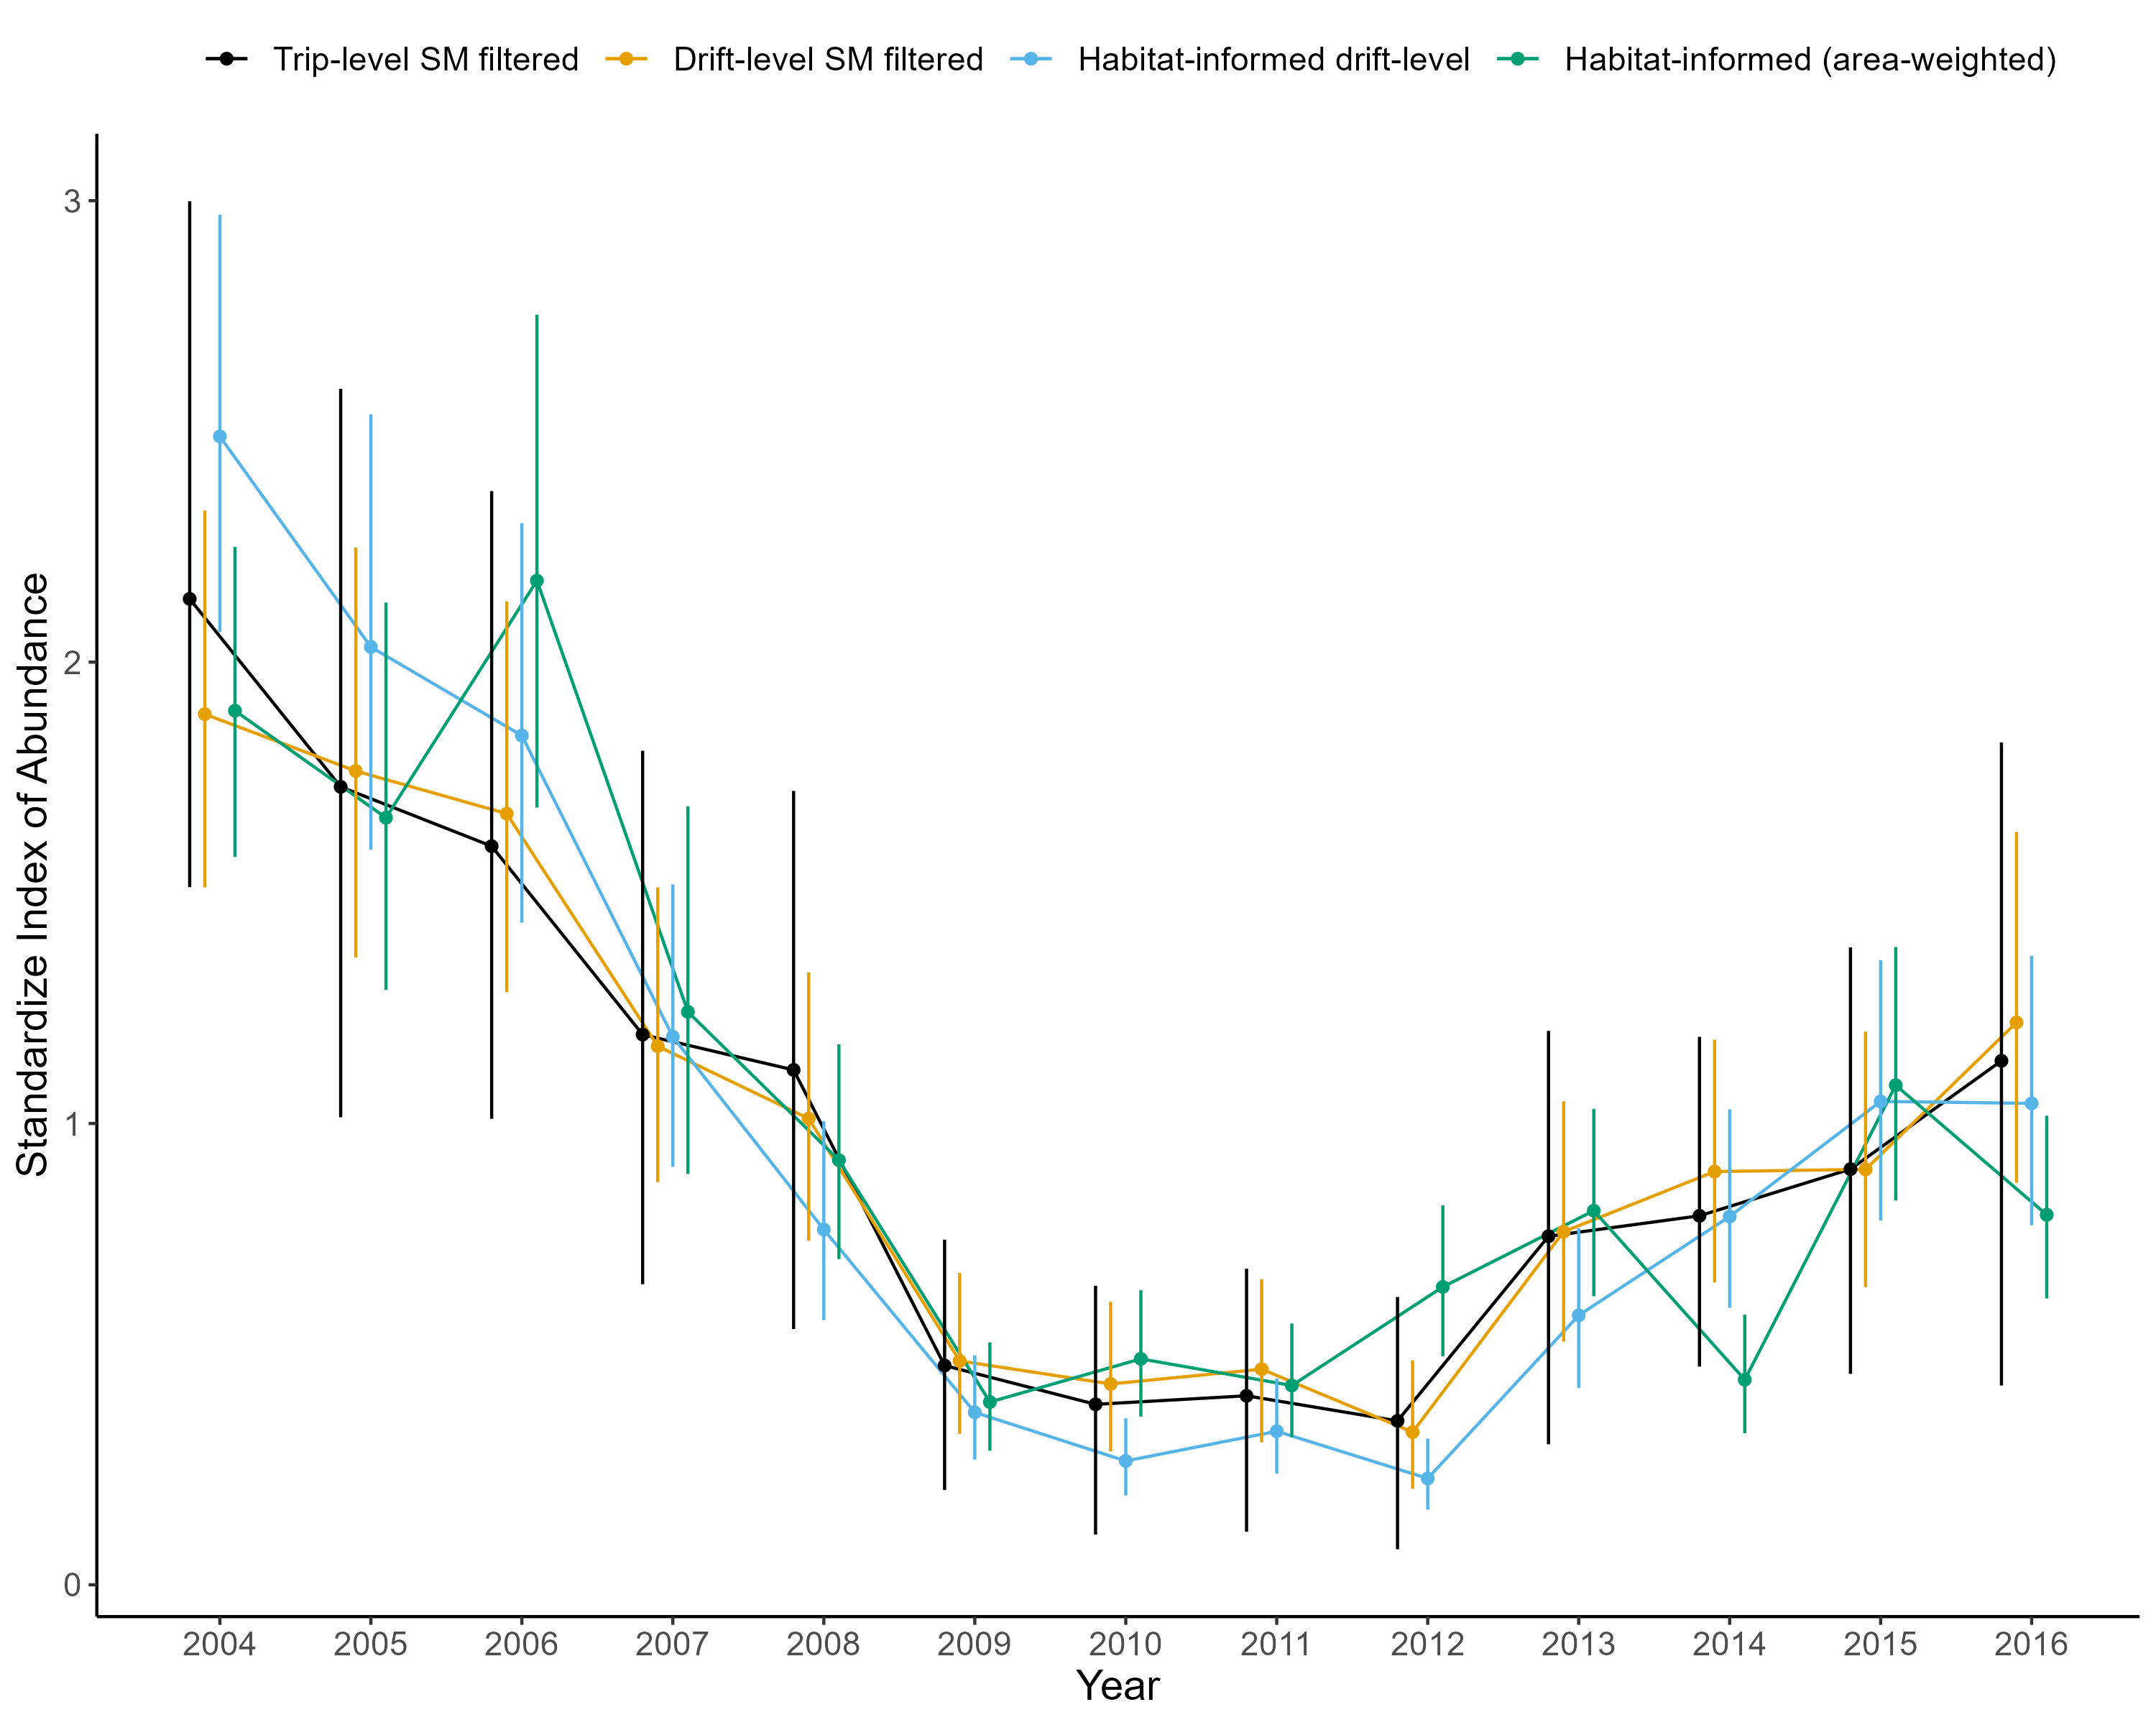
\includegraphics[width=3in,height=\textheight]{figures/blue_indices.png}

}

\caption{\label{fig-blue-indices}Blue rockfish}

}

\end{minipage}%
\newline
\begin{minipage}[t]{0.50\linewidth}

{\centering 

\raisebox{-\height}{

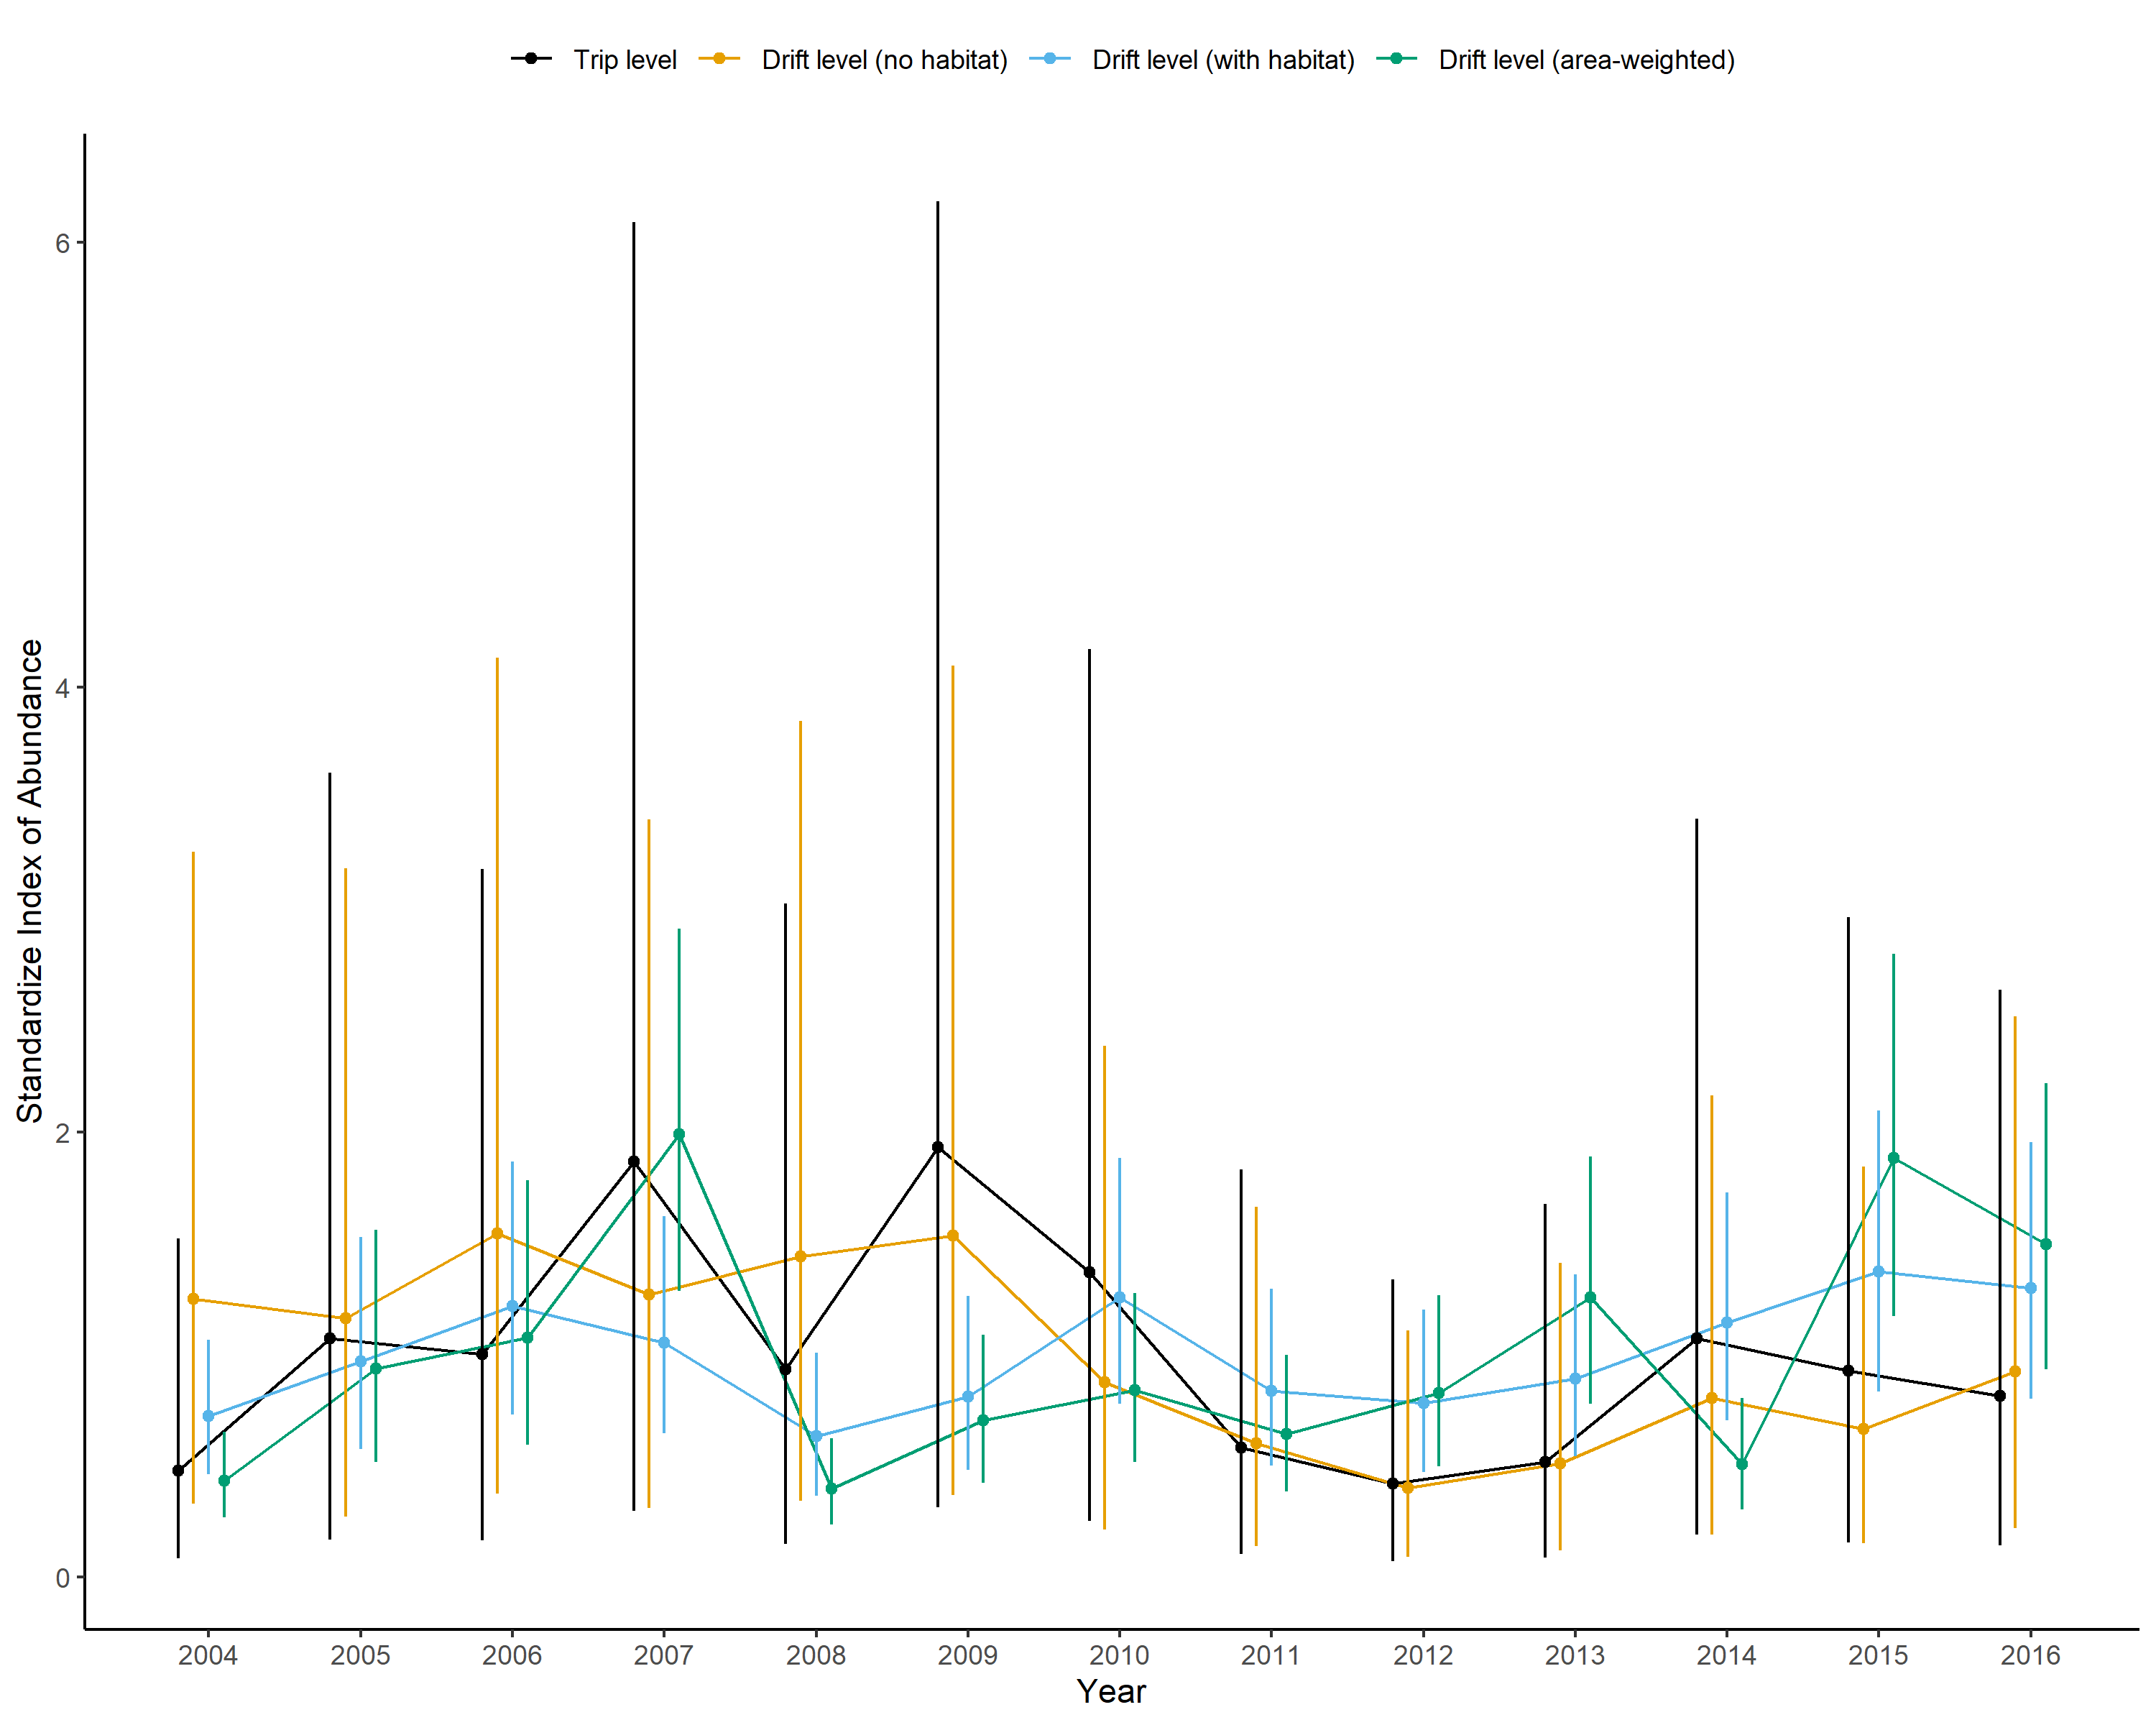
\includegraphics[width=3in,height=\textheight]{figures/brown_indices.png}

}

\caption{\label{fig-brown-indices}Brown rockfish}

}

\end{minipage}%
%
\begin{minipage}[t]{0.50\linewidth}

{\centering 

\raisebox{-\height}{

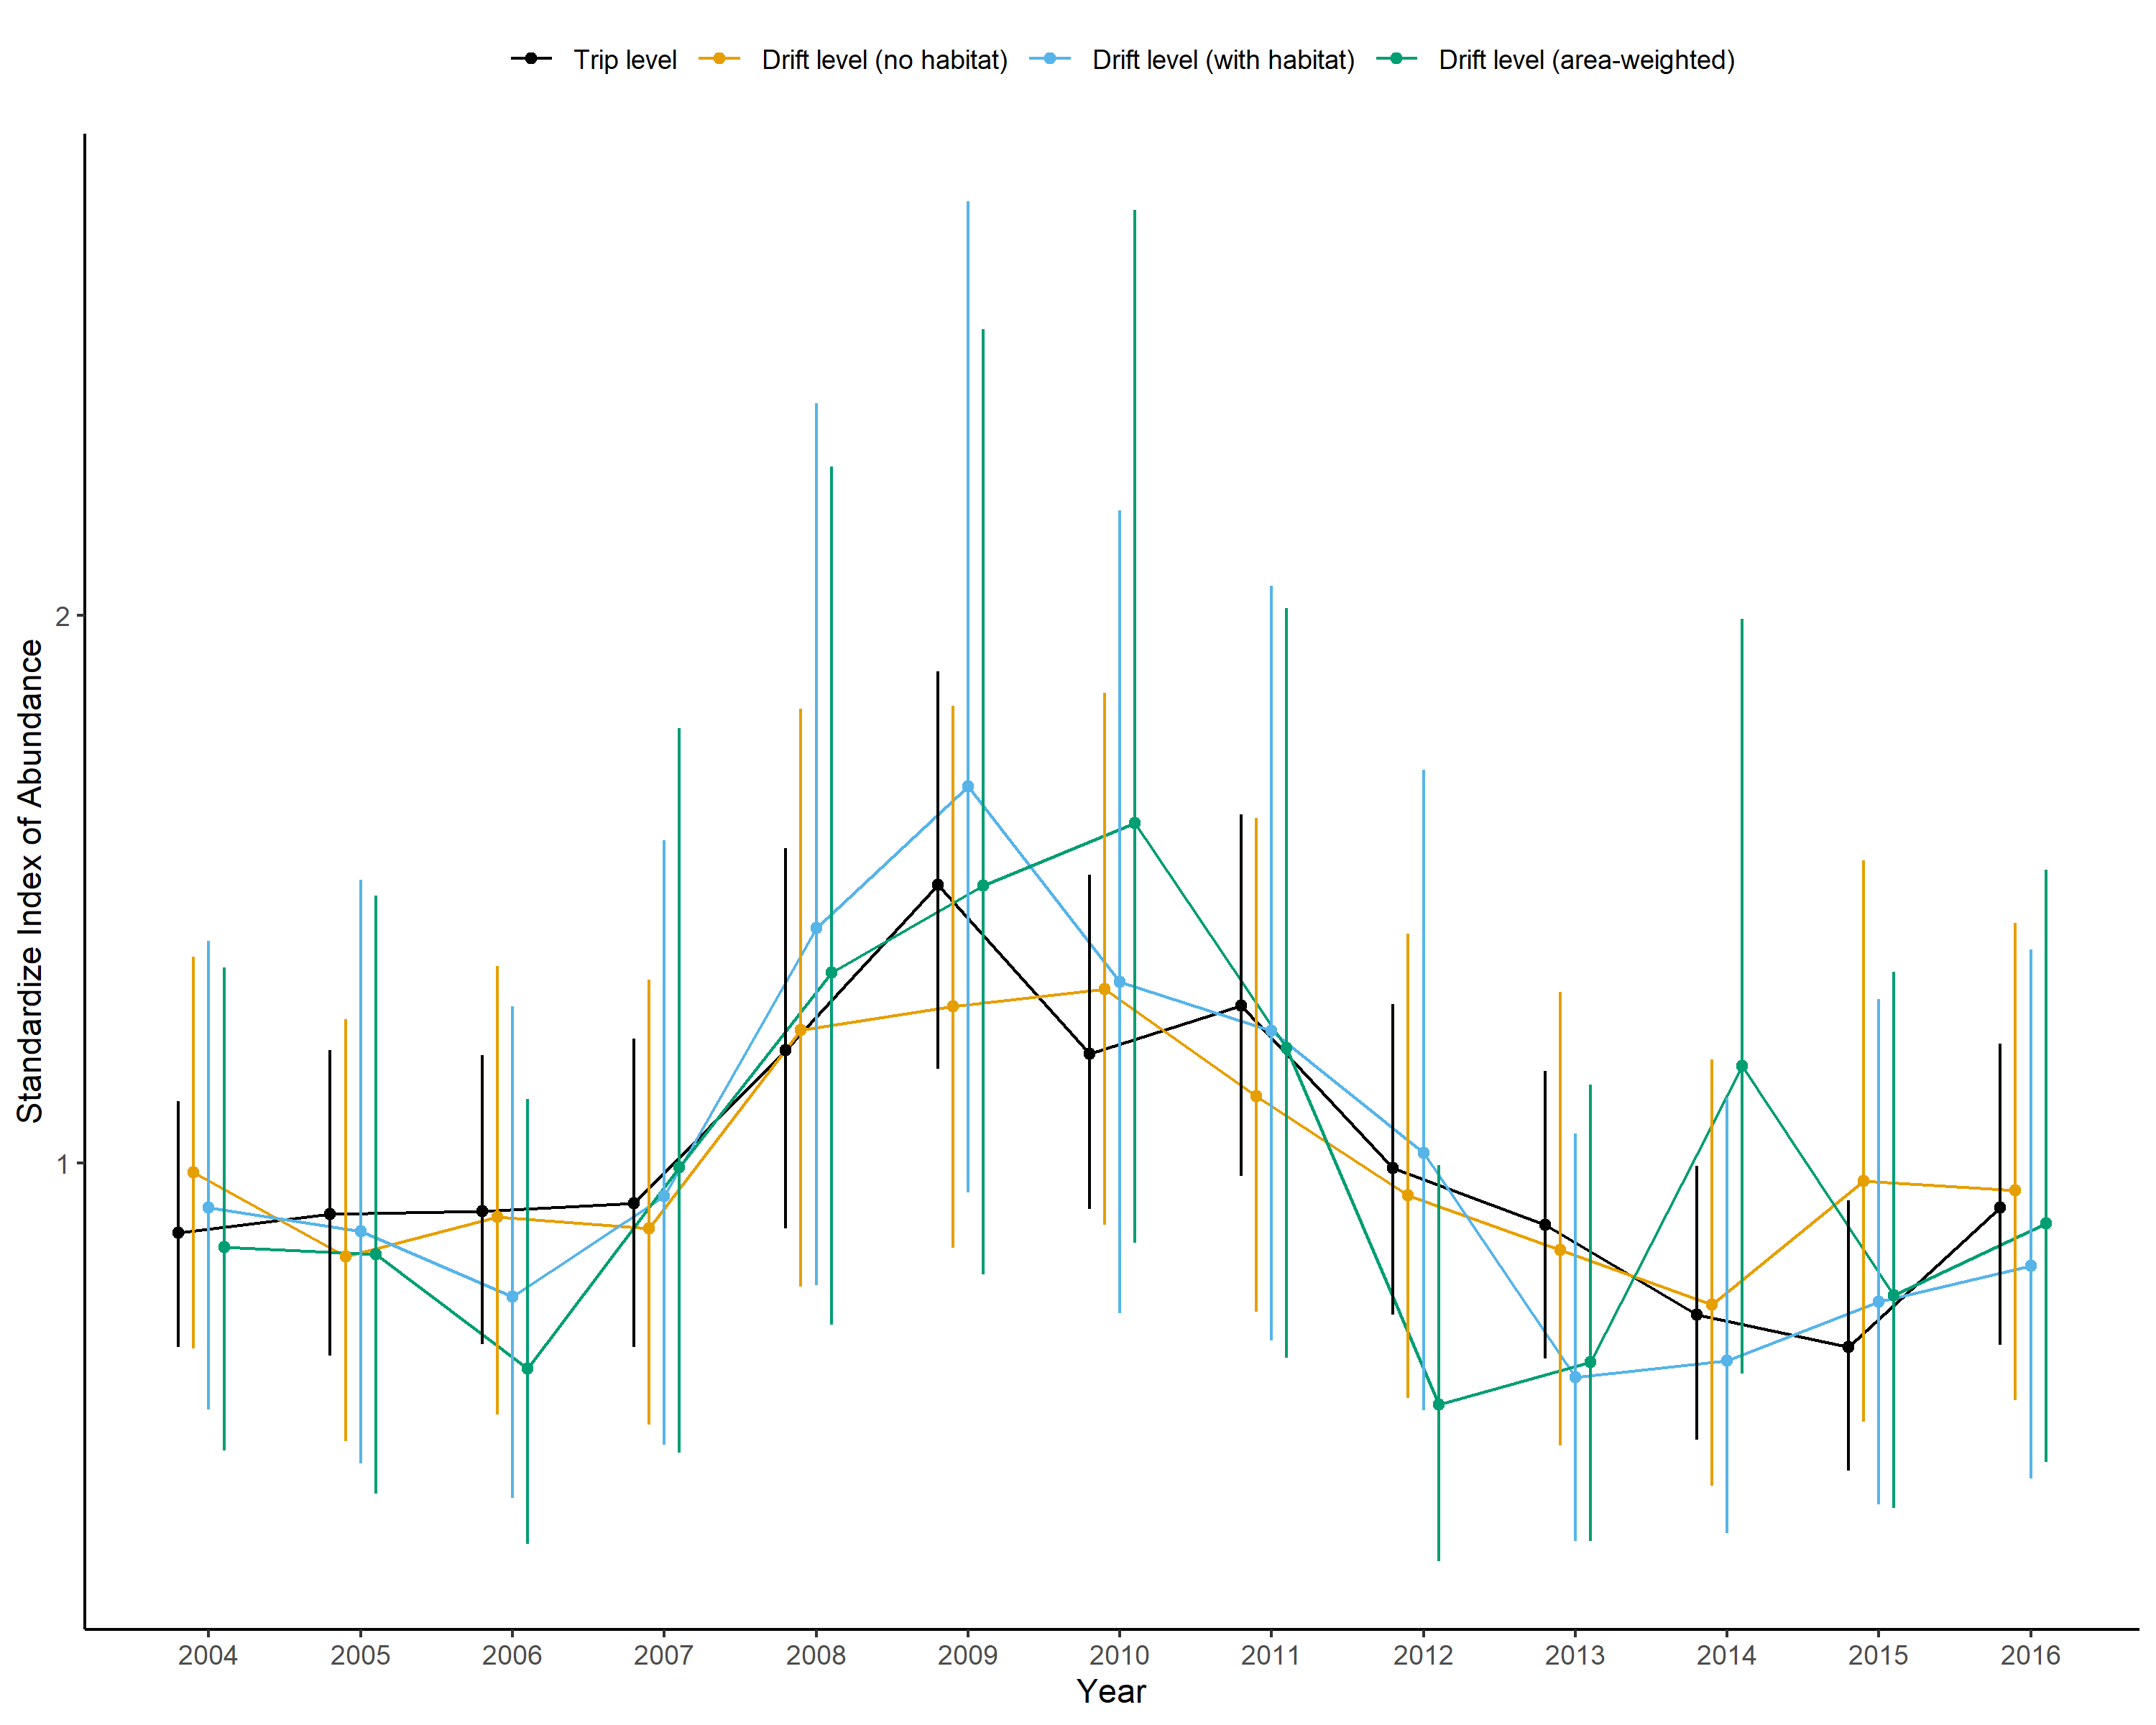
\includegraphics[width=3in,height=\textheight]{figures/china_indices.png}

}

\caption{\label{fig-china-indices}China rockfish}

}

\end{minipage}%
\newline
\begin{minipage}[t]{0.50\linewidth}

{\centering 

\raisebox{-\height}{

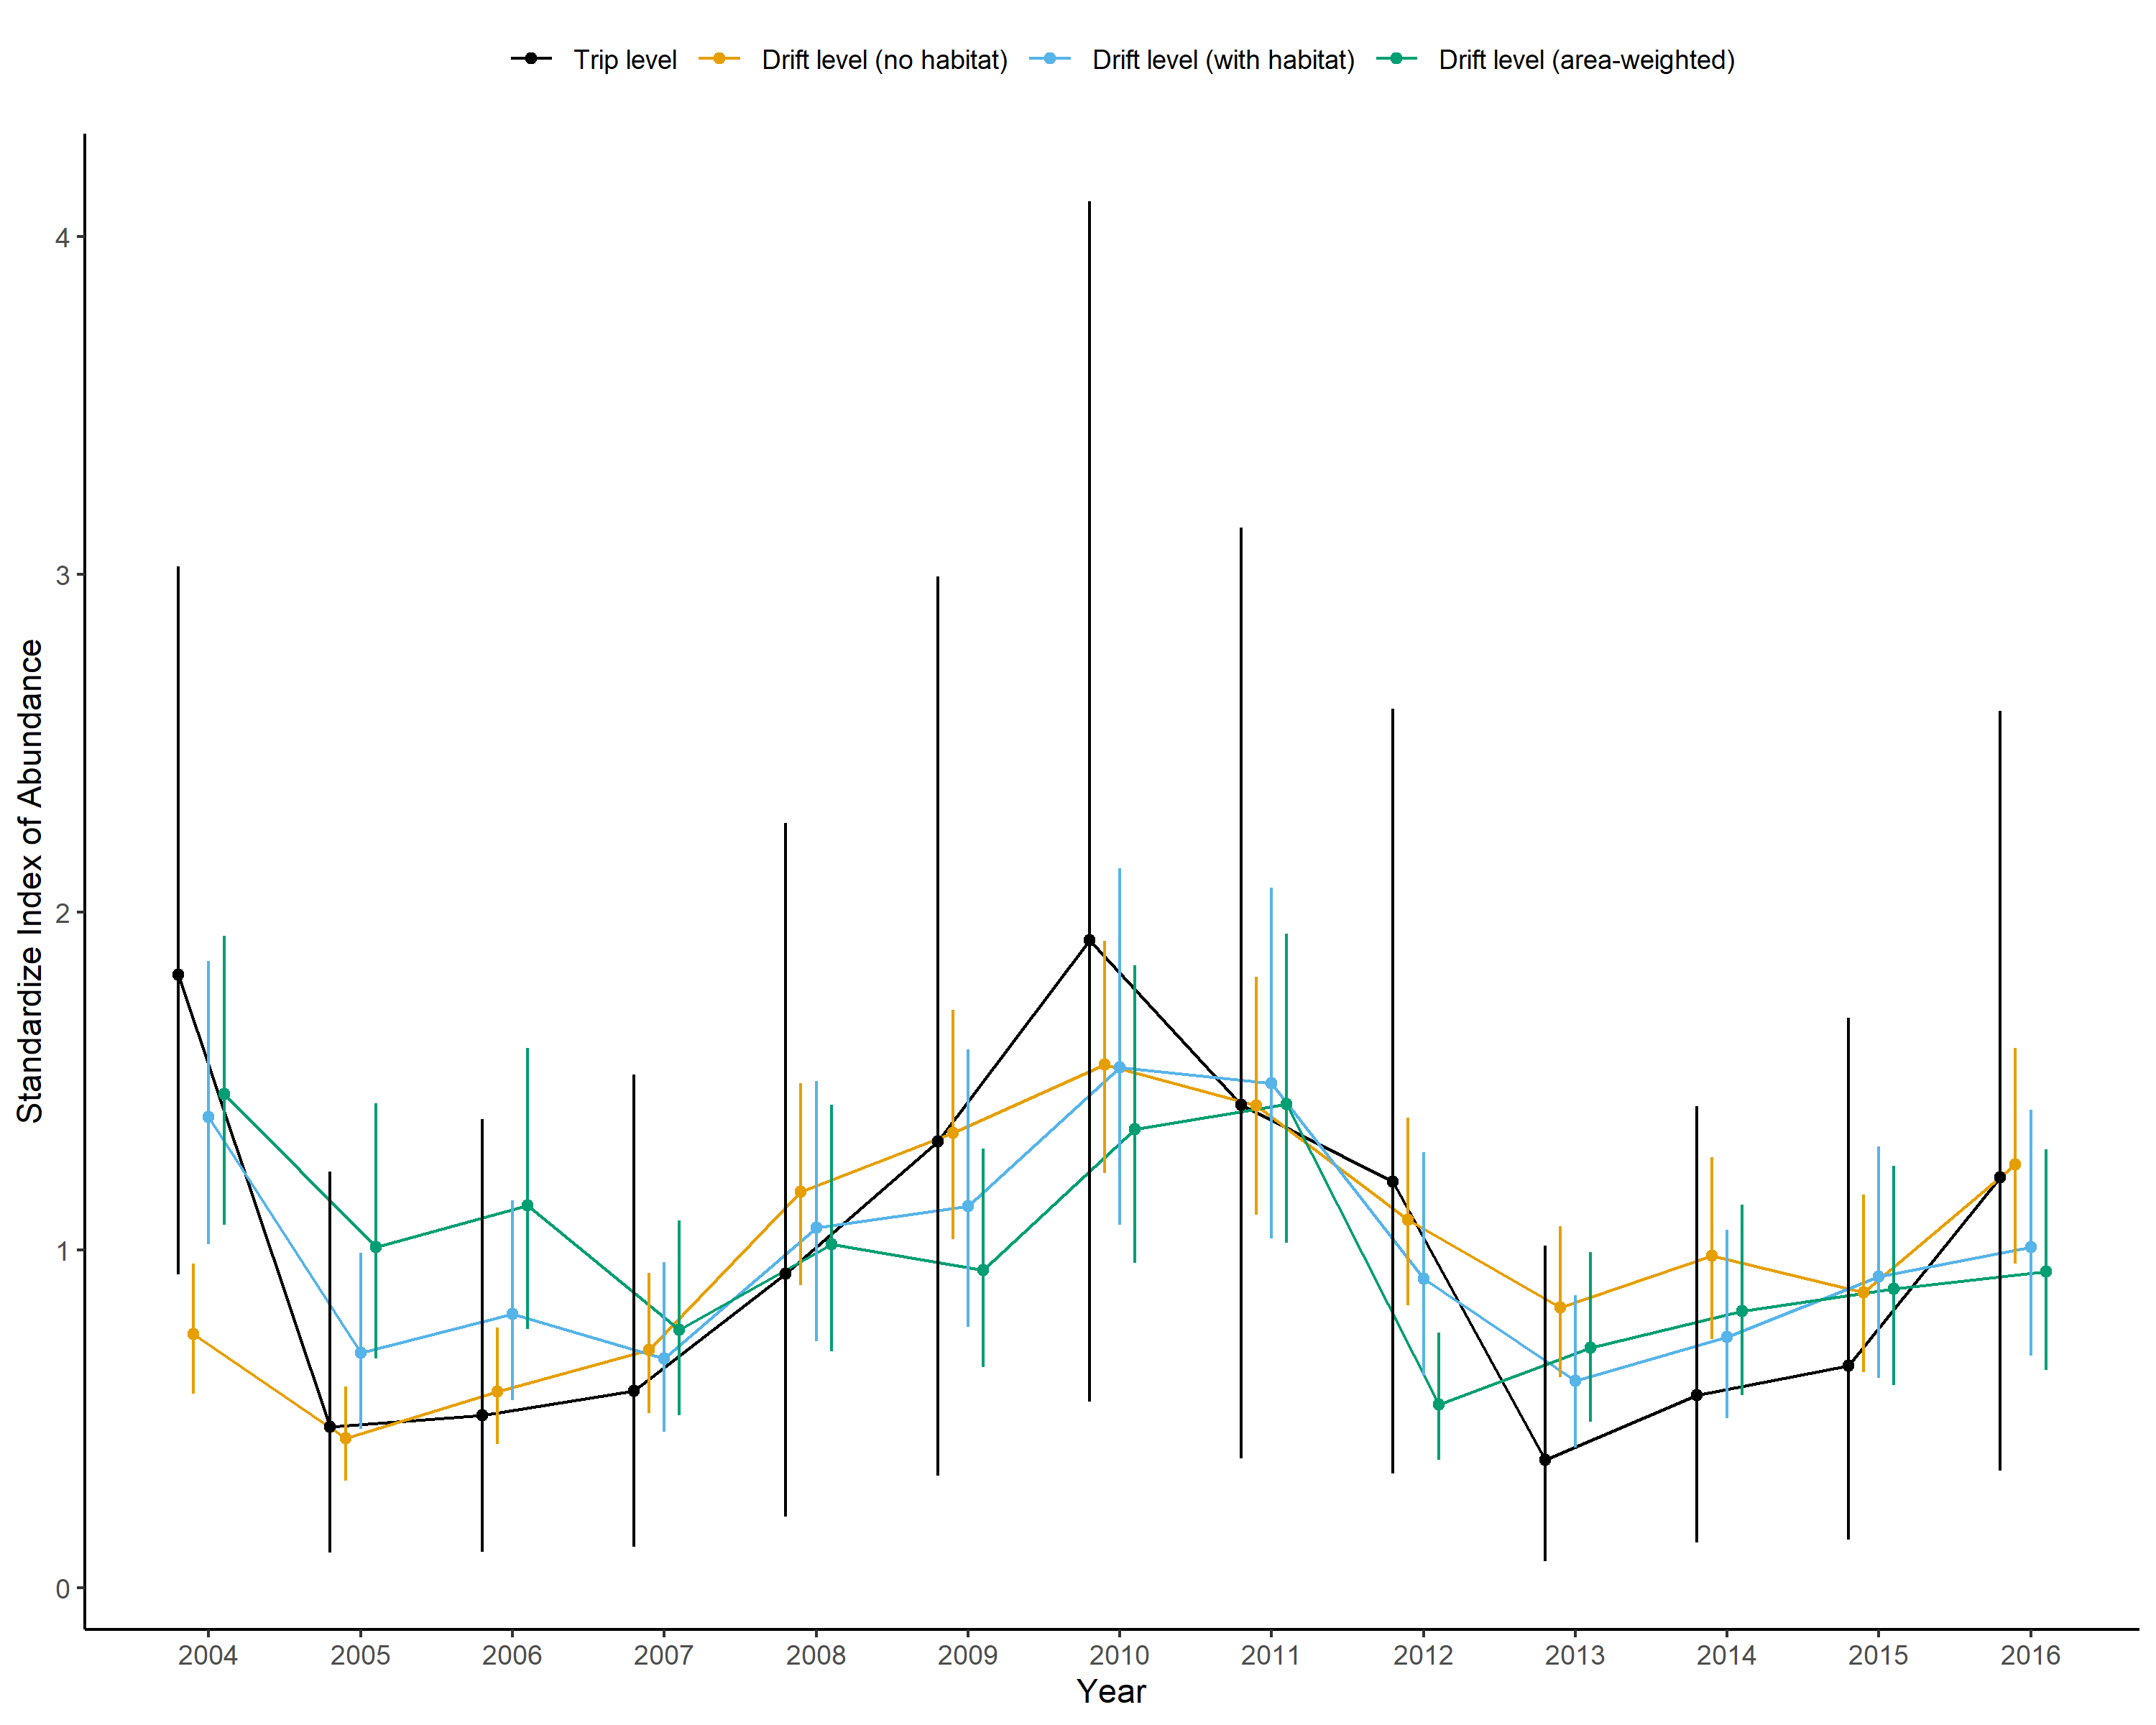
\includegraphics[width=3in,height=\textheight]{figures/gopher_indices.png}

}

\caption{\label{fig-gopher-indices}Gopher rockfish}

}

\end{minipage}%
%
\begin{minipage}[t]{0.50\linewidth}

{\centering 

\raisebox{-\height}{

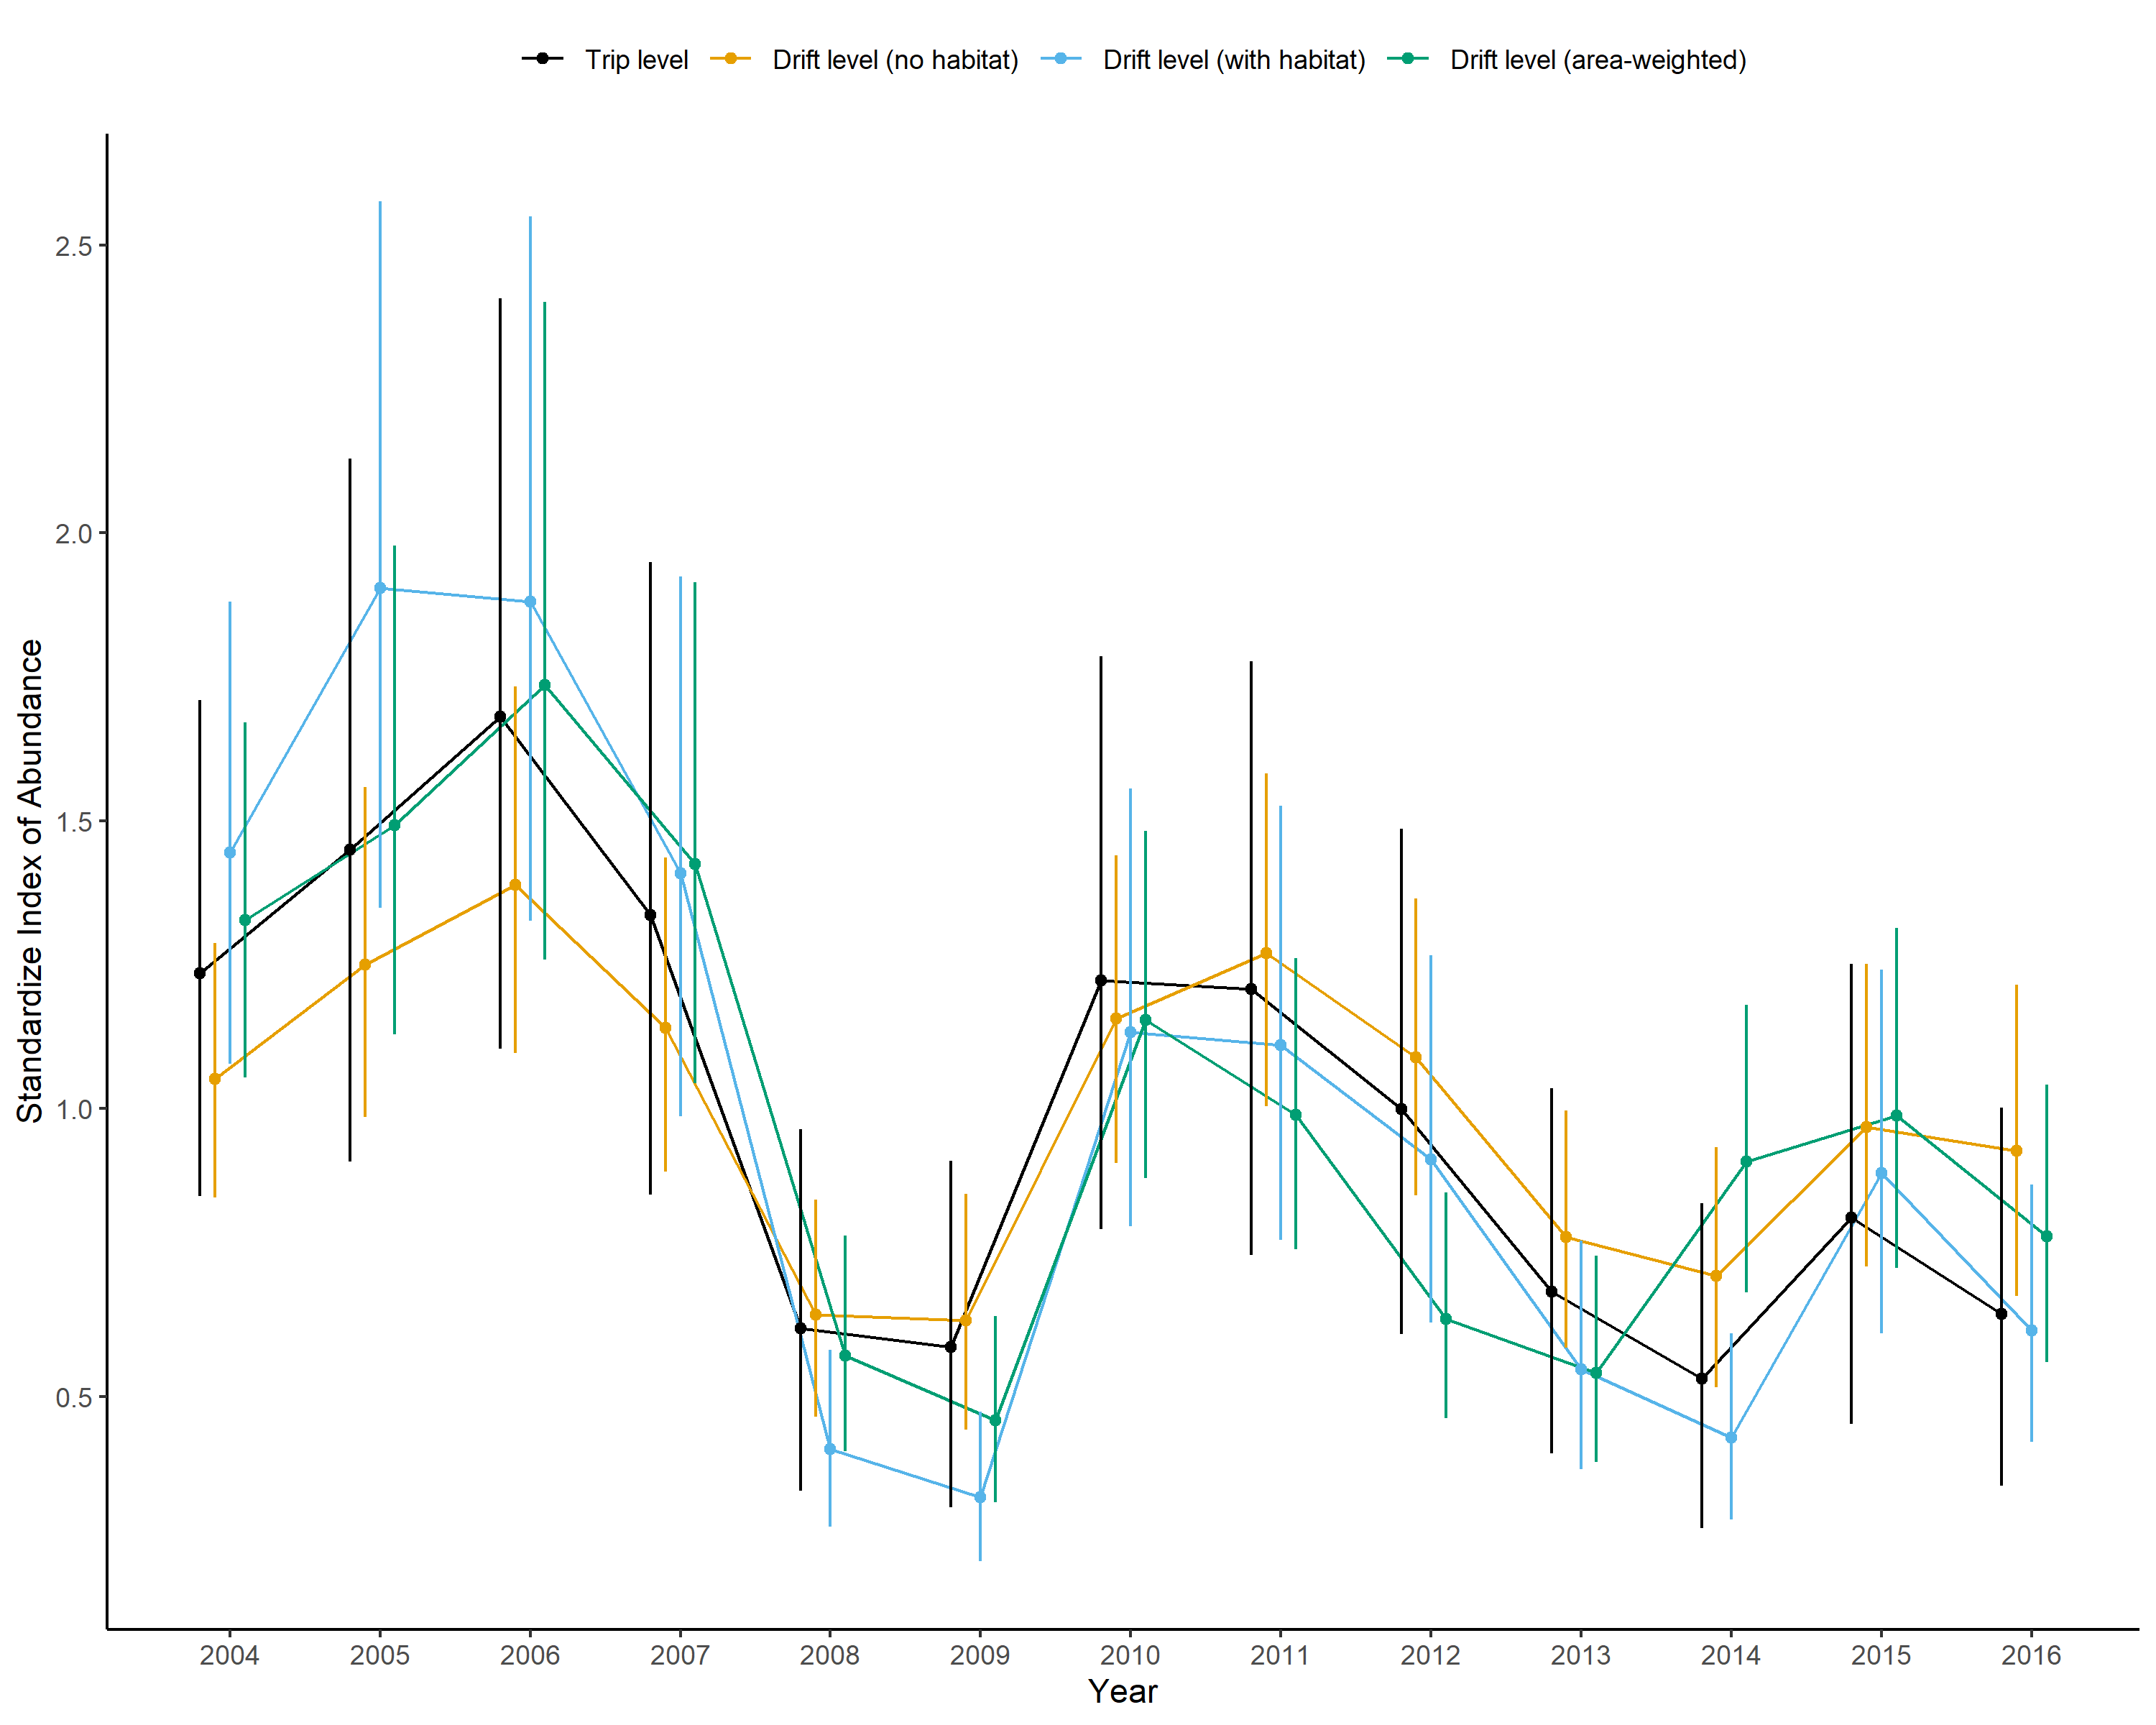
\includegraphics[width=3in,height=\textheight]{figures/vermilion_indices.png}

}

\caption{\label{fig-vermilion-indices}Vermilion rockfish}

}

\end{minipage}%
\newline
\begin{minipage}[t]{0.50\linewidth}

{\centering 

Scaled indices of abundance for four data filtering methods explored.

}

\end{minipage}%

\end{figure}

\FloatBarrier

\#Supplemental tables and figures

\begin{figure}

\begin{minipage}[t]{0.50\linewidth}

{\centering 

\raisebox{-\height}{

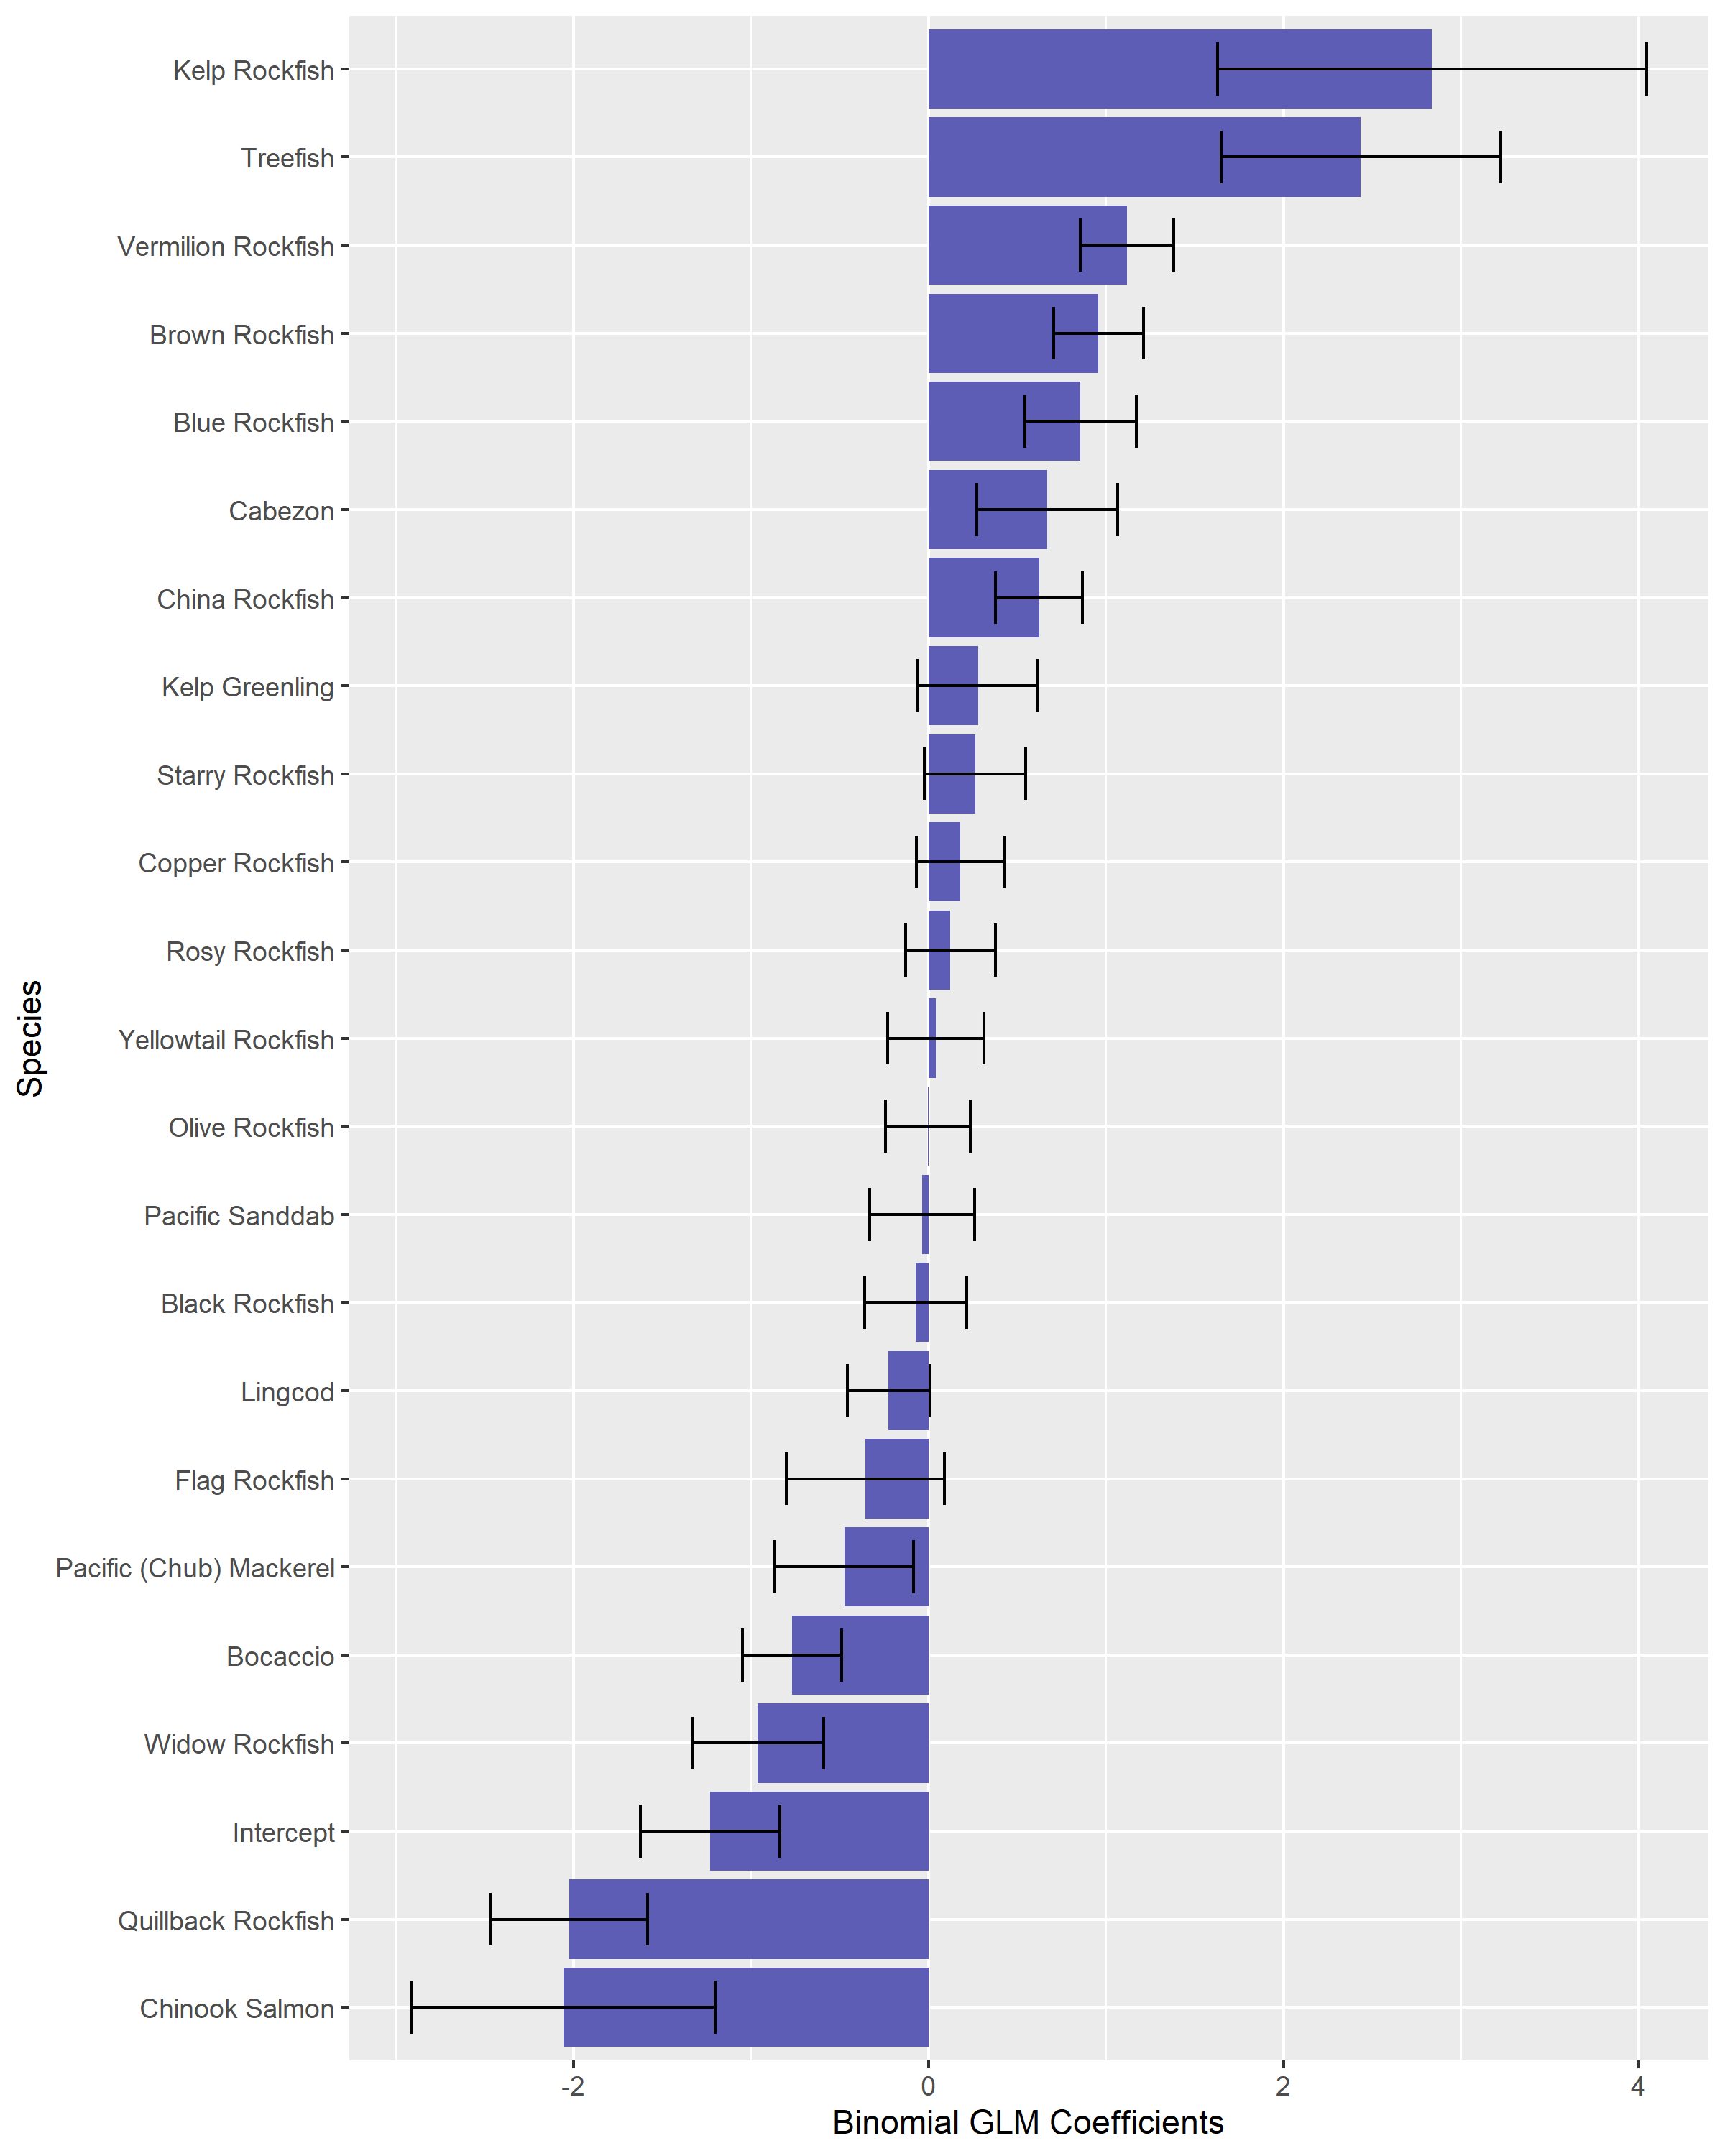
\includegraphics[width=2.75in,height=\textheight]{figures/gopher_trip_sm.png}

}

}

\subcaption{\label{fig-gopher-trips}Gopher rockfish trip level}
\end{minipage}%
%
\begin{minipage}[t]{0.50\linewidth}

{\centering 

\raisebox{-\height}{

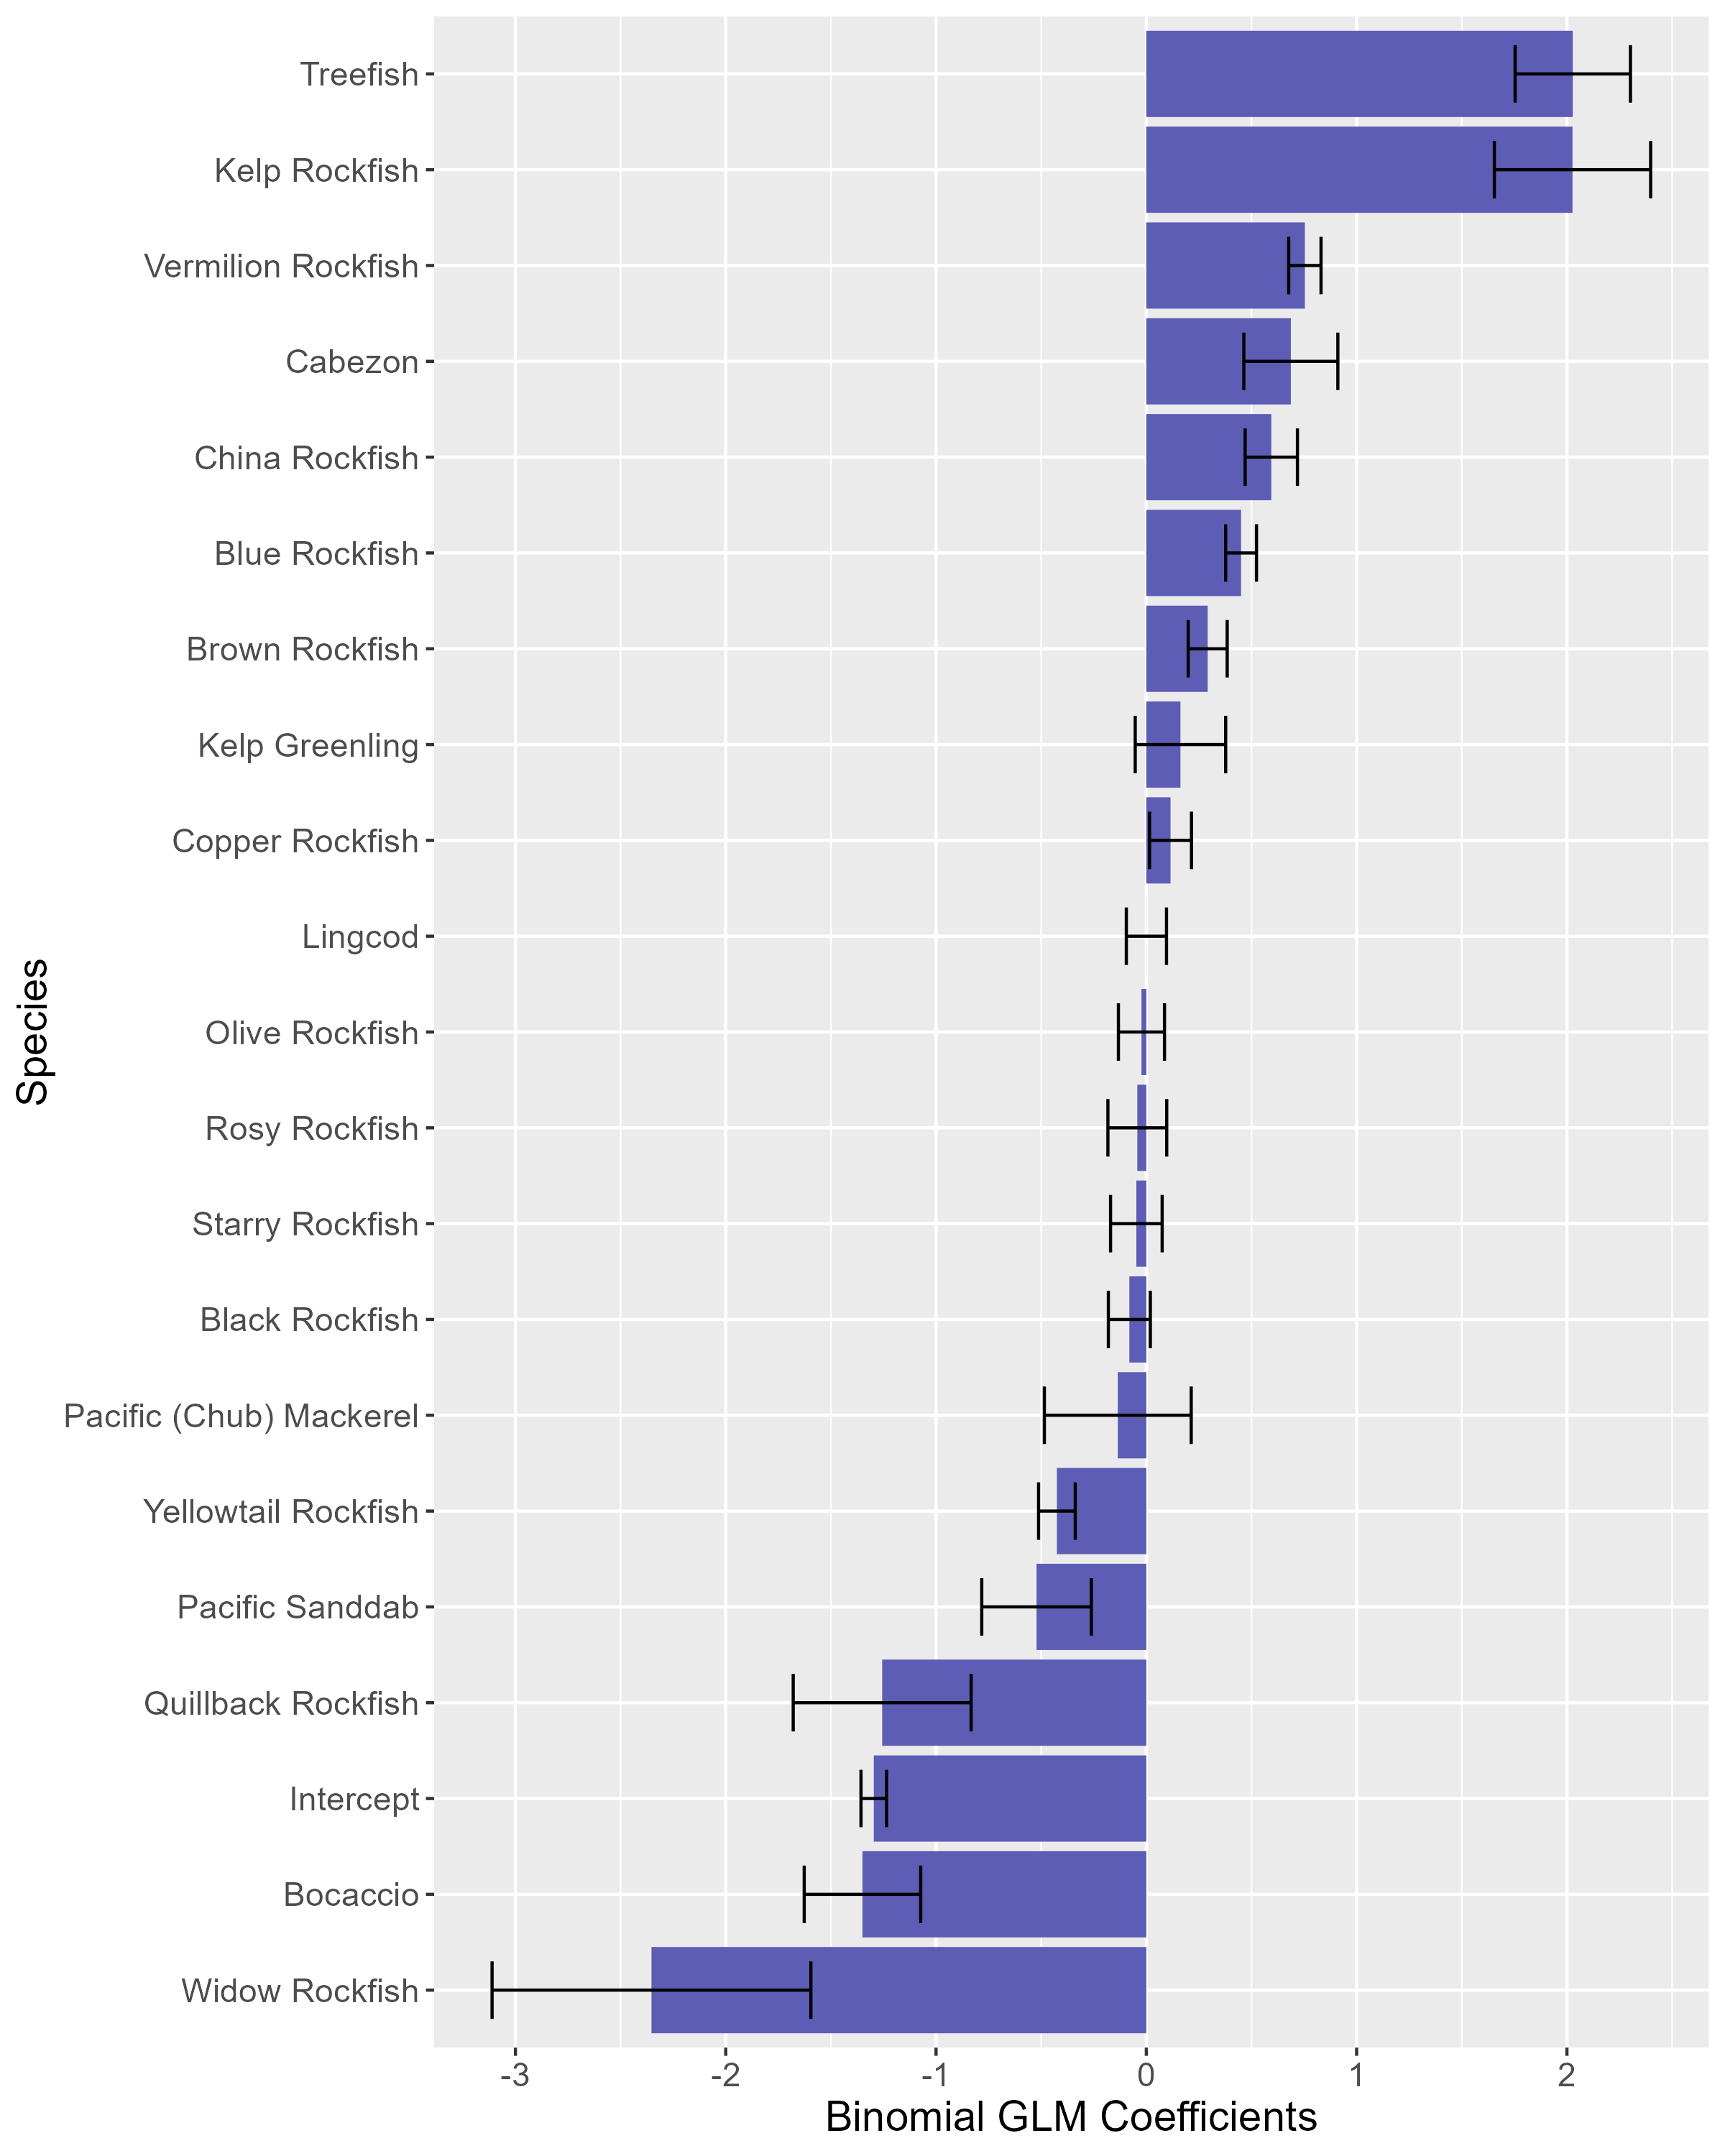
\includegraphics[width=2.75in,height=\textheight]{figures/gopher_drift_sm.png}

}

}

\subcaption{\label{fig-gopher-drifts}Gopher rockfish drift level}
\end{minipage}%
\newline
\begin{minipage}[t]{0.50\linewidth}

{\centering 

\raisebox{-\height}{

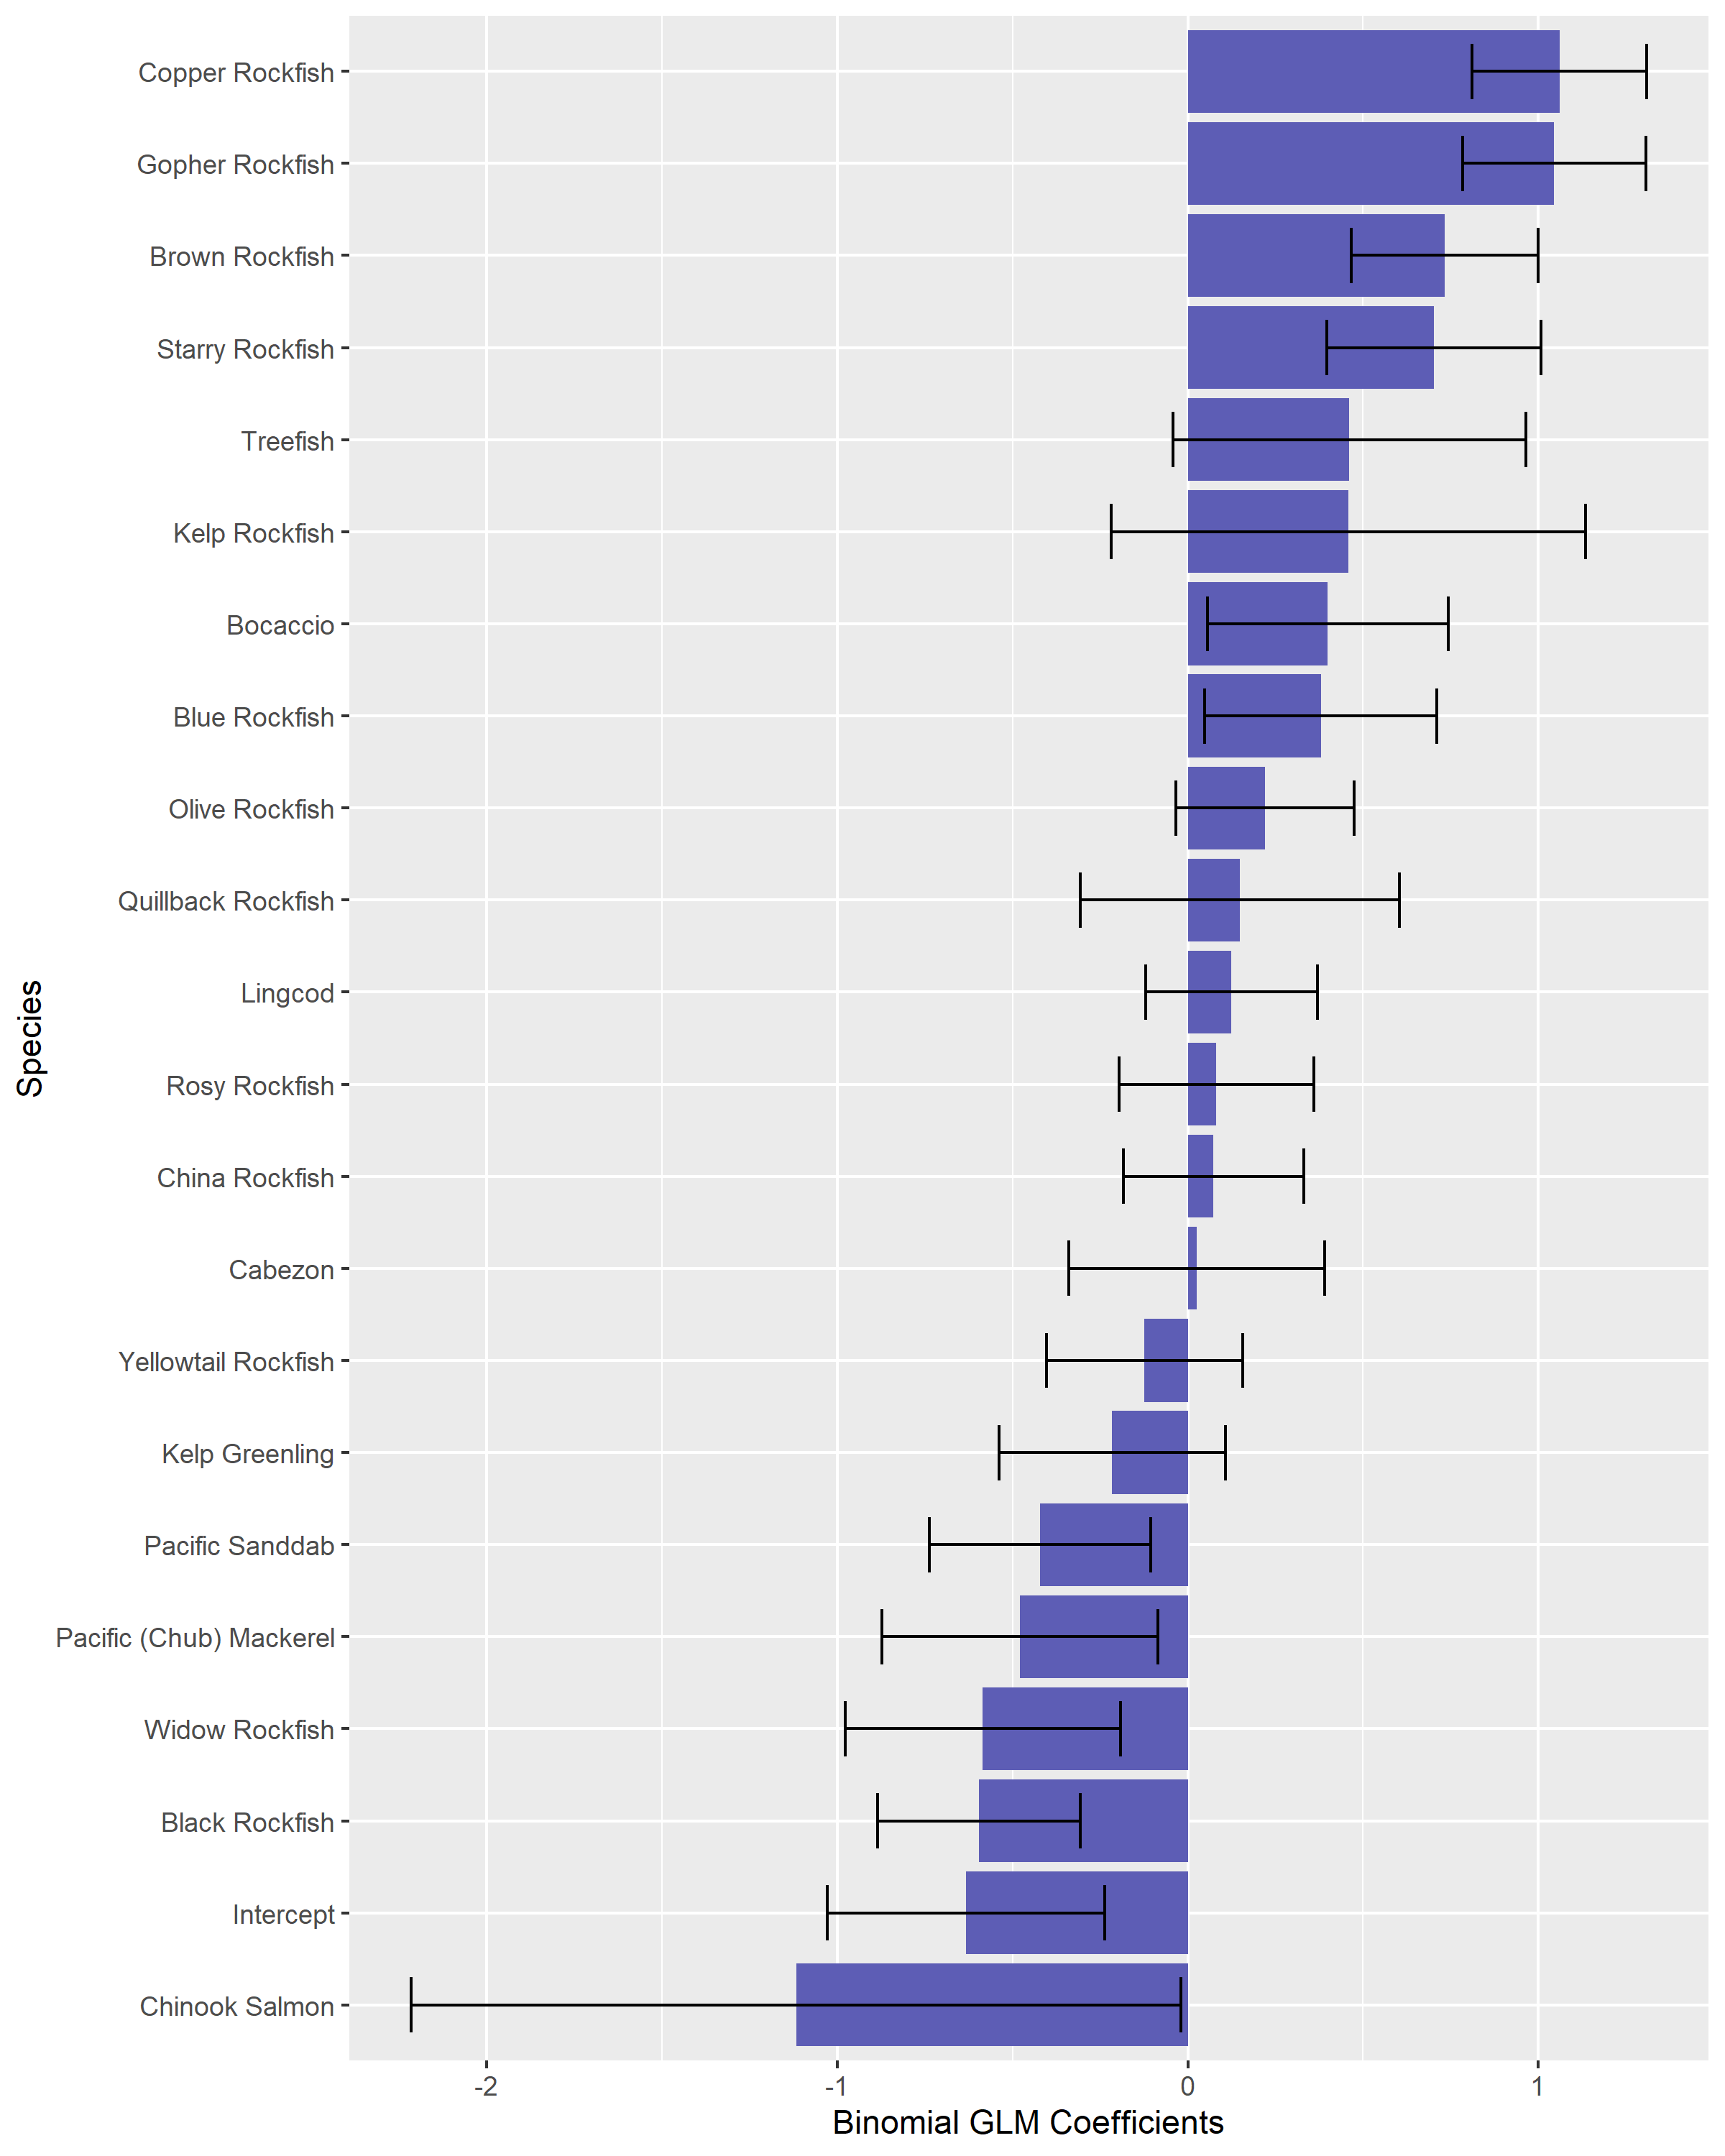
\includegraphics[width=2.75in,height=\textheight]{figures/vermilion_trip_sm.png}

}

}

\subcaption{\label{fig-vermilion-trips}Vermilion rockfish trip level}
\end{minipage}%
%
\begin{minipage}[t]{0.50\linewidth}

{\centering 

\raisebox{-\height}{

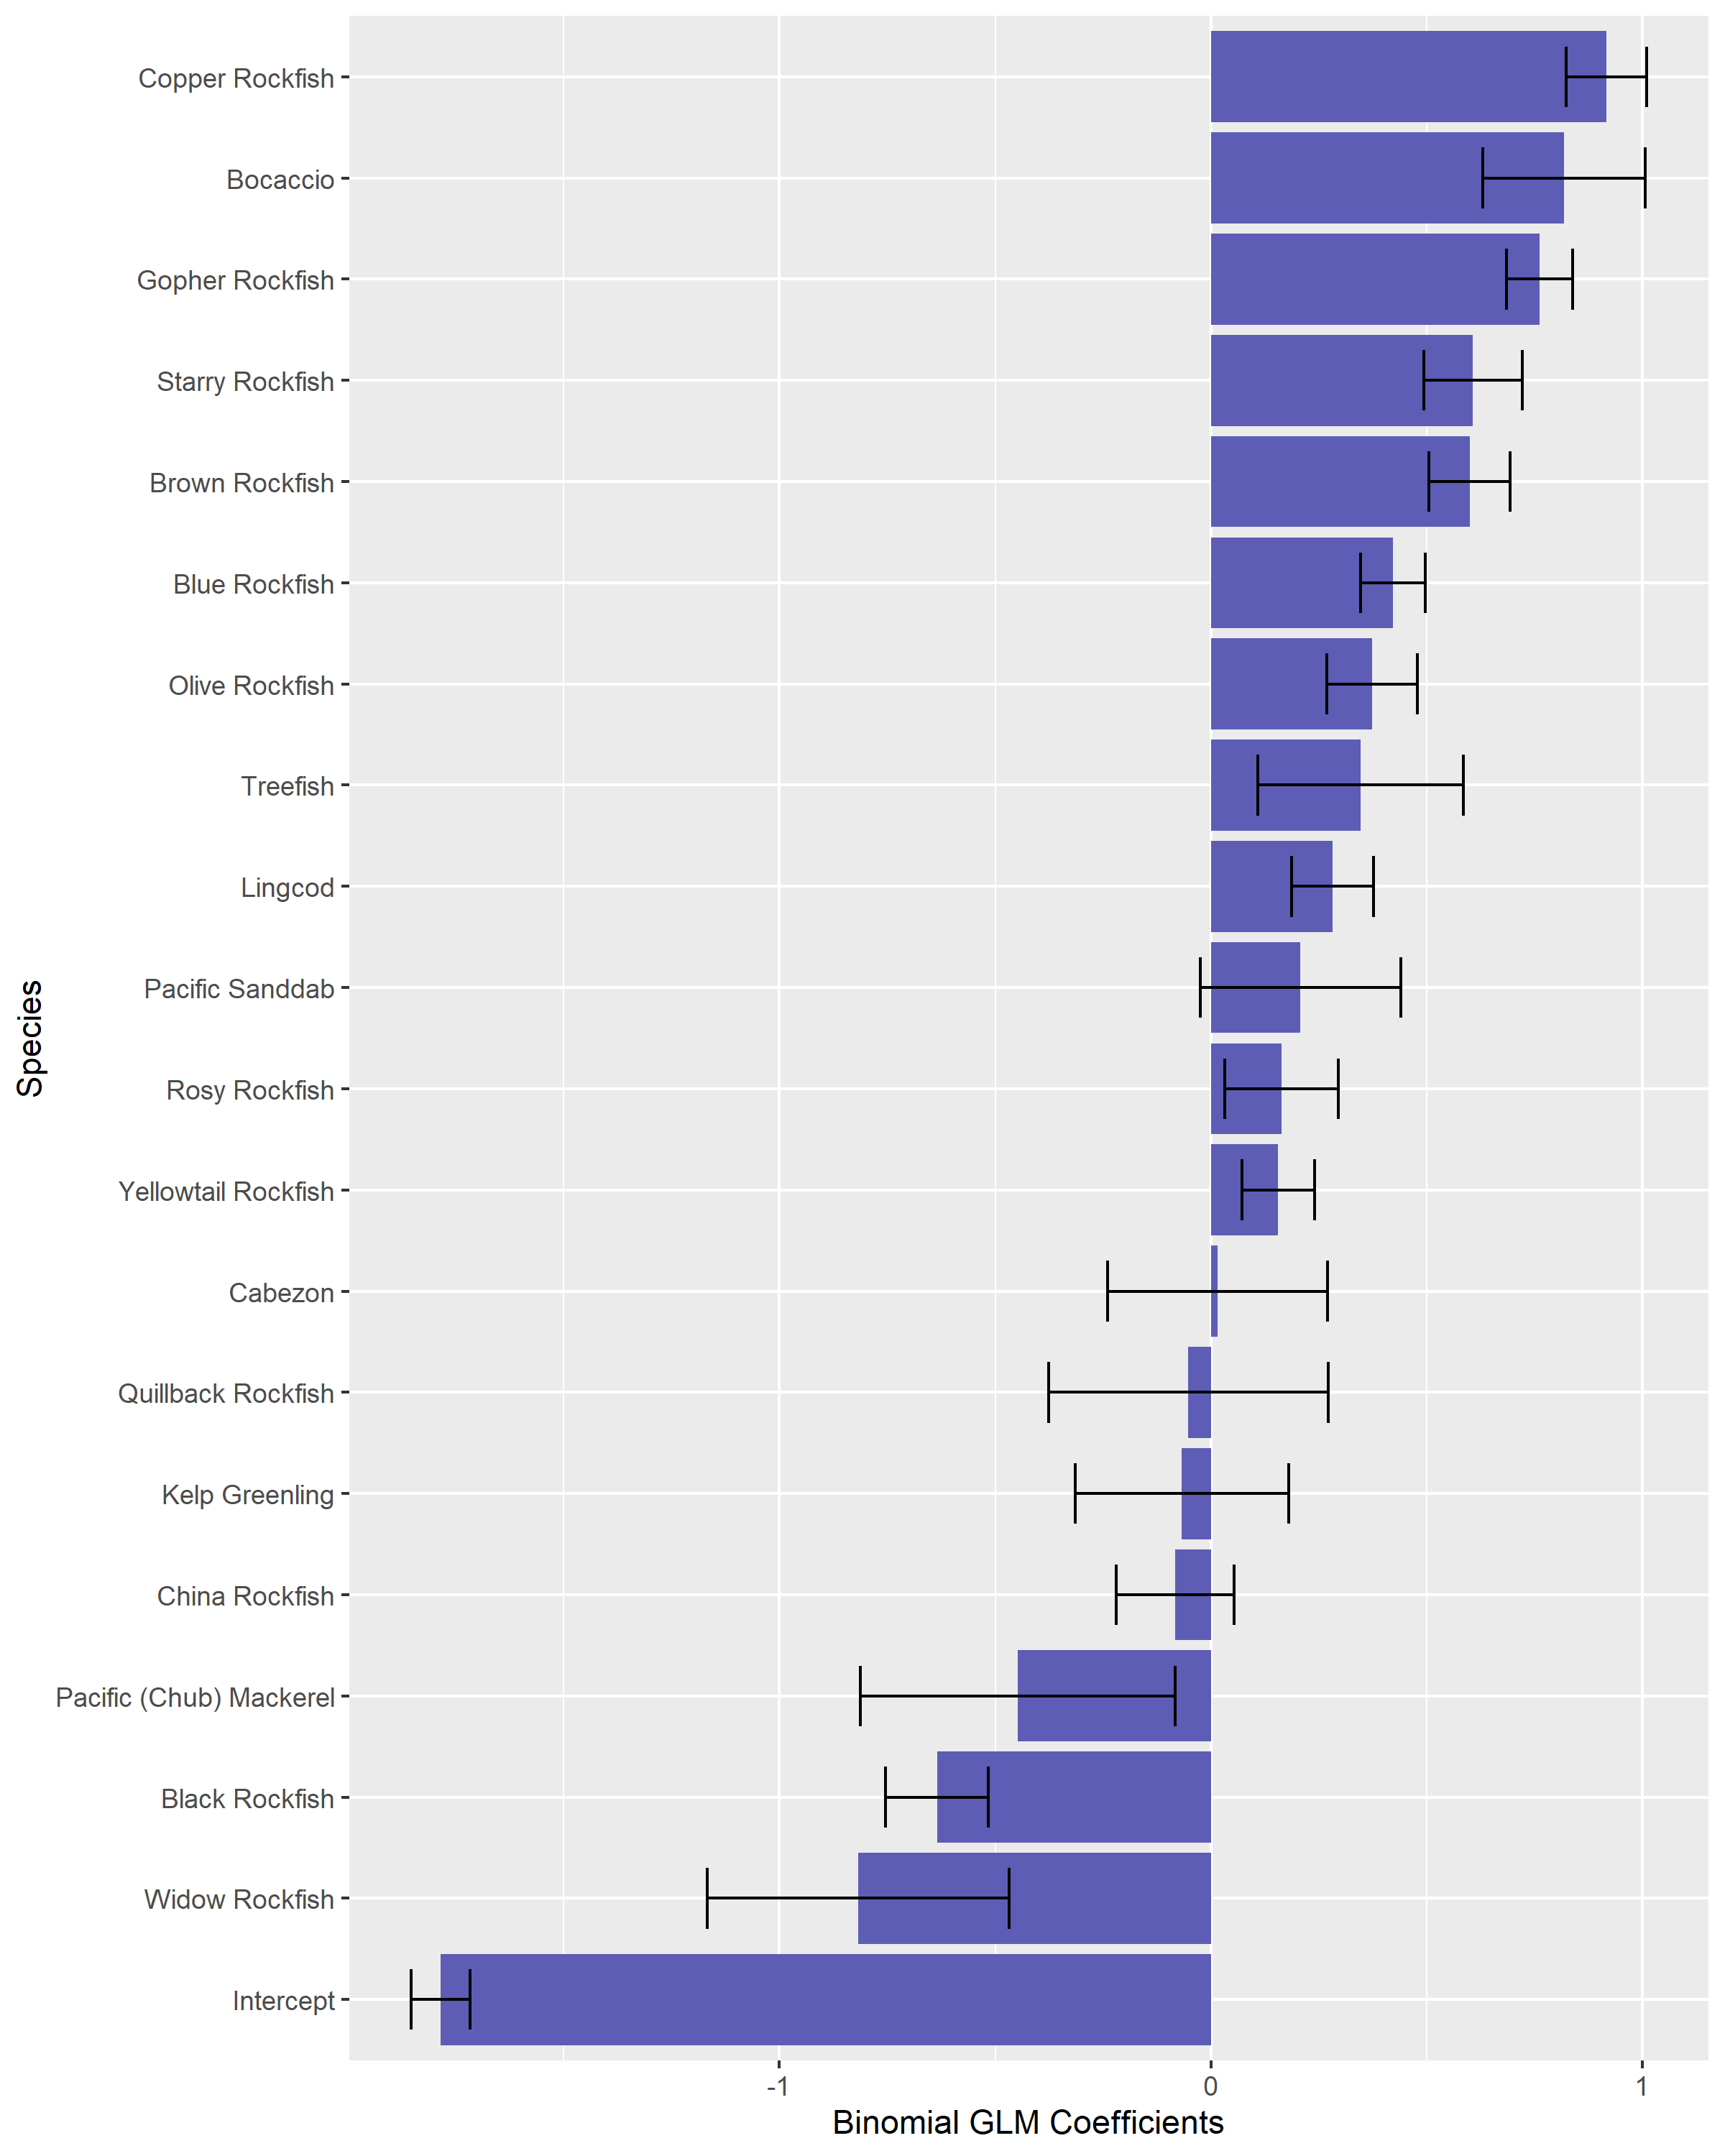
\includegraphics[width=2.75in,height=\textheight]{figures/vermilion_drift_sm.png}

}

}

\subcaption{\label{fig-vermilion-drifts}Vermilion rockfish driftlevel}
\end{minipage}%

\caption{\label{fig-sm3}The species coefficients from the
Stephens-MacCall method at the trip-level and drift-level for species
not presented in the main body of the paper.}

\end{figure}

\begin{figure}

\begin{minipage}[t]{0.50\linewidth}

{\centering 

\raisebox{-\height}{

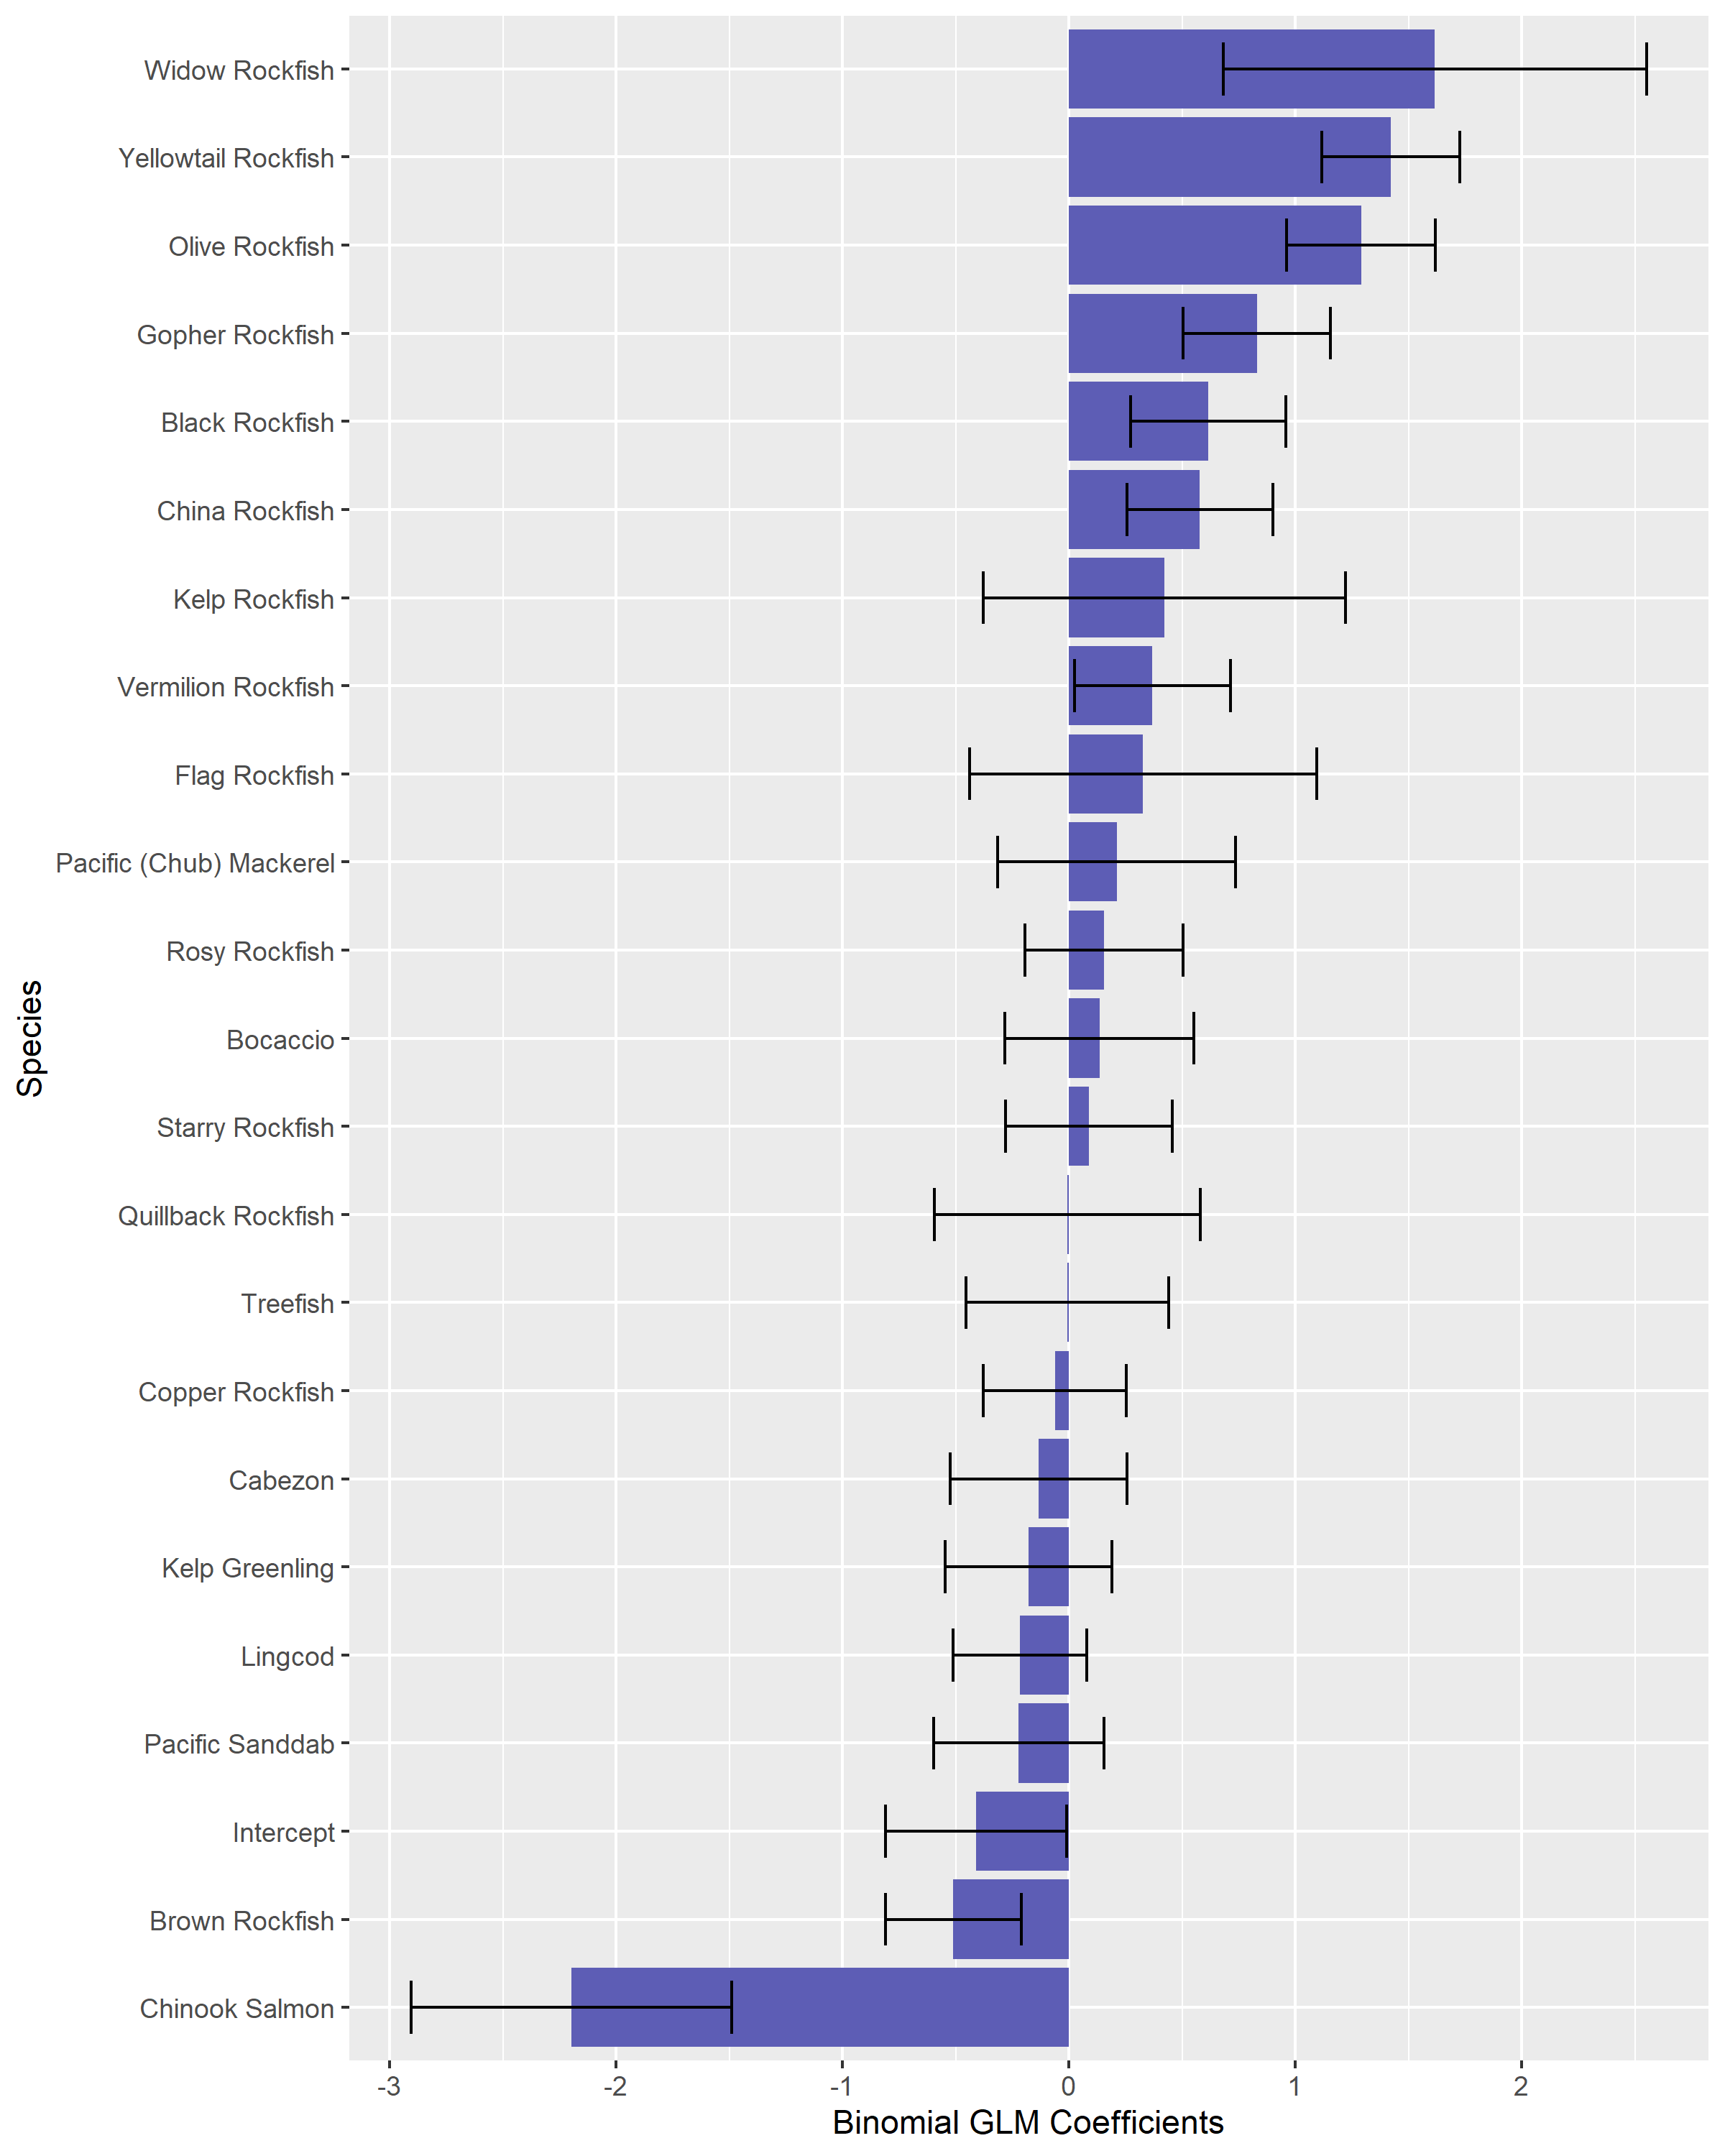
\includegraphics[width=2.75in,height=\textheight]{figures/blue_trip_sm.png}

}

\caption{\label{fig-blue-tripsm}Blue rockfish trip level}

}

\end{minipage}%
%
\begin{minipage}[t]{0.50\linewidth}

{\centering 

\raisebox{-\height}{

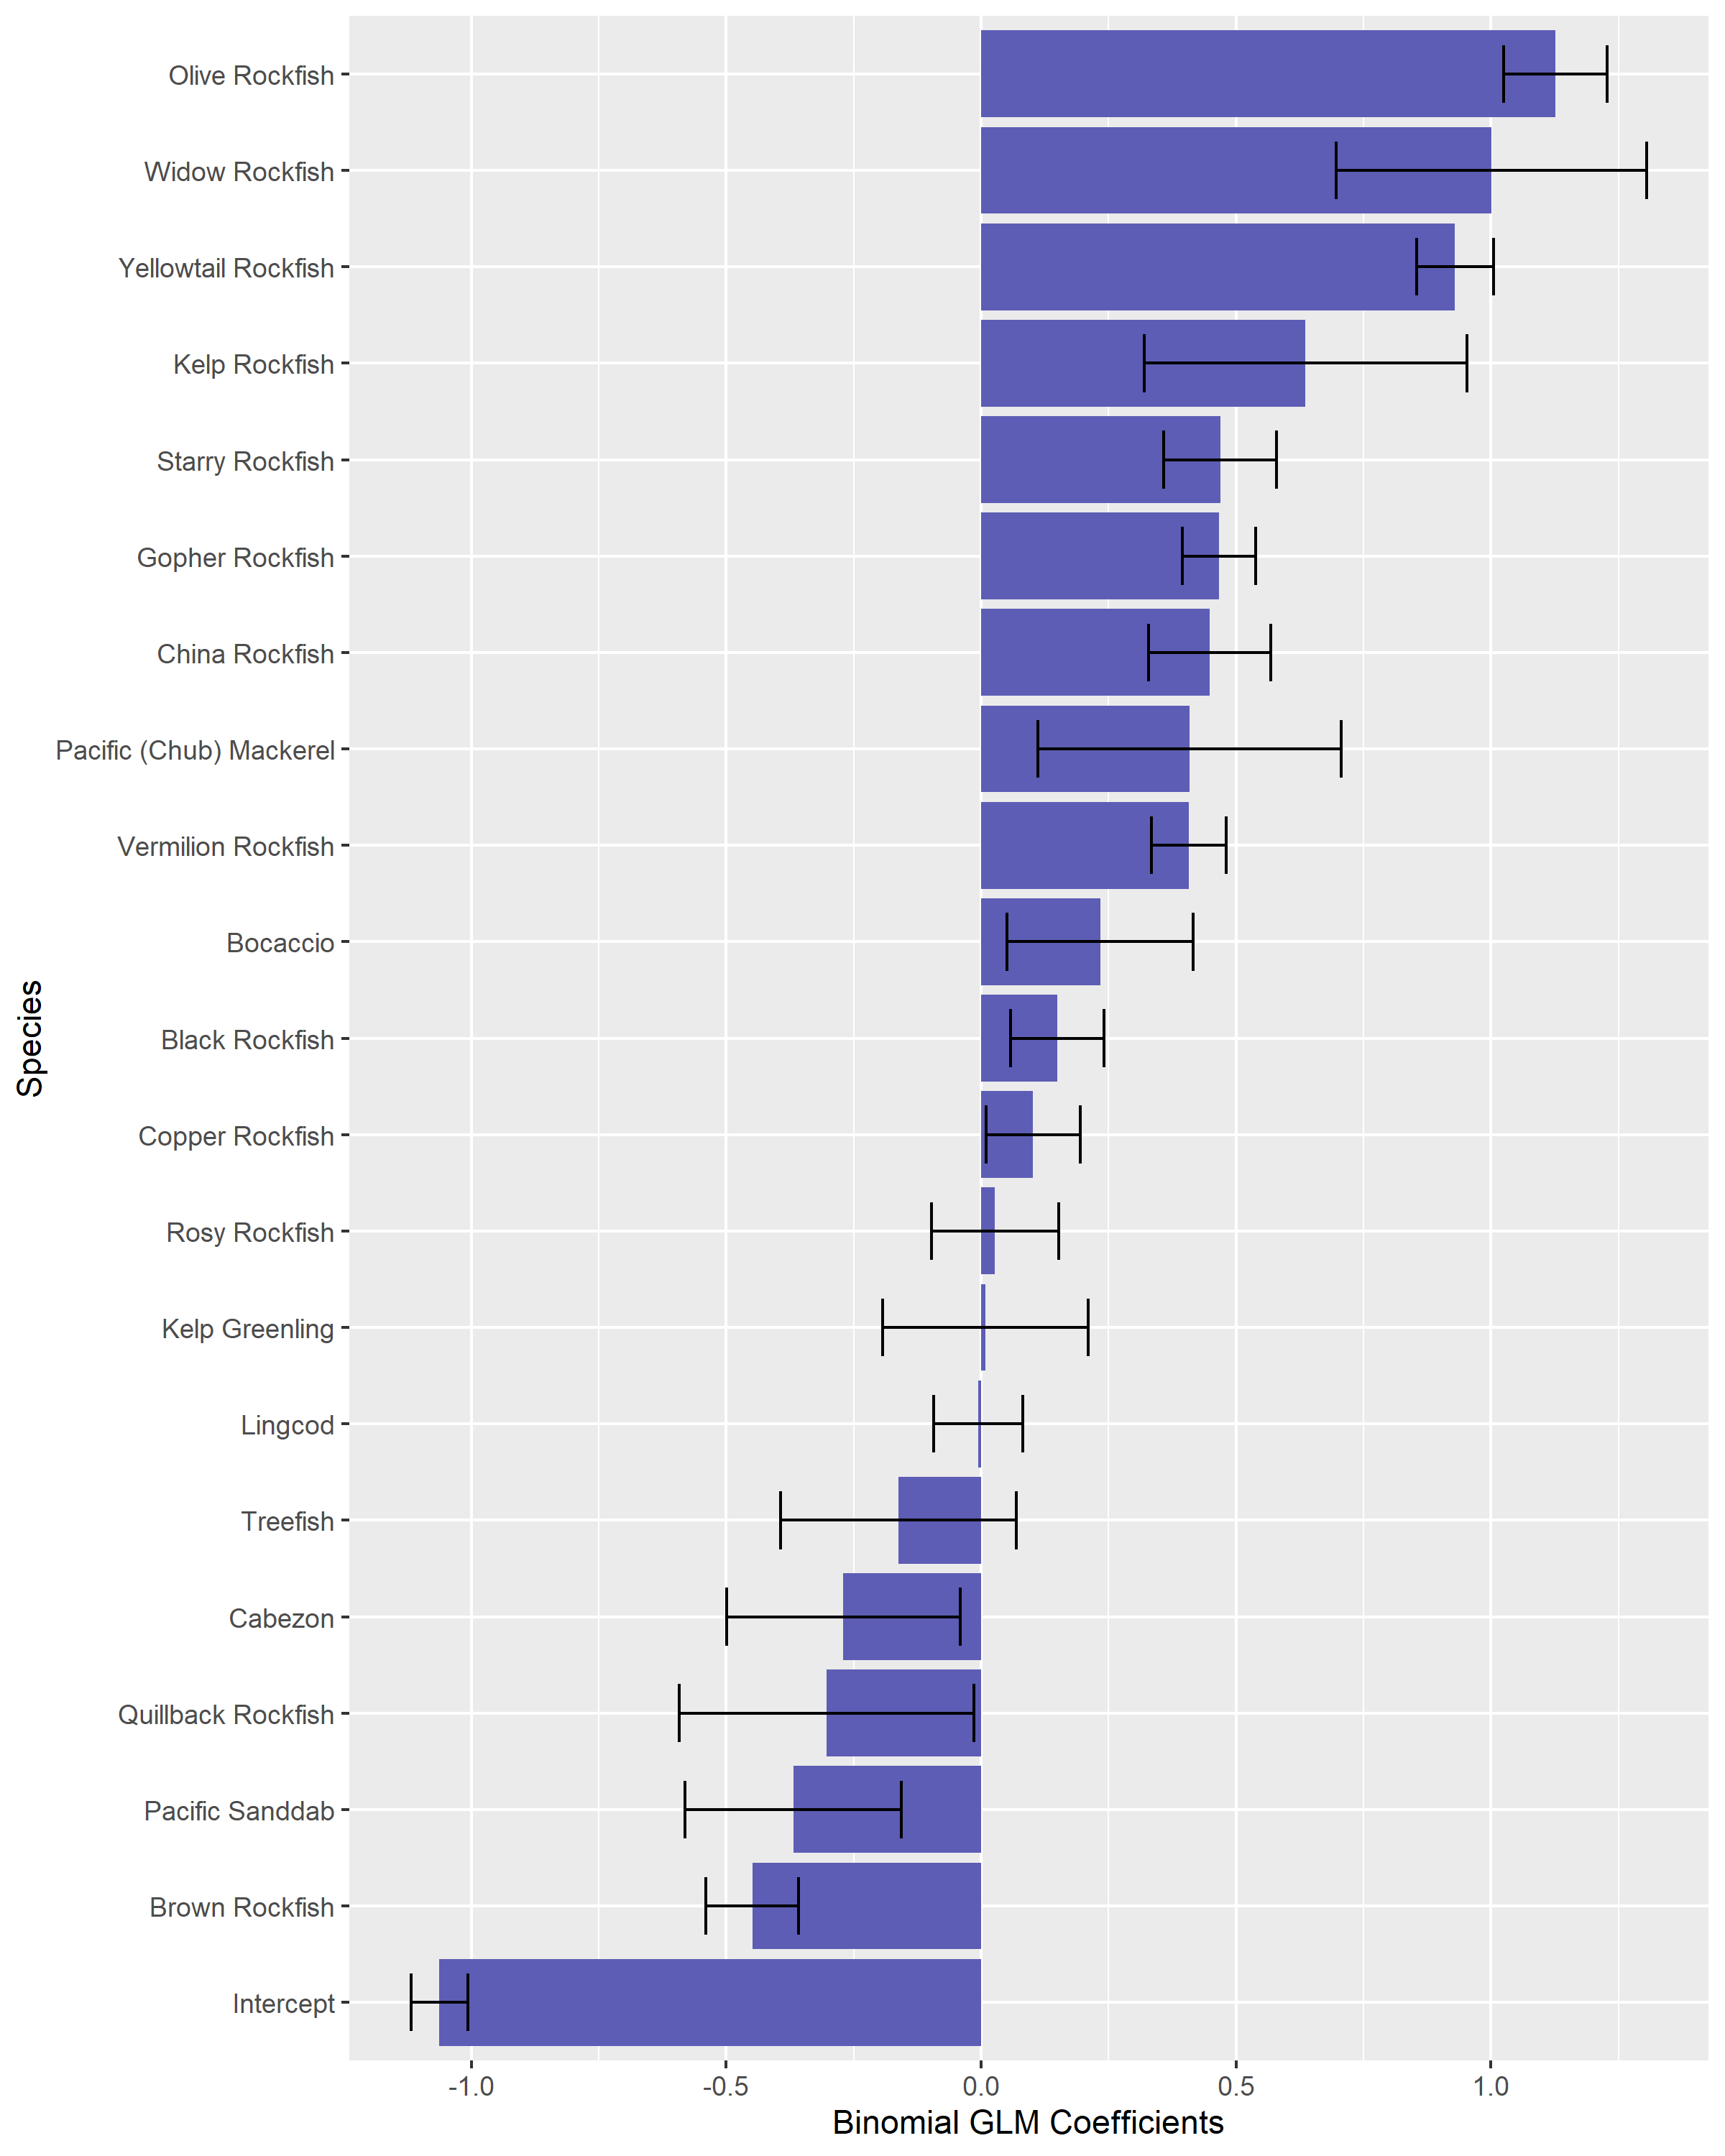
\includegraphics[width=2.75in,height=\textheight]{figures/blue_drift_sm.png}

}

\caption{\label{fig-blue-driftsm}Blue rockfish drift level}

}

\end{minipage}%
\newline
\begin{minipage}[t]{0.50\linewidth}

{\centering 

\raisebox{-\height}{

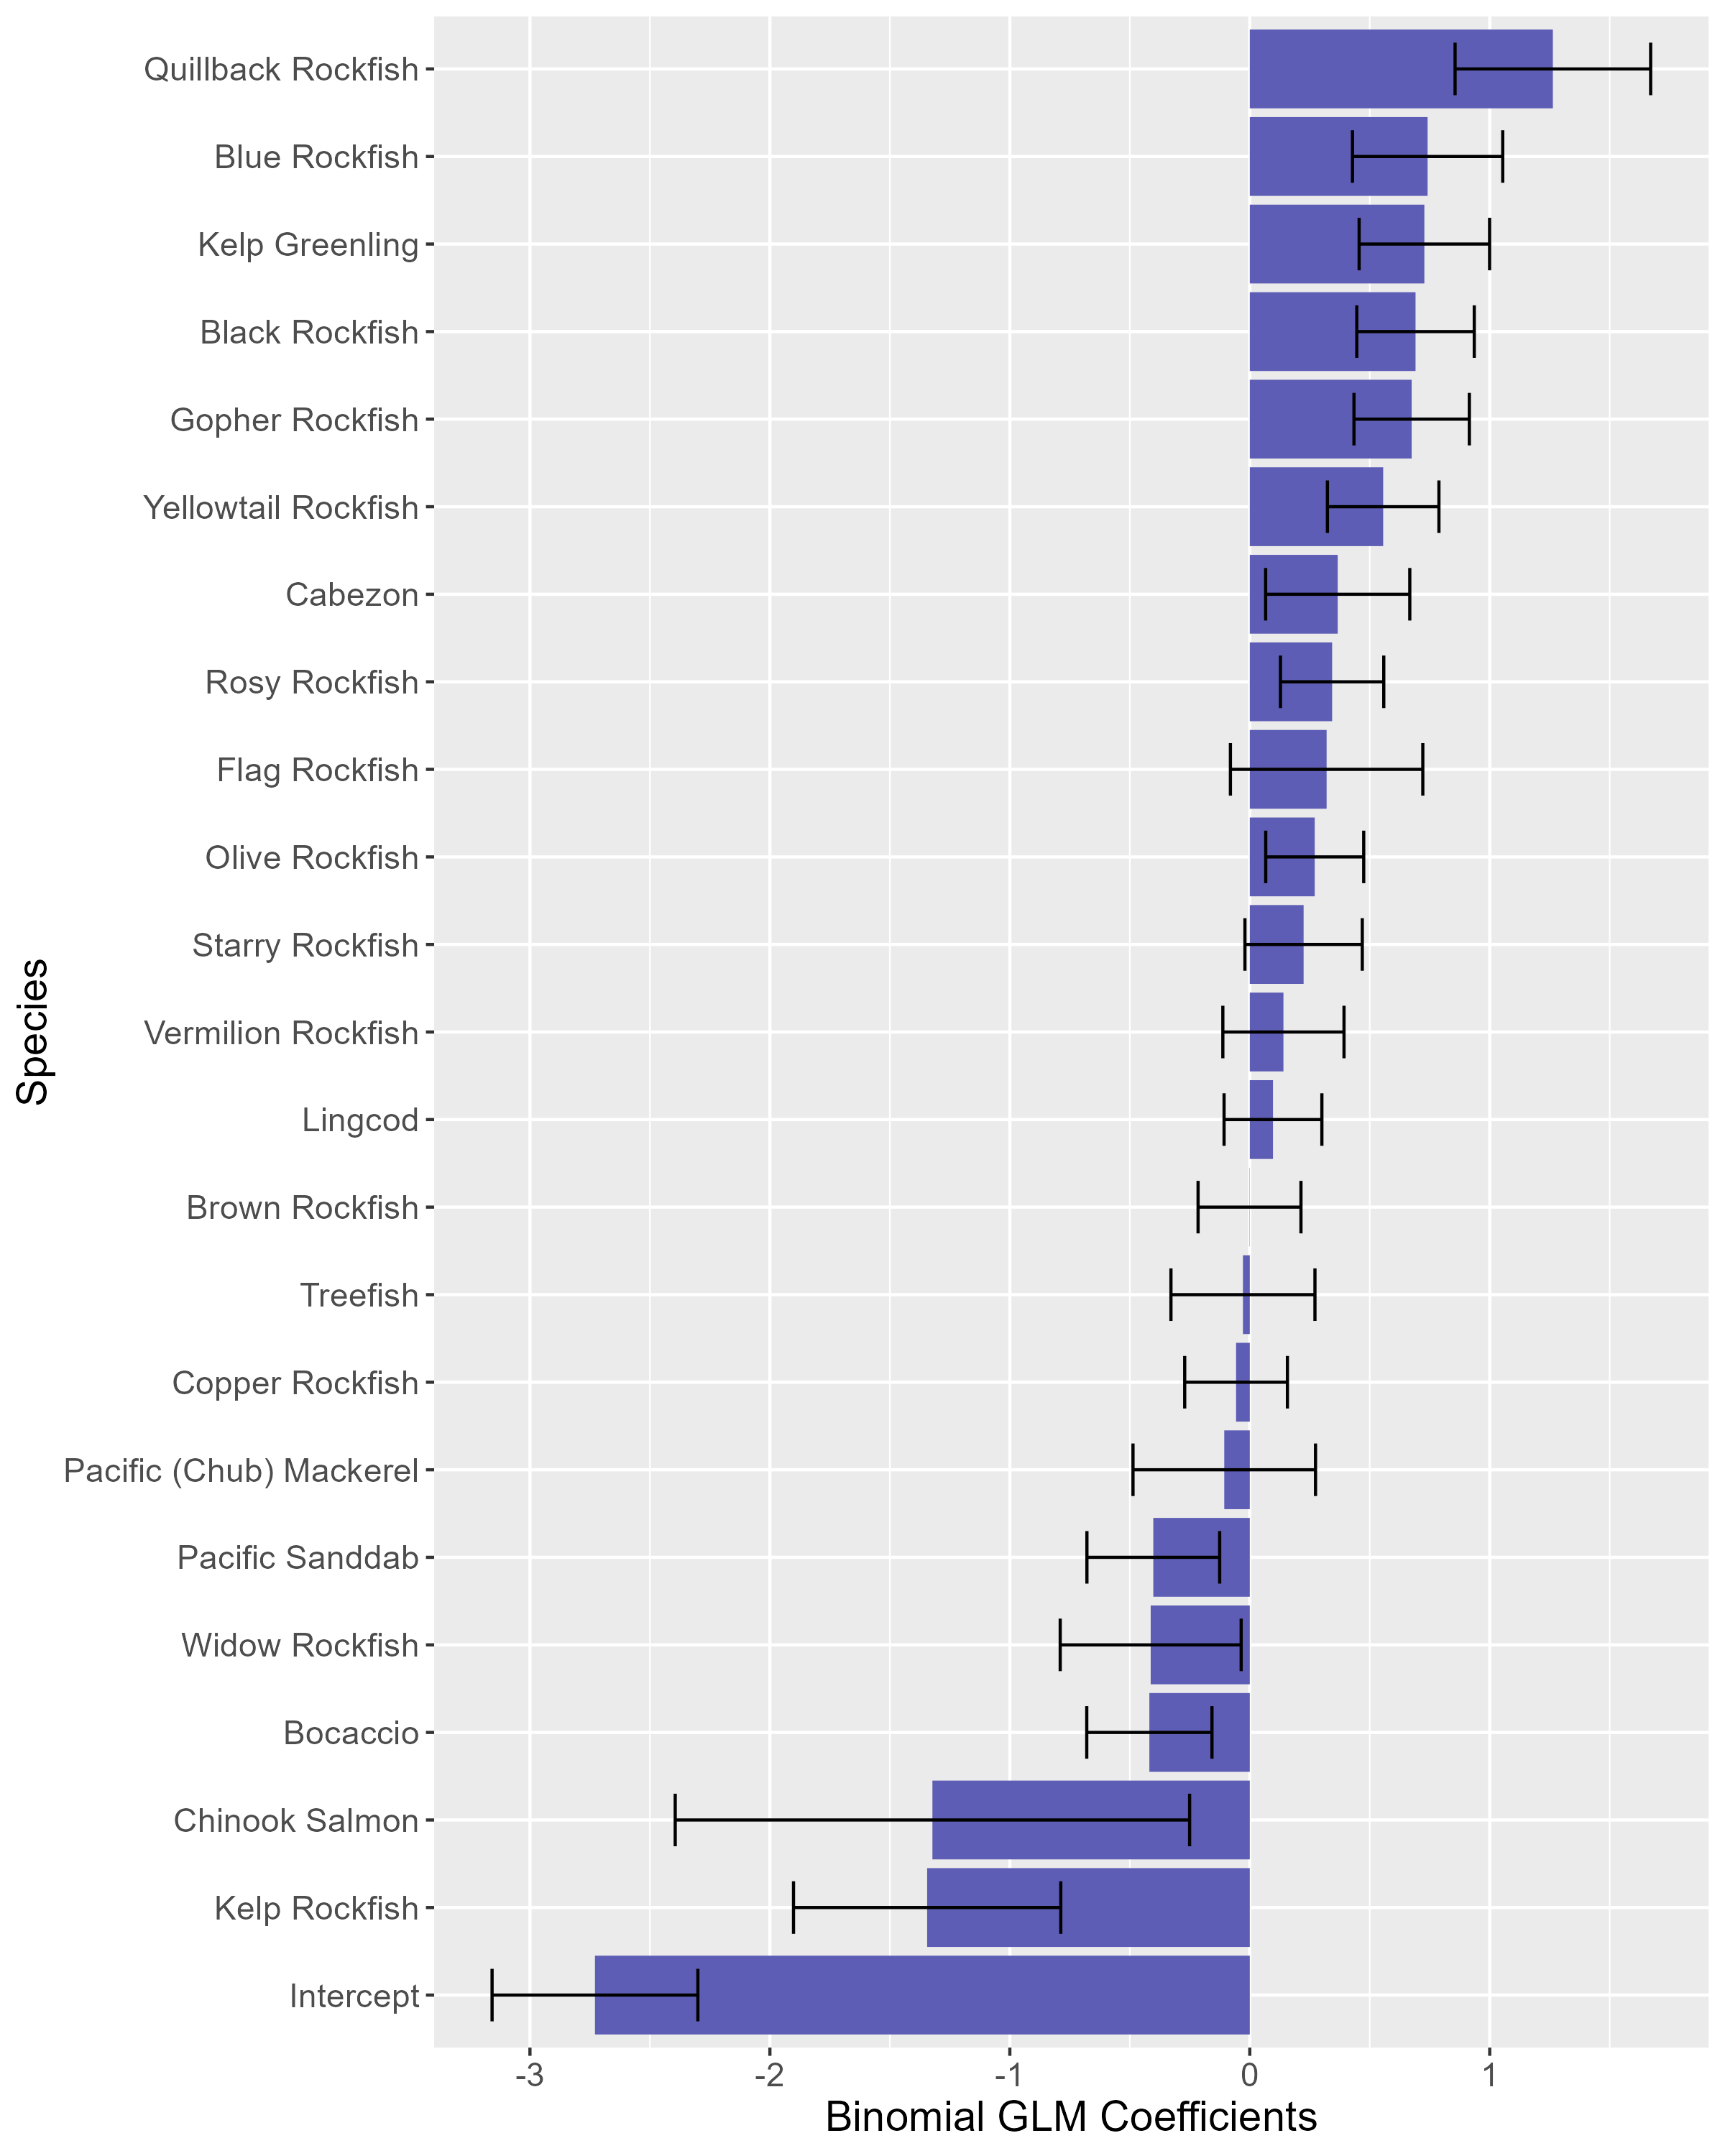
\includegraphics[width=2.75in,height=\textheight]{figures/china_trip_sm.png}

}

\caption{China rockfish trip level}

}

\end{minipage}%
%
\begin{minipage}[t]{0.50\linewidth}

{\centering 

\raisebox{-\height}{

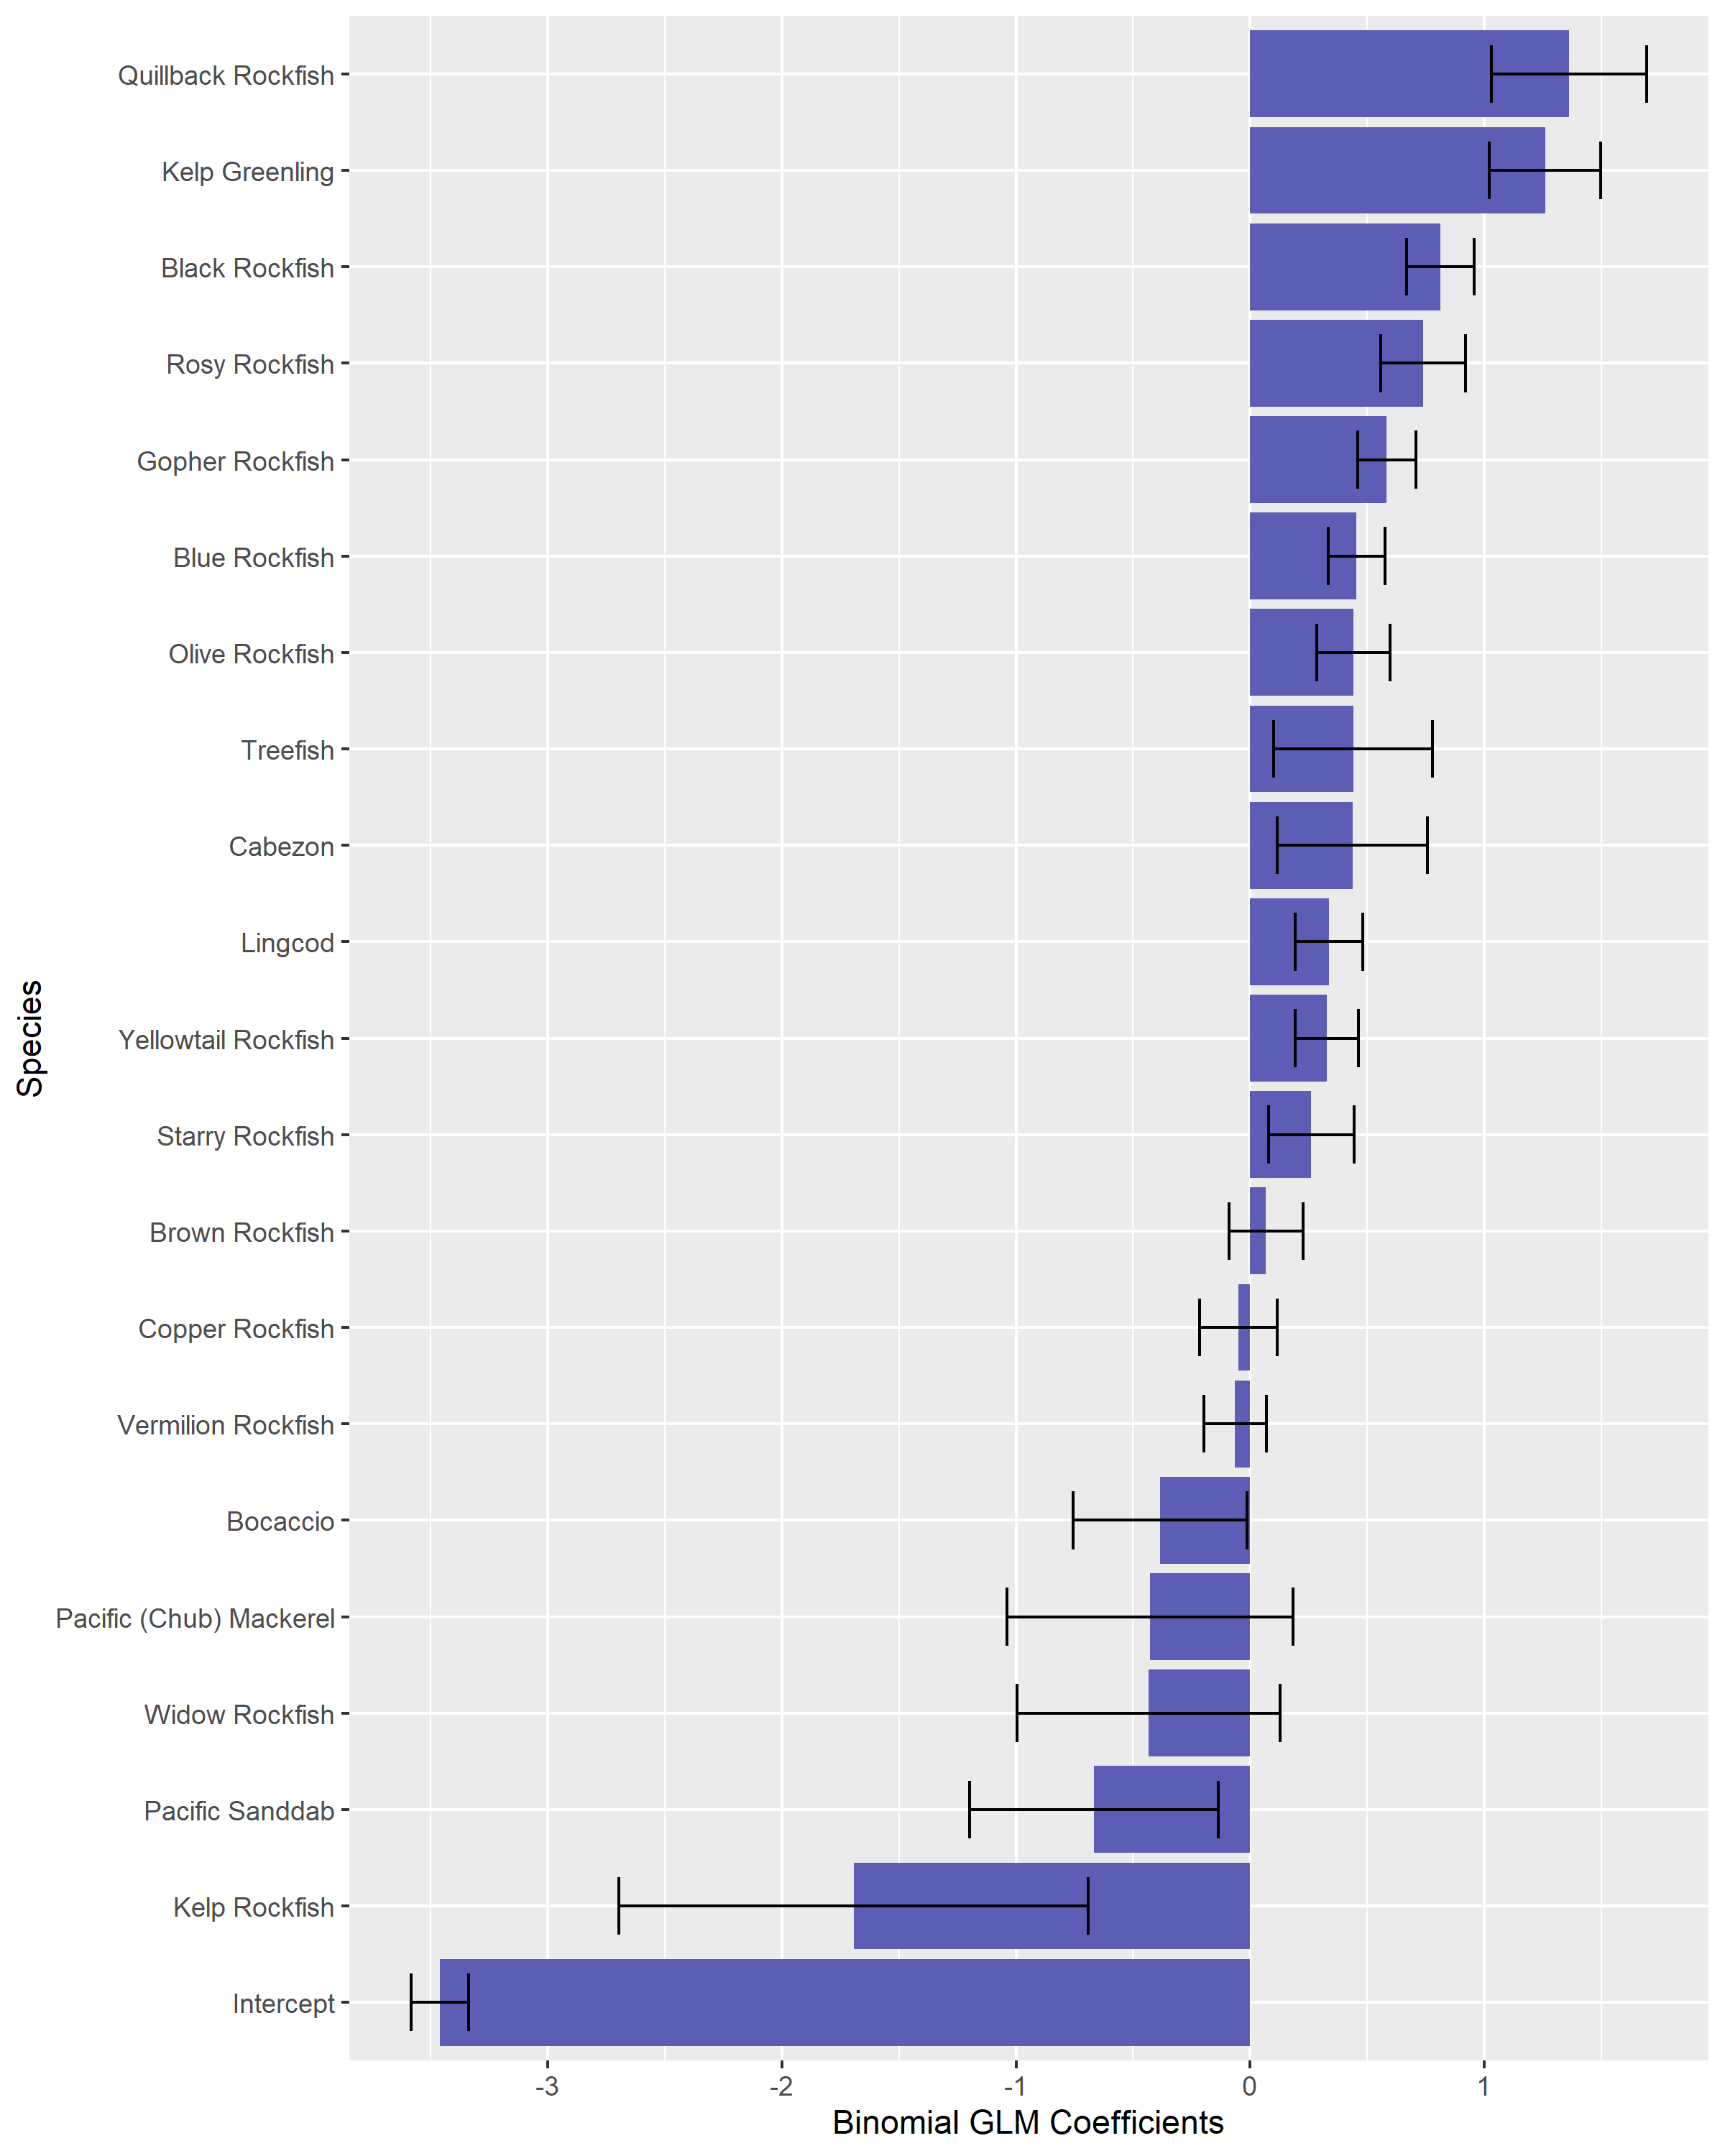
\includegraphics[width=2.75in,height=\textheight]{figures/china_drift_sm.png}

}

\caption{China rockfish drift level}

}

\end{minipage}%
\newline
\begin{minipage}[t]{0.50\linewidth}

{\centering 

The species coefficients from the Stephens-MacCall method at the
trip-level and drift-level for species not presented in the main body of
the paper.

}

\end{minipage}%

\end{figure}


  \bibliography{bibliography.bib}


\end{document}
